\documentclass[12pt]{article}
\usepackage[a4paper, total={15cm,25cm}]{geometry}
\usepackage{titlesec}
\usepackage{graphicx}
\usepackage{float}
\PassOptionsToPackage{hyphens}{url}\usepackage{hyperref}
%\usepackage{fancyhdr}
%\setlength{\headheight}{15pt}
%\pagestyle{empty}
%\fancyhead[L]{110-1 Bio-MEMS Fabrication Homework}
%\fancyhead[R]{鄭泊聲 b07611002}
\usepackage{amsmath}
\usepackage{latexsym}
\usepackage{multirow}
\graphicspath{ {./images/} }
\usepackage[backend=biber, citestyle=numeric, bibstyle=numeric, sorting=none]{biblatex}
\addbibresource{ref.bib}
\usepackage{mathspec}   %加這個就可以設定字體
\usepackage{xeCJK}       %讓中英文字體分開設置
\setCJKmainfont{標楷體} %設定中文為系統上的字型
\newCJKfontfamily[chineseSans]\CJKsans{Noto Sans CJK TC}
\setmainfont{Sabon}
\setsansfont{IBM Plex Sans}
\setmonofont{Roboto Mono}
\XeTeXlinebreaklocale "zh"             %這兩行一定要加,中文才能自動換行
\XeTeXlinebreakskip = 0pt plus 1pt     %這兩行一定要加,中文才能自動換行
\renewcommand{\baselinestretch}{1.35}
\renewcommand{\figurename}{圖}
\renewcommand{\tablename}{表}
\renewcommand{\abstractname}{摘要}
\renewcommand{\contentsname}{目錄}
\renewcommand{\listtablename}{表格目錄}
\renewcommand{\listfigurename}{圖片目錄}
%\renewcommand*{\bibfont}{\footnotesize}
\titleformat*{\section}{\Large \bfseries \CJKsans}
\titleformat*{\subsection}{\large \bfseries \CJKsans}
\titleformat*{\subsubsection}{\bfseries \CJKsans}
\setcounter{tocdepth}{2}

\title{研發新穎線掃描高光譜顯微影像技術}
\author{鄭泊聲\thanks{國立臺灣大學經濟系大學部}
\and 指導教授:張玉明\thanks{國立臺灣大學凝態科學研究中心特聘研究員}}
\date{\today}

\begin{document}
\maketitle
\section*{致謝}
特別感謝張玉明老師將本系統的開發交付給我,並在過程中給予無私的支持與指導。
本系統開發承蒙科技部110學年度大專學生參與專題研究計畫
支持(計畫編號110-2813-C-002-218-M),另感謝實驗室的陳
維良博士帶我了解光學系統的基礎知識、黎文鴻博士協助光路的調整,並承接本研究的後續開發,以及羅詔元博士在LabVIEW程式撰寫給予許多指導,和黃鈺淳在研發過程中鼎力
協助。
\section*{摘要}
\section*{Abstract}
\tableofcontents
\listoffigures
\listoftables
\section{前言與研究目的}
傳統的光譜量測技術,
在光譜儀中,被展開的樣品光譜多半以線性光譜(spectrum)呈現,記錄其在各個波長的訊號強度。對於由單一物質組成的均勻樣品,這樣的觀測方式相當有效率,
但觀測者若想了解樣品在不同位置上的光譜性質差異,則必須對樣品的每個位置分別進行光譜展開,才能建立出一張含有位置訊息的光譜影像(spectral image)
。以最常見的二維掃描來說,必須沿著樣品座標軸上所設定的二維區域進行「面」的掃描,再透過後處理將每個位置的光譜資訊重新建立成一張二維平面的光譜影像。

而線掃描高光譜影像技術,則是將帶有一維空間位置訊息的光譜資訊進行展開,能夠大幅減少光譜影像掃描所需的掃描時間。舉例來說,在一個二維卡式座標中,傳統的雷射掃描共軛焦顯微鏡一次只能對
「一個點」進行光譜展開,
若要建立一張二維的光譜影像,就必須進行二維的「面掃描」;而線掃描高光譜影像技術,則是對樣品上的「一條線」,將線上每個點之光譜一次性展開,因此,
只要沿著與這條「掃描線」的垂直方向進行一維掃描,就能快速地完成一張二維區域的光譜影像,如此可大幅提升顯微光譜影像的量測速率。

本研究即旨在建立一部完整的線掃描顯微高光譜影像系統,以提升新穎材料與樣品微結構的觀測效率。整個系統的建構,包括以電動載台作為掃描裝置進行各式操控,以及二維影像感測器的操作,還有系統光路架構的設計與開發調整。
最核心者則是系統整合與軟體的使用者介面及功能,以完全自行撰寫的電腦程式來操控載台、影像感測器,確保其之間的匹配,並且進行影像的接合及處理,最後並力求整體操作介面的易用性與功能性,

除此之外,我們希望進一步拓展本系統對於不同樣品,包括新穎材料、生物組織、奈米結構等的觀測領域,因此也希望針對「背焦面影像」(Back Focal Plane)的技術進行探討與整合,
以期能建立一部具有多元光與物質反應(Light-matter interaction)觀測能力的影像系統。

\section{原理探討與文獻回顧}
\subsection{線掃描高光譜影像技術的原理}
\begin{figure}[h]
    \centering
    \includegraphics[width=\linewidth]{hsi_from_object_to_cube.jpg}
    \caption{線掃描高光譜影像的原理}
    \label{fromObjecttoCube}
\end{figure}
本系統所採用的線掃描(Line scan or Push-broom)影像原理,可以圖\ref{fromObjecttoCube}來說明。首先,系統中包含一個簡單的光學顯微鏡,能搭配不同倍率的顯微物鏡使用,該光學顯微鏡會將樣品的像成在一部線光譜儀的入射狹縫上(圖中的input slit),
樣品位置不同時,狹縫上的像也會不同。狹縫上的影像即對應到樣品的「掃描線」,而這部線光譜儀會同時對線上的每個位置進行光譜量測(圖中的dispersion示意),共計512條光譜線會在影像感測器上形成一個二維影像,其Y軸就是與狹縫同向的空間座標,
其X軸則是光譜的波長座標(即是圖中的on sensor image)。

透過這樣的影像系統,我們從影像感測器上擷取一張二維影像(on sensor image),就能得到樣品單線上512個不同位置的光譜,接著只要再對樣品進行單方向的移動掃描,就能將各處單線的光譜影像組合成一張完整的高光譜影像(Hyperspectral image)。
在本系統的設定下,將樣品沿著空間的x軸移動,擷取每個x座標上的線掃描影像後,透過軟體接合,即可得到整個樣品平面的光譜資訊。這樣的影像除了記錄樣品在二維空間的空間特徵外,也包含了每個空間位置的光譜特徵,因此實是一張三維的影像(Data cube)。

\subsection{顯微高光譜影像的發展現況}
顯維高光譜影像技術在研究領域的發展,涵蓋相當廣的層面。觀測的範圍從最常見的樣品螢光
、雷曼散射,到相干反斯托克斯拉曼光譜(CARS)都有\cite{roth2015hyperspectral,zhang2013quantitative, pegoraro2014hyperspectral}。
研究應用的領域,也相當廣泛,尤其以生物相關的研究最為豐碩\cite{leavesley2012hyperspectral,studer2012compressive},而奈米材料相關的研究當然也不再話下\cite{roth2015hyperspectral}。

近期的相關研究更在高光譜影像資料處理有不少突破,過去以影像處裡演算法的開發為主
\cite{manolakis2002detection,nascimento2005vertex}
,並以影像偵測的相關研究成果較為豐盛\cite{manolakis2009there},到近年更有將深度學習應用於高光譜影像處裡的成果\cite{chen2014deep}。

目前市面上所販售的高光譜影像系統,則多數以巨觀尺度的觀測為主,尤以生產線上的品管應用,或是廢棄物處理的分類等尤為顯著。\cite{useCaseInline}這類型的應用,多數也是採用與我們類似的線掃描技術,
但也有其他較特別的高光譜量測方式,例如\cite{FTHY}在時域以傅利葉轉換的得到光譜資訊,號稱能建立出連續的光譜,擁有無限的光譜解析度。\cite{globalHY}的全域高光譜(Global hyperspectral imaging)
影像技術則是每次在不同的波長下拍攝樣品的二維影像,換句話說,是沿著光譜軸,而非空間中的x或y軸進行掃描。

\subsection{實域與動量域的成像原理}
動量域成像的理論基礎是傅立葉光學,而傅立葉光學的數學核心即是傅立葉轉換。在光學領域,透過傅立葉轉換,能將實域\textbf{位置}的光線訊息,轉換為動量域\textbf{散射角度}的光線訊息。以數學語言來說,
原本以\(f(x)\)定義的光學訊息,代表的是每個x位置上的光線,透過傅立葉轉換\[E(k_x)=\int_{-\infty}^{\infty}f(x)e^{ik_xx}dx\]後,
將呈現出在每個角動量\(k_x\)方向上的光線資訊。

傅立葉光學最簡單的實例就是干涉現像,在光圈或狹縫背後的干涉圖樣,即傅立葉光學的所呈現出的動量域影像。除此之外,
傅立葉光學的概念也早已廣泛應用,例如全像攝影將光線的二維空間資訊加上角度資訊,建立出會隨著觀看角度而變化的影像。傅立葉光學也被應用於空間濾波器的設計,
透過在動量域對光線進行濾波,再到實域成像,能將影像中不同頻率的雜訊移除。
\begin{figure}[h]
    \centering
    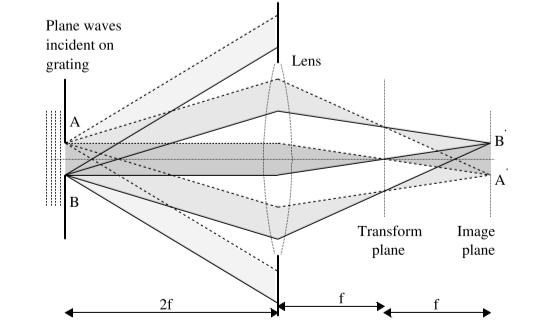
\includegraphics[width=\linewidth]{bfp.png}
    \caption{背焦面成像原理\cite{lightfantastic}}
    \label{bfpimage}
\end{figure}

在本計畫中,我們將以「背焦面影像」來實現動量域的觀測。背焦面影像的技術,可以
透過圖\ref{bfpimage}中的光線示意來理解。在圖\ref{bfpimage}中,
來自樣品上同一\textbf{位置}的光線,將會在實域成像平面(圖\ref{bfpimage}中的Image plane)的同一對應位置匯聚,因此實域影像代表光線的空間位置訊息。
而來自樣品上同樣散射\textbf{角度}的光線,會在背焦面(圖\ref{bfpimage}中的Transform plane, 傅立葉轉換面)的同一個對應位置匯聚成像,因此背焦面影像將代表光線的散射角度。
由此可見,來自樣品實域的光線,若在背焦面成像,就相當於經過了一次傅立葉轉換,由實域轉換至動量域,因此背焦面也被稱為傅立葉轉換面。
在透鏡的成像側,我們能夠選擇於實域的成像面上成像,或是在動量域的背焦面上成像。
在背焦面成像,即能在動量域觀測光線,同時也可以在該平面進行濾波或其他光線的調變,以對實域做影像處理。

若將圖中的透鏡想像為顯微鏡的物鏡與成像鏡,則可以輕易了解,只要分別在成像面與背焦面觀測,
即可在實域影像與動量域影像之間切換。
但由於多數顯微物鏡的背焦面位在鏡筒中,無法直接在該處成像,因此本研究參酌其他文獻\cite{bfpimage}所描述的方式,
透過加上另一片成像鏡,將原本的背焦面影像移動(relay)至易於成像的位置,如此才能在同一部影像感測器上切換實域與動量域的觀測。
在圖\ref{path}中,樣品的發散光經物鏡後,透過L3透鏡匯聚於針孔處。在針孔後放置一個L4透鏡,與針孔的距離正好是L4的焦距,此時針孔處的影像就相當於是L4的待測物,
若將光譜儀或CCD放置於L4的背焦面,即可觀測樣品的動量域影像;若在L4後方加上另一成像鏡L5,則可在L5的焦點觀測到實域影像。
\begin{figure}[h]
    \centering
    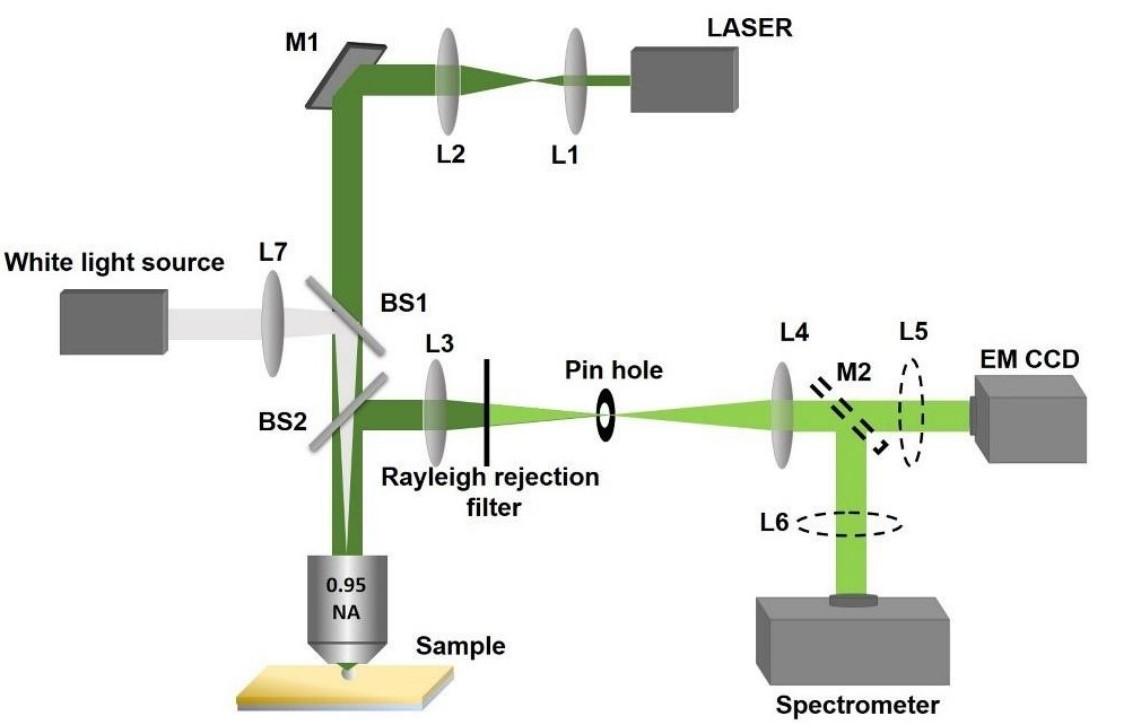
\includegraphics[width=\linewidth]{bfppath.jpg}
    \caption{動量域影像的成像光路參考\cite{bfpimage}}
    \label{path}
\end{figure}

在背焦面影像的領域,則多半以應用於微結構與光線散射分布的研究為主。例如以背焦面影像觀測電漿子的研究,
或是光子晶體相關的研究\cite{hartmann2013radiation,zhang2014back,wagner2012back}。
透過干涉的背焦面影像技術實現其他微結構觀測方法的研究也有許多,例如透過背焦面影像實作光線散射觀測的研究\cite{davidson2006interferometric},
或是橢圓偏振技術的實現\cite{feke1998interferometric}。

近年來專注於高光譜技術與背焦面影像技術整合的研究則較為稀少,在一些高光譜影像系統開發的研究中,
確實有提及在背焦面對影像進行調變\cite{gao2010snapshot},但與本研究希望以背焦面影像成像為主的目標仍有差異。
\section{研究方法}
本研究將整體系統開發分為以下三個階段,以求按部就班,從線掃描高光譜的基礎原理與技術開始,到更複雜的顯微影像光路整合,最後進入更完善的光譜影像瀏覽、
分析功能,與背焦面影像技術的開發。
\subsection{第一階段: 巨觀實域觀測} \label{macroreal}
本階段的目標是了解線掃描高光譜影像技術的基礎原理,採較單純的光路規劃,亦是最常見的高光譜影像技術系統,將用於尺寸在公分等級的樣品之實域觀測,系統將採用外部線光源的方式照明,
以電動載台移動樣品進行掃描,且使用廣角焦距的物鏡搭配線光譜儀,觀測樣品的反射光譜影像。

在這階段,我們希望可以透過本系統更深入了解高光譜影像對光源的要求,
例如: 是否一定必須使用線光源?光源需涵蓋的光譜範圍必須多大?強度必須多強?
各個光學元件的NA匹配、是否需要合適的濾波、如何節省所需的空間與元件數量等,也都是開發本子系統的過程中希望習得的知識與經驗。

另外,在本階段的軟體開發部分,主要重點將是後端軟體中系統硬體操控、掃描影像接合、矩陣運算等基礎項目。
\subsection{第二階段: 微觀實域觀測} \label{microreal}
本階段開發之系統的主要應用場域是微米等級樣品的實域觀測,因此將原本使用的廣角物鏡改為一套顯微鏡系統,並將載台掃描改為galvo掃描,與線掃描高光譜影像系統整合,兩套系統之間的整合問題可能是本階段最大的挑戰。

傳統顯微物鏡的NA、景深、各波段穿透率、成像圈\ldots 等規格,是否能和符合高光譜影像之需求,是本子系統開發的重點項目。
如何操控雷射、同步galvo掃描、如何確保樣品上每個位置的光線皆能同步精確量測、如何實作線掃描等,都是本系統所必須完成的目標。

在軟體部分,本階段最重要的目標是前端介面的開發,由於整個系統的使用者操作都將以軟體介面達成,將操作介面設計的直觀易用,並提供各種光譜量測所需的功能,非常重要。本階段所開發的軟體及硬體,將延用至第三階段繼續精進,

\subsection{第三階段: 動量域觀測} \label{momentum}
本階段我們將在第二套子系統的光路中加入可進行動量域影像的量測功能,因應這樣的研究需求,我們相信在光路的設計規劃上勢必更加複雜。
如何設計出能在實域觀測與動量域觀測之間切換的光路,是本系統的主要目標與挑戰。有效地建立能夠在背焦面實作雷射共軛焦顯微高光譜影像的系統後,
本計畫規劃的光學系統即告完備。
\footnote{惟動量域的光譜分析屬高等研究領域,本計畫的研究目標僅設定在於光學系統與量測技術的建立,研究樣品的背焦面光譜影像分析將不在本計畫的研究範疇。}

同時,本階段的軟體開發,除了演算能力、操作介面的持續精進外,高光譜影像的瀏覽、分析功能,對於包括背焦面影像在內的各種光譜觀測方式極其重要,將是本階段軟體開發的重點。

\subsection{軟體開發} \label{software}
本研究的軟體系統,主要功能在於線掃描高光譜影像擷取與分析功能的建立,相較於傳統雷射掃描方式,高光譜影像一次須處裡的資料更龐大,軟體系統必須有效地進行資料擷取與分析。另外,如何計算不同物鏡下分光儀不同的空間解析度,
並在CCD上的合適範圍讀取資料進行影像拼接,也是軟體系統開發的關鍵問題。
除此之外,掃描元件的控制、影像的截取與呈現、CCD的同步控制、使用者介面的建立等,亦是軟體開發的範疇。影像資料分析功能的建立,更是軟體開發後期的主要任務,尤其面對不同觀測域的影像,分析功能的內容勢必更加複雜。
我們將採用LabVIEW來開發操作介面(GUI)及應用程式主體,並以C++實作動態含式庫(.dll)輔助後台的影像處理及資料流。

\section{研究結果與討論}
\subsection{第一階段: 技術驗證}
\subsubsection{巨觀用系統硬體}
\begin{figure}
    \centering
    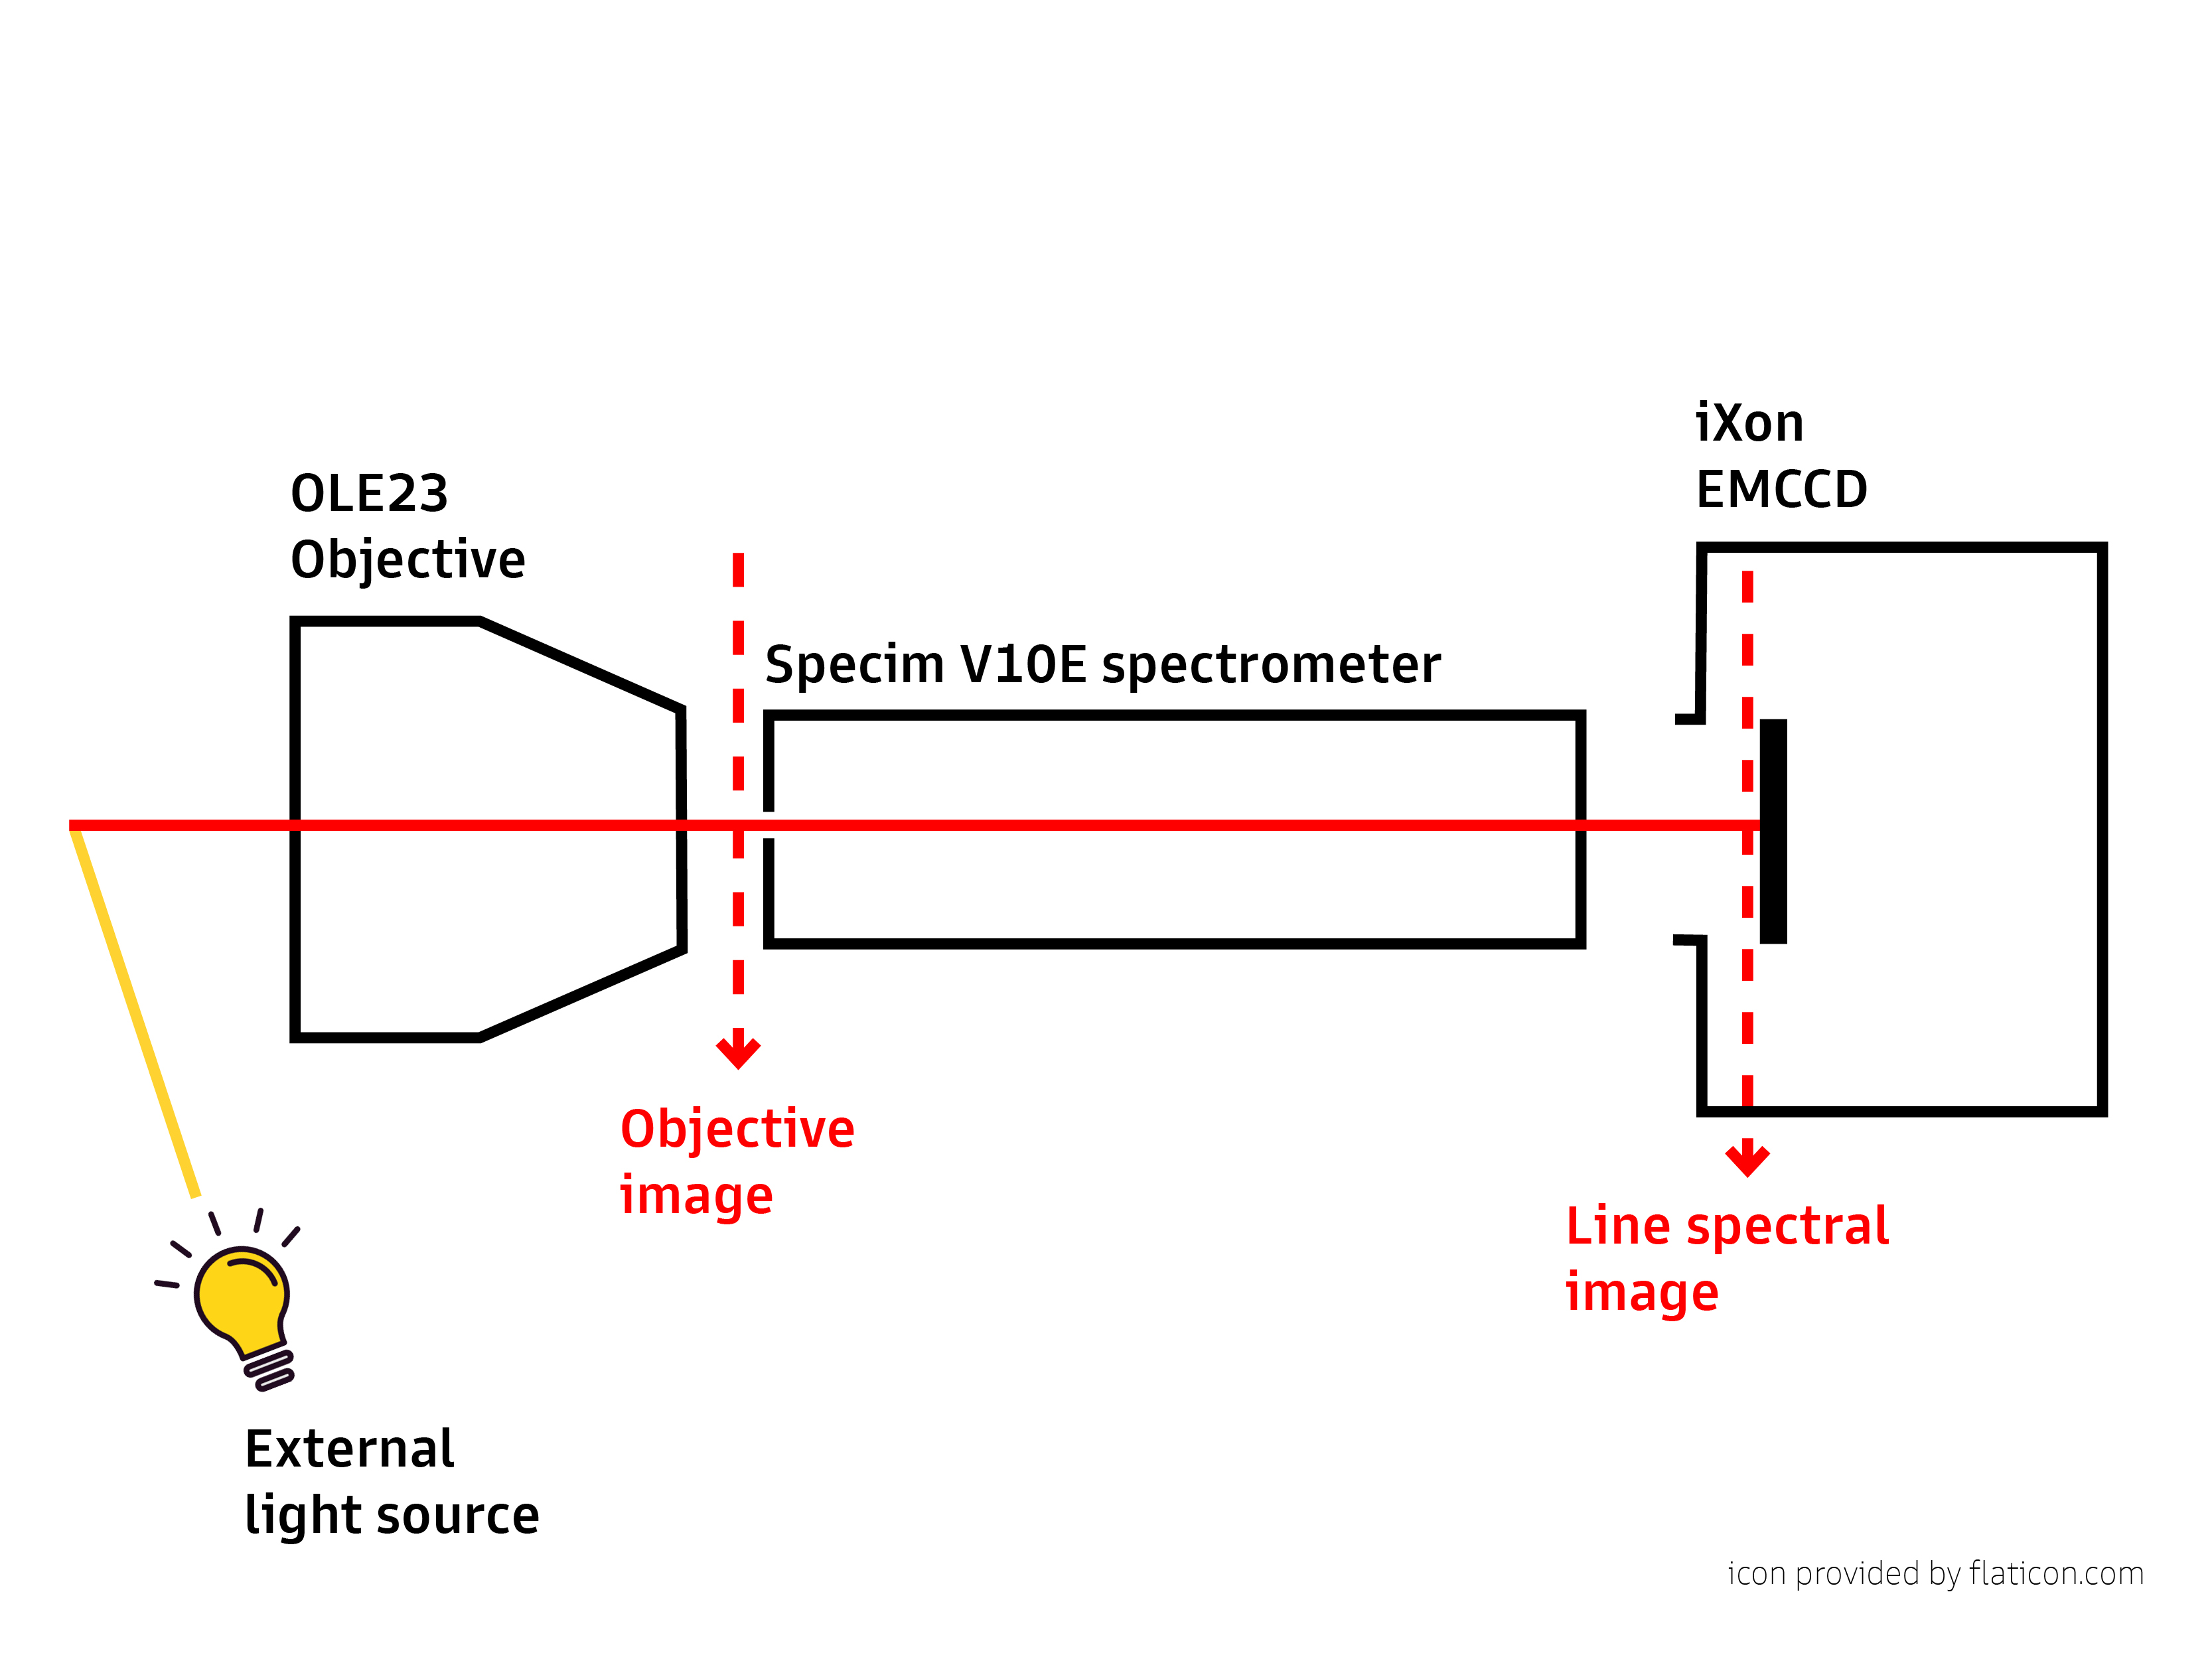
\includegraphics[width = 0.9\linewidth]{lightPath.jpg}
    \caption{巨觀系統光路圖}
\end{figure}
第一階段系統是為了在巨觀尺度下觀測實域影像而設計,在本計畫中也是作為概念驗證與軟體開發的雛型。
在這個階段中,整個系統主要由以下幾個部建構成:
\begin{enumerate}
    \item Specim V10E 線光譜儀
          \begin{itemize}
              \item 搭配 Specim OLE 23(mm) 物鏡
              \item 光譜範圍: 400-1000 $nm$
              \item 入射狹縫寬: 30 $\mu m$
              \item 成像尺寸: Image size: $6.15(spectral) \times 14.2 mm$
          \end{itemize}
    \item Andor iXon DU897 EMCCD
          \begin{itemize}
              \item 512 $\times$ 512 pixels
              \item 8.2 $\times$ 8.2 mm
              \item TE cooler
              \item Electron Multiplying gain
          \end{itemize}
    \item Suruga Seiki 電動載台
          \begin{itemize}
              \item 搭配 D120 控制器
          \end{itemize}
\end{enumerate}
由於V10E線光譜儀的成像尺寸與iXon的正方形CCD尺寸並不同,因此當兩部儀器接合使用後,有部分的像是我們無法觀測到的,如圖\ref{figure: image size}所示,
我們將能在系統中能到看到V10E的整個光譜範圍,但觀測物的Y軸方向,卻因為iXon CCD的高度較小,因此無法完整觀測。

\begin{figure}[t]
    \centering
    \includegraphics[width=0.5\linewidth]{imagesize.jpg}
    \caption{Image size when combined}
    \label{figure: image size}
\end{figure}

\begin{figure}[t]
    \centering
    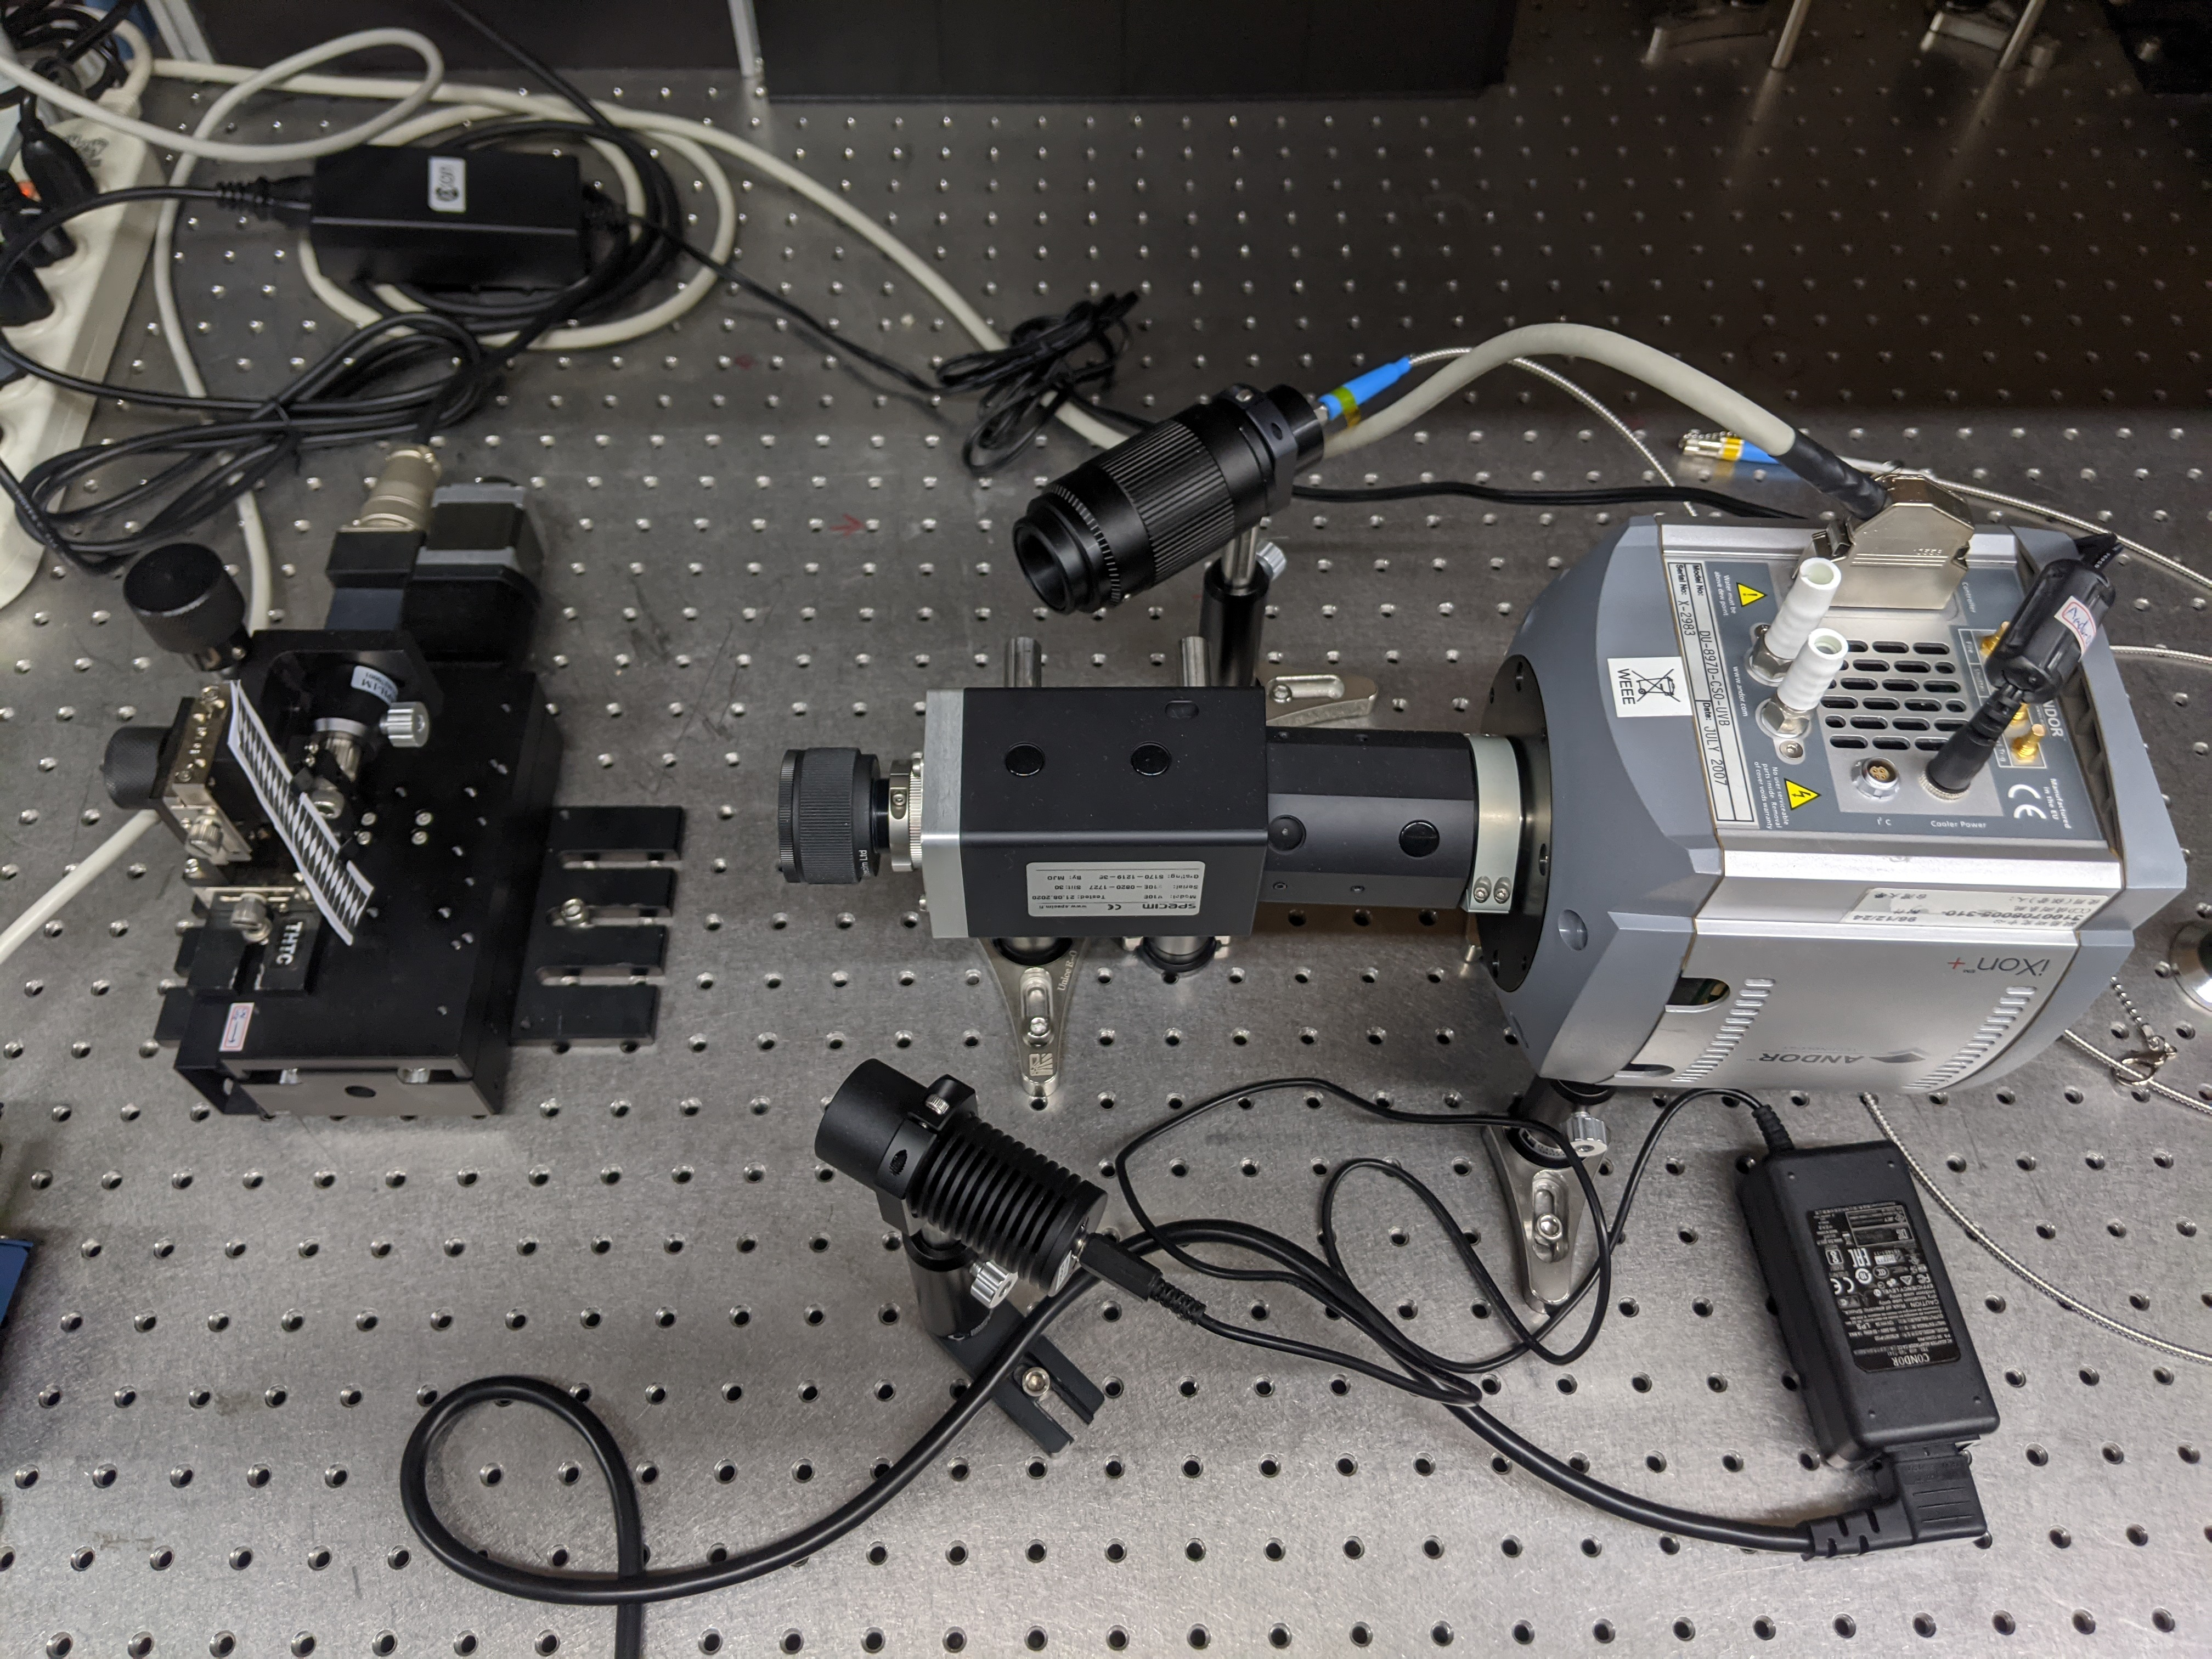
\includegraphics[width=0.65\linewidth]{PXL_20210723_094307842.jpg}
    \caption{Stage, spectrograph, ccd}
    \label{figure: 1 stage setup}
\end{figure}

圖\ref{figure: 1 stage setup}呈現出第一階段系統的樣貌,在照片中另外可以看到LED光源,從外部的黑色手電筒照射觀測物。
\subsubsection{Order Blocking Filter}
由於Specim V10E的前玉為一狹縫,光線進入後,理應會發生單狹縫干涉,產生二階影像(Second order image),因此Specim系統中尚須搭配一個
二階濾鏡(Order Blocking Filer),根據原廠的說明書,該濾鏡可以C-Mount安裝,或是直接黏貼在影像感測器上,不論以何種方式安裝,
皆須盡量靠近影像感測器,實務上與影像感測器不宜超過6mm的距離\cite{manual}。
\begin{figure}[t]
    \centering
    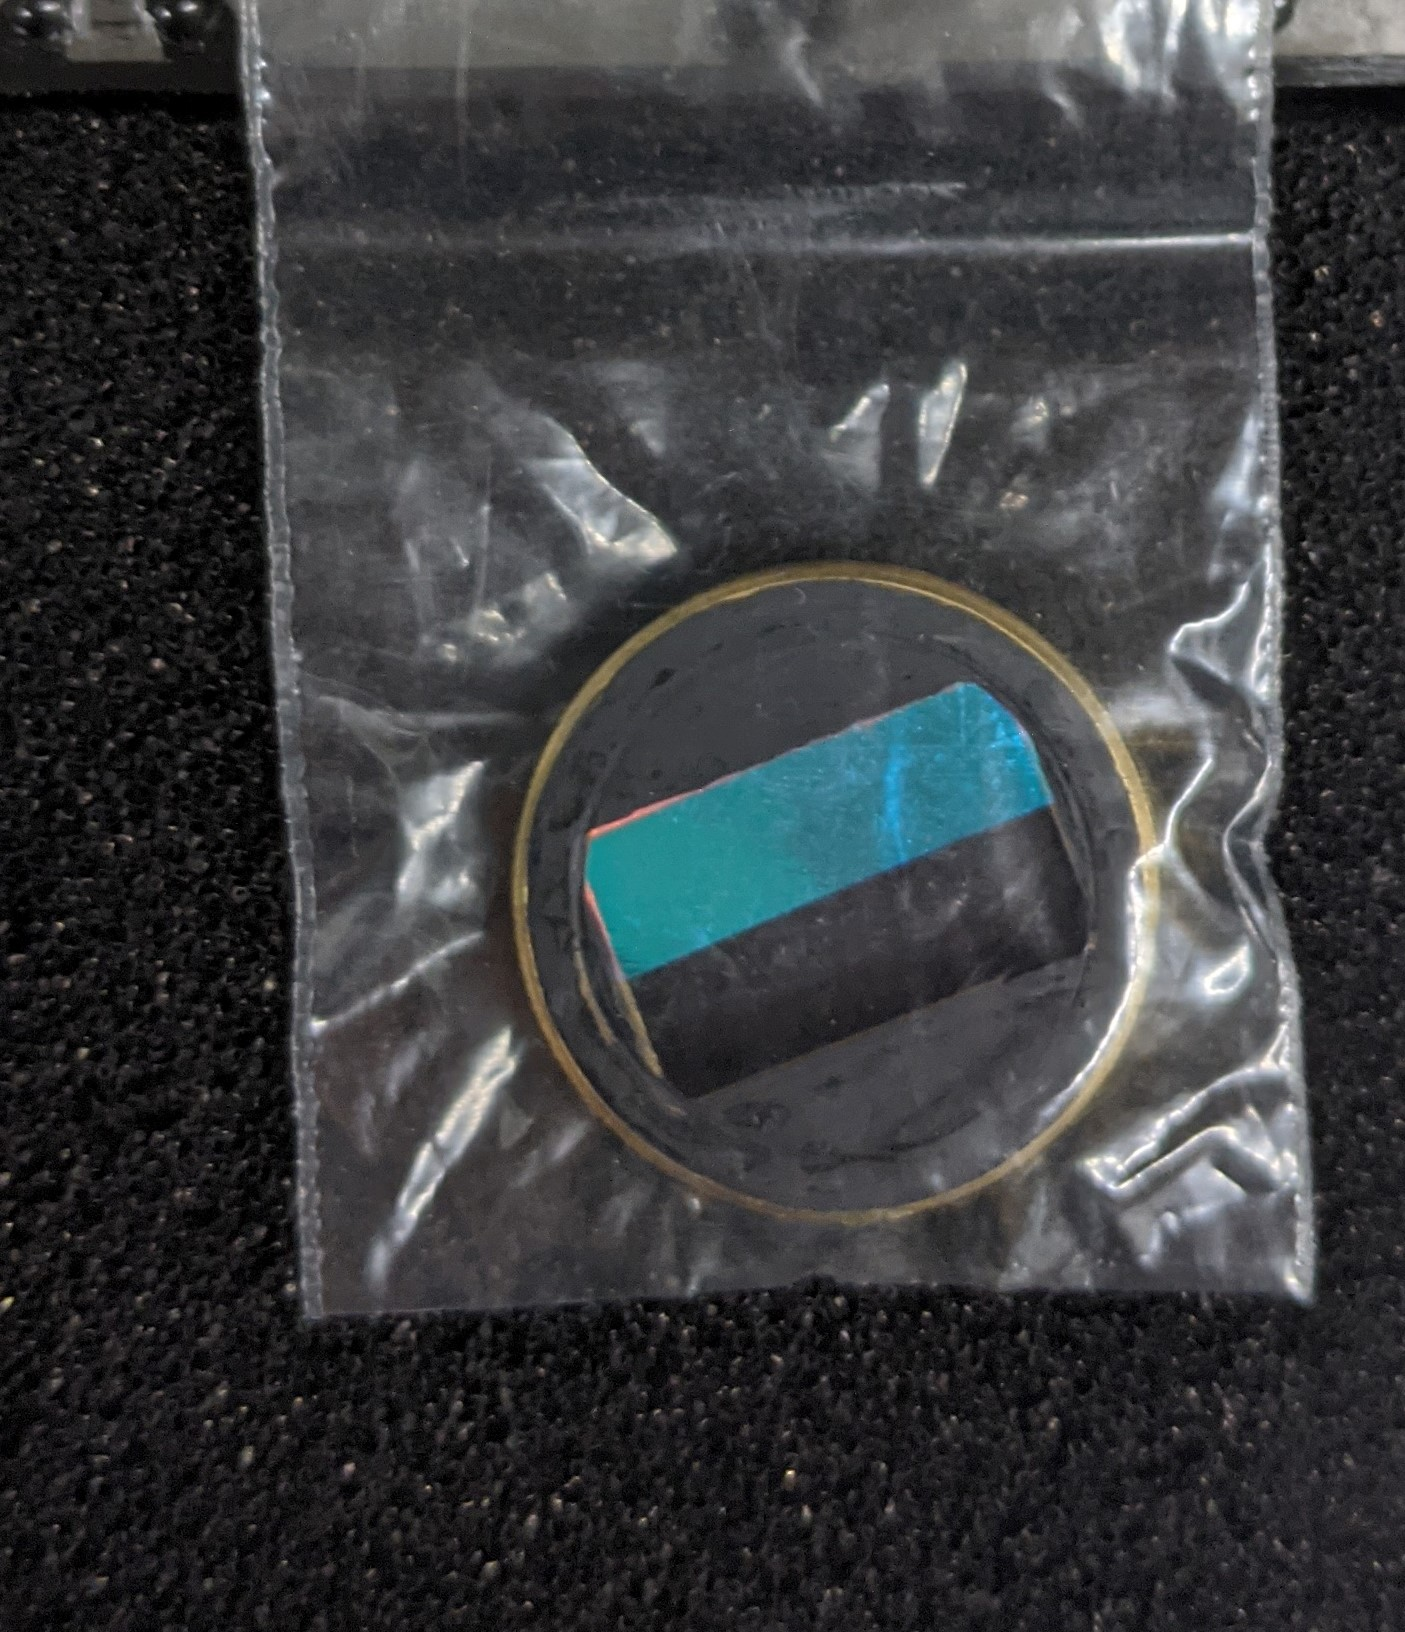
\includegraphics[width=0.5\linewidth]{PXL_20210723_094341395.jpg}
    \caption{The order blocking filter.}
    \label{figure: obf}
\end{figure}
觀察該濾鏡的外觀,可發現其阻擋二階干涉影像的方式,應該就是在鏡面上二階影像出現的位置鍍上塗層進行濾波。由於我們的系統內,不宜將濾鏡直接黏貼在昂貴的iXon EMCCD上,
原本希望以C-mount方式安裝,但可行的安裝位置與影像感測器的距離都會超過6mm,就算客制專用的c-mount轉接環,仍至少會有約9.55mm左右的距離,我們擔心這樣反而會造成該濾鏡阻擋到原初的一階影像,
因此最後決定先不安裝該濾鏡,待過後再來檢視二階影像的影響。事實上,在本系統的往後開發過程中,皆沒有在任何影像中看到二階干涉的影響,
不過這或許一方面是由於我們未曾使用超過30ms的曝光時間,在更長的曝光時間下,二階干涉是否會造成影響,值得後人加以深究。

\subsection{後端軟體基礎}
\subsubsection{三維影像的建立}
本系統所採用的線掃描 (Line scan or Push-broom) 影像原理,就如圖\ref{fromObjecttoCube}所示,系統在拍攝時,實際上從iXon EMCCD上擷取的On sensor image,如圖\ref{figure: linespectrum}所示,其縱軸與分光儀的狹縫同方向,因此也是代表樣品的空間縱軸,
至於影像的橫軸刻度,則是代表不同波長。換句話說,在這張影像的每一個y位置,都有一條光譜線,在iXon EMCCD 512$\times$512像素的設定下,代表每一張on senson image
上都有512個不同位置的光譜線。

為了方便讀者了解三維影像的建立與接合,我們將圖\ref{fromObjecttoCube}重新繪製在圖\ref{fig: form data cube},並加上第二個位置的線掃描影像(on sensor image)的成像過程,以及最終的三維影像data cube接合。
所謂線掃描影像,就是單條掃描線上所拍攝得到的二維光譜影像,也就是線光譜儀在每個掃描位置時成在iXon上的像。

\begin{figure}
    \centering
    \includegraphics[width=\linewidth]{hsi_from_object_to_cube_twin.jpg}
    \caption{三維影像的接合}
    \label{fig: form data cube}
\end{figure}

% 圖\ref{figure: linespectrum}是10x物鏡下,拍攝小型網格圖樣的影像,因此可以看見途中的亮帶與暗帶交錯。

% \begin{figure}[t]
%     \centering
%     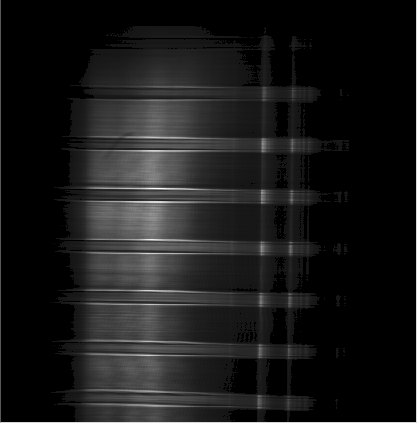
\includegraphics[width=0.5\linewidth]{lineSpectrum1213LDLS.png}
%     \caption{網格的線掃描影像}
%     \label{figure: linespectrum}
% \end{figure}

實際上進行掃描時,只要在樣品上不同位置的掃描線擷取影像,就能得知樣品上每個位置的光譜資訊。在本系統中,樣品放置於在一個電動載台上,我們透過電動載台來移動樣品,以在樣品的不同位置拍攝,
每張線掃描影像皆是512$\times$512像素的二維影像。電動載台每次移動的距離,與總共要移動的距離(也就是掃描的範圍),都是由使用者設定的。
在掃描後,會得到數張這樣的二維影像,疊合後成為一張三維的影像,在程式中,是以三維的矩陣形式處裡。一開始所疊合而成的三維影像,其x,y,z軸分別為波長、樣品y、樣品x軸,
與實際的樣品空間座標有出入,因此必須將矩陣的x與z軸調換(transpose),才能產生出一個與樣品空間相同的影像。該影像即是由512張(由於on sensor image在波長方向有512個pixel)各個波長下的樣品二維影像所組成。

\subsubsection{影像儲存}\label{section: saveTiff}
掃描完成後的三維矩陣,我們將其儲存為TIFF影像格式。TIFF全名維Tagged Image File Format,顧名思義,其檔案中能儲存影像與描述影像的各式標籤(Tag)。
除此之外,Tiff格式支援儲存多個的影像在一個檔案中,故我們能將三維矩陣的每一層二維影像,都儲存在同一個檔案中。使用TIFF格式的另一個好處是,訪間多數的影像瀏覽軟體接支援該格式,
更有許多同樣能夠讀取多層TIFF影像檔案的軟體,如廣泛被使用的ImageJ。

Tiff檔案大致可分為兩部分,前半部分儲存的是檔案中每一張影像的標籤,描述了各式的影像資料,包括公版的影像資料標籤,如影像的像素數與位元等,也包括了我們自行加入的其他影像資料標籤,
如每一層二維影像所在的波長,即是以一個一維陣列的方式儲存為一個自定義的影像資料標籤。

檔案的後半部分,才是各張影像的實際資料。在我們的系統中,每個檔案一律都會包含512張不同波長下的影像,這些影像也各都會有自己的一組影像資料標籤,這512組影像資料標籤也是都儲存在前半部分。

我們使用實驗室過去留下的公版tiff labview library來進行影像檔案的儲存與其中影像資料標籤的管理,在開發初期遇到該library內資料寫入檔案時,端序(byte order)不一致的問題,有些資料是以大端序(big endian),
寫入,有些是以小端序(little endian)寫入,為了配合實驗室Analyser軟體,我們最後一慮皆使用小段序寫入資料。另外,將data cobe寫入檔案時,若將三維矩陣直接寫入,會有array index倒置的問題,正確的寫入方式應該是以for迴圈依序將data cube內的單張影像一張一張寫入。

\subsubsection{座標校正}
當我們成功地建立起三維的影像data cube後,面臨的必要問題即是,要如何確認資料中三個座標軸的尺度?假設我們同樣將data cube的x,y兩軸分別指定為樣品的空間x軸、空間y軸,而z軸則指定為波長方向,
並以一個三圍矩陣(array)的方式來描述與儲存data cube,那麼,座標校正的目的,就是要指定出這個三維矩陣x,y軸上每一個的array index,實際代表的位置,與z軸上每一個array index實際代表的波長。

在此,我們假設線掃描系統的掃描線是空間中的y軸,則這代表掃描時電動載台上的樣品會沿著x軸移動,換句話說,x軸的座標是不需要另外校正的,其座標值以已知的電動載台移動距離即可得知。
至於y軸的座標校正部分,我們只要觀測已知尺寸的樣品,就能得知線光譜儀的視野。在本階段,我們自行設計了一個校正與對焦用的圖樣作為樣品,圖\ref{fig: form data cube}中的樣品就是這個圖樣。

較複雜者是z軸的校正,我們將一個已知光譜的光源,照滿線光譜儀的入射狹縫,並在線掃描影像(on sensor image)上擷取其水平的line profile (接合前的單張線掃描影像,其水平軸實為光譜波長座標軸),
即可繪製出光源的觀測光譜,將這個觀測光譜與光源的已知光譜進行比較,找出其光譜上相似的特徵,紀錄觀測光譜上這些特徵的所在像素,並以這些像素點與已知的光譜特徵所在波長,以線性回歸方式計算其減量線,
即可計算出z軸上每個像素所代表的實際波長。

\begin{figure}[t]
    \centering
    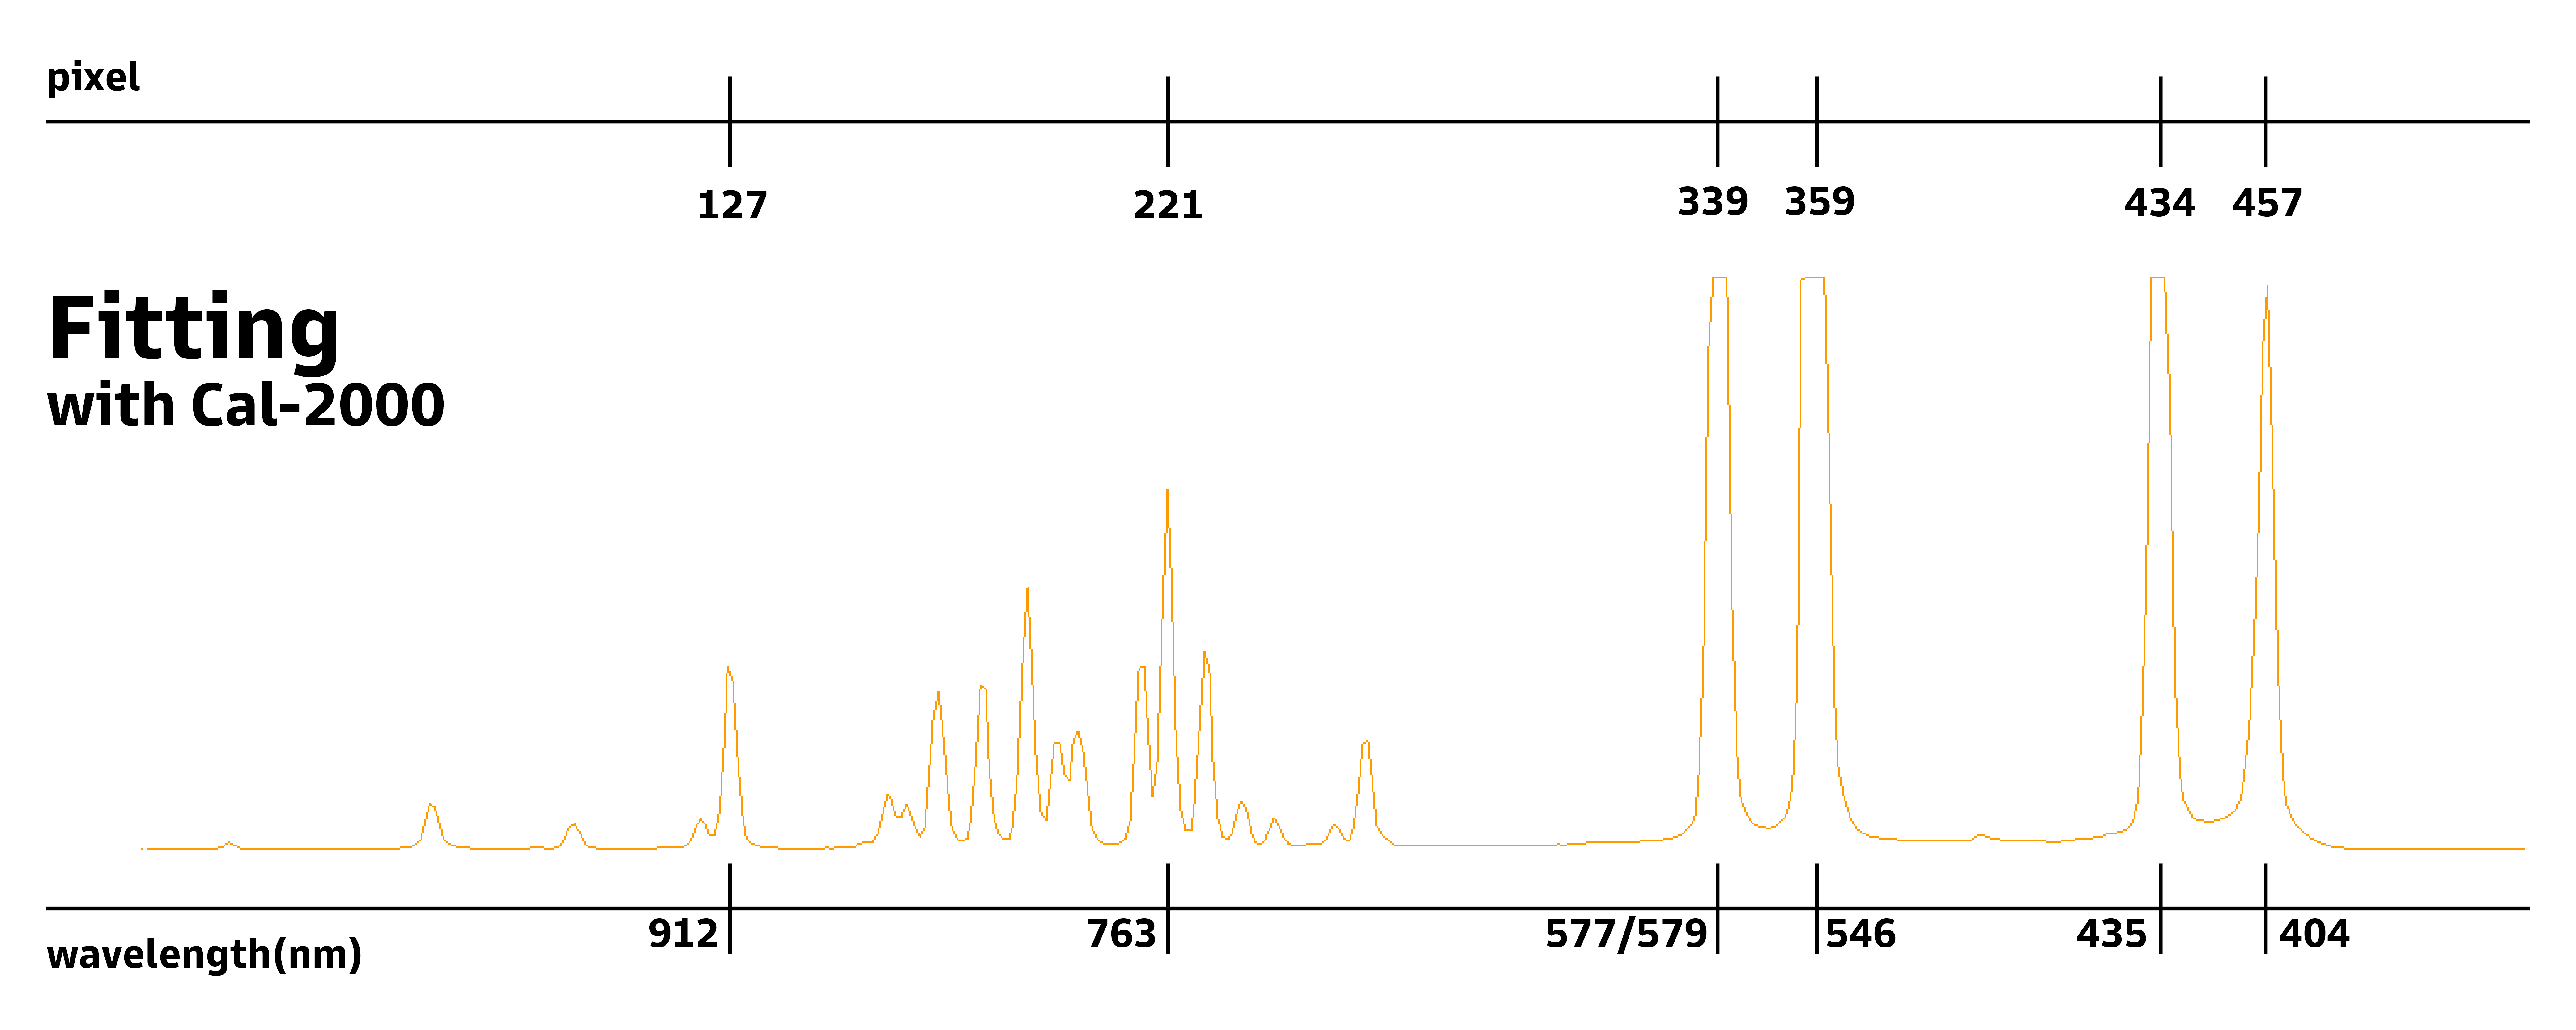
\includegraphics[width=\linewidth]{fitting.jpg}
    \caption{以cal-2000進行校正}
    \label{figure: fitting}
\end{figure}
\begin{figure}[t]
    \centering
    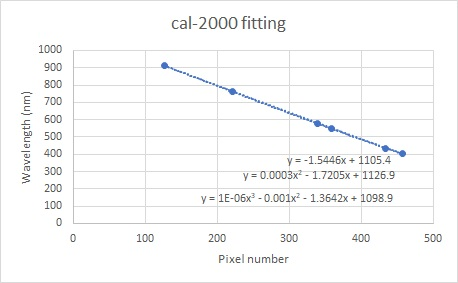
\includegraphics[width=\linewidth]{cal-2000fitting.jpg}
    \caption[]{波長軸校正減量線\protect\footnotemark}
    \label{figure: fit curve}
\end{figure}

\subsection{第二階段: 系統開發}
\begin{figure}
    \centering
    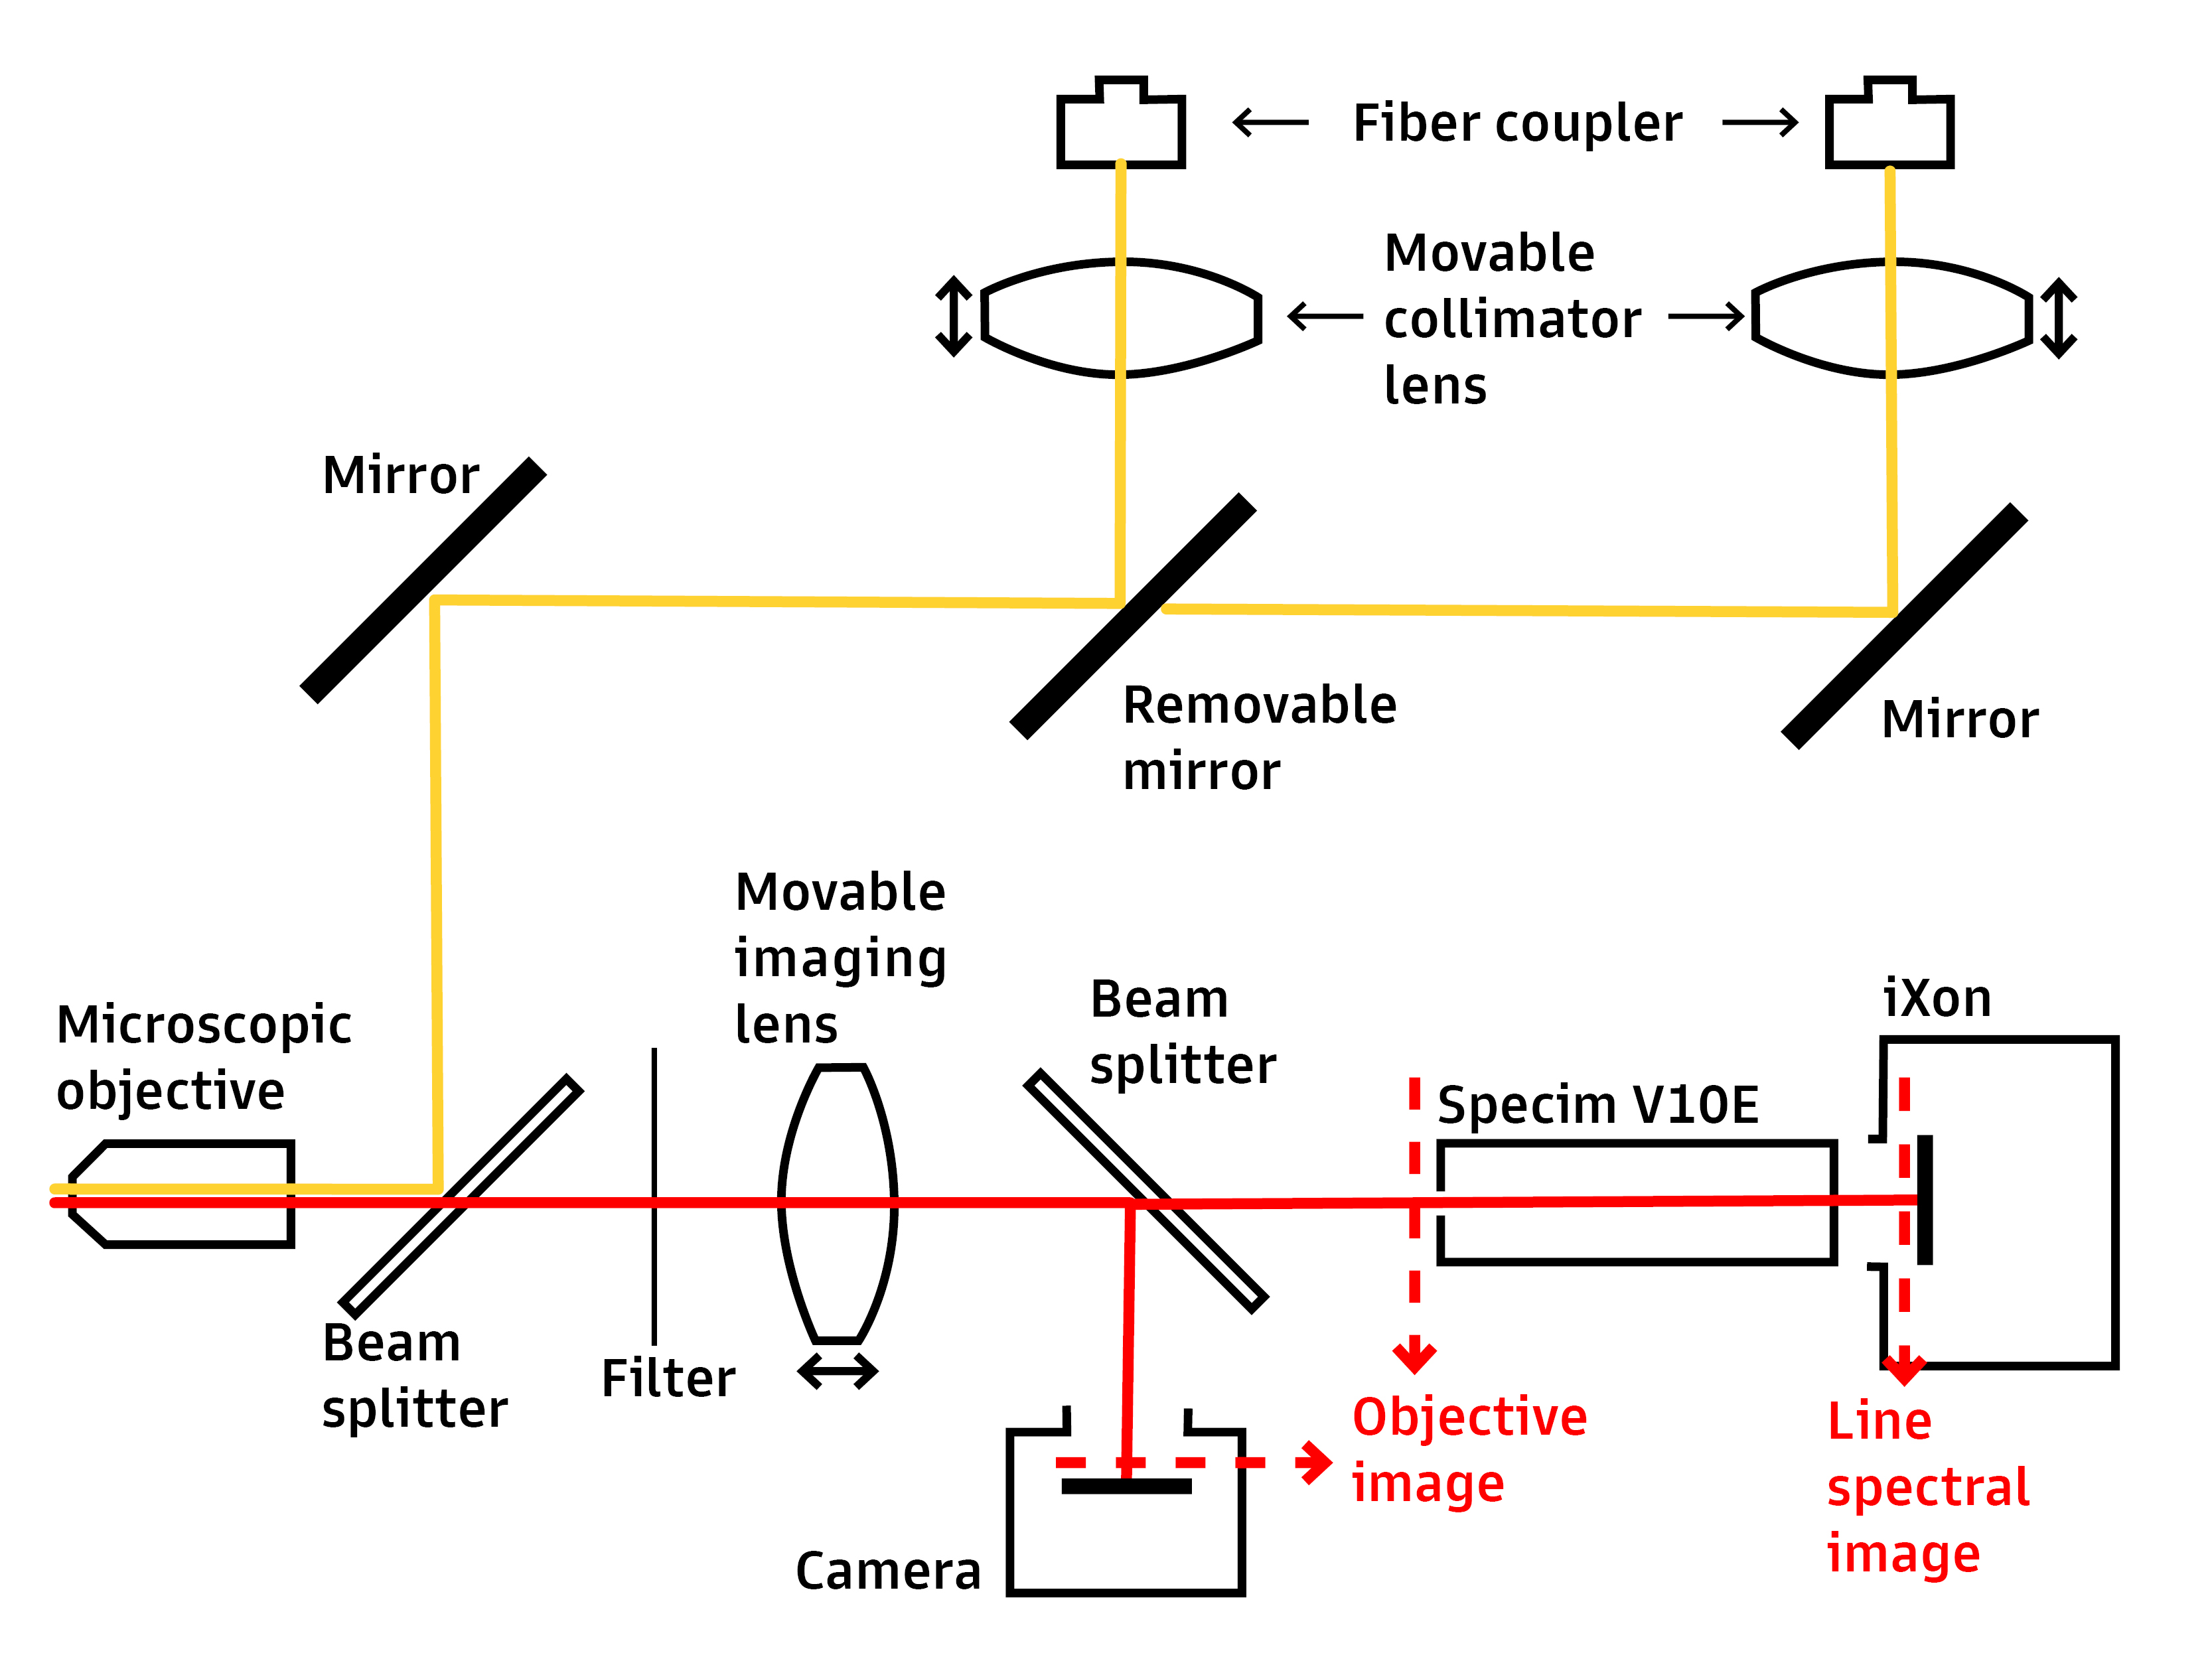
\includegraphics[width = 0.9\linewidth]{lightPath2.jpg}
    \caption{微觀系統光路圖}
    \label{fig: micro path}
\end{figure}
第二階段的系統,主要目的在於將同樣的線掃描技術,應用於微觀尺度,硬體上的變更,首要就是將原本第一階段所採用的OLE 23mm camera lens,置換成一具簡單的光學顯微鏡。我們採用了Olympus 的10x顯微物鏡,
並搭配15 cm的tube lens (imaging lens),將放大過後的樣品影像成在分光儀的入射狹縫上,至於縣線光譜儀與iXon影像感測器的設置,則沒有不同。

除此之外,系統的照明方式也有改變。原初以外部照光的方式,對於所需照明範圍相對較小的顯微影像來說,會浪費較多光源,也不適合進行顯微雷射螢光等觀測,
因此將照明方式改為內部照明,系統上有兩個光纖collimator,能夠彼此切換。光源經過tube lens (imaging lens)匯聚在物鏡的背焦面上,通過物鏡後變成平行光,以期照射在樣品上的光線最為均勻。

裝設物鏡的鏡架,能夠上下移動以進行對焦,光源的tube lens也能微調位置。物鏡的tube lens雖然裝設在可調的鏡筒內,但不應任意移動。至於電動載臺的裝設與使用,則沒有不同。
系統上另外再成像進入分光儀狹縫前,已一片半反射鏡將OM影像投至一臺Canon M200相機中,借助其APS-C尺寸的感光元件,能夠完整顯示出OM的視野,以幫助使用者尋找ROI。
\begin{figure}
    \centering
    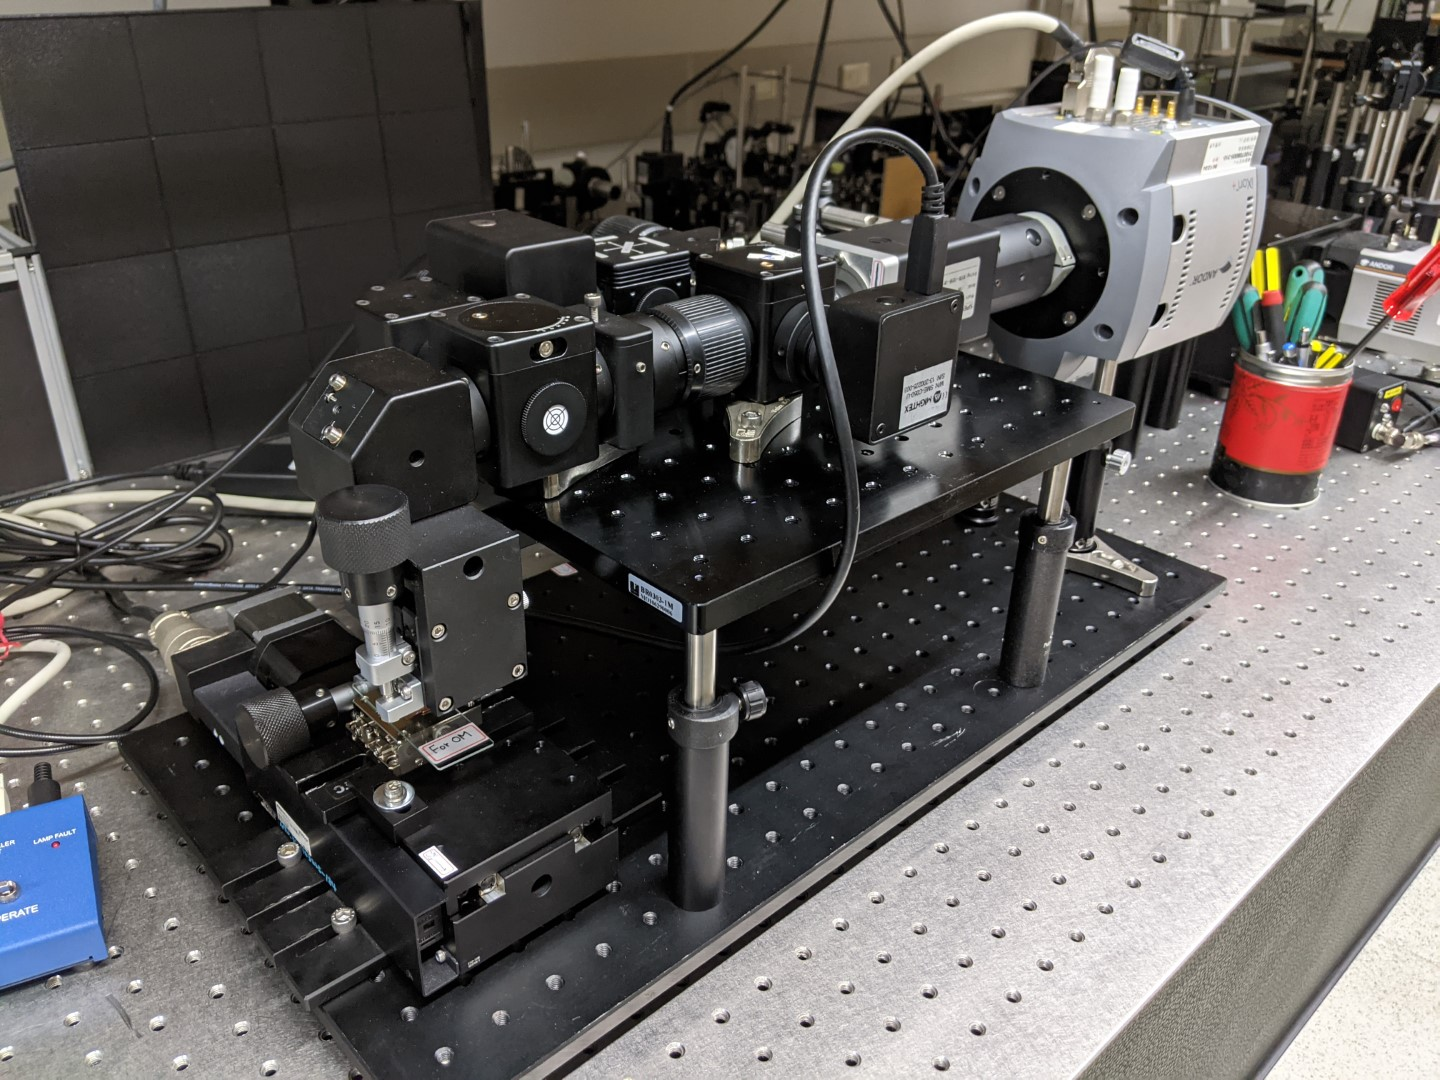
\includegraphics[width=\linewidth]{microSystemPixel3.jpg}
    \caption{Micro system.}
\end{figure}

\subsubsection{Galvo}
在最早的規劃中,第二階段的系統應該要從第一階段移動樣品的方式,改成以Galvo進行移動光源的方式掃描,但經過評估後,發現Galvo的運作方式並不適合線掃描系統。Galvo掃描的原理,是改變雷射點光源照射在樣品上的位置,
以一一對樣品上各個位置進行光譜量射。由於線掃描方式一次至少要將樣品上的整條掃描線完整照明,若以Galvo調動點光源的位置,則代表需要將光源在曝光時間內完整掃描一次樣品上的掃描線,並將掃描線上不同位置的像對應到狹縫上的不同位置。
然後,這樣勢必代表仍必須以電動載台移動樣品,才能將樣品上不同位置的掃描線之影像成在固定位置的狹縫上,如此的作法與現階段以面光源照滿光學顯微鏡視野,並移動載台的方式,並無效率上的優勢,
且以面光源照明尚有照明視野更大的優點。雖然以點光源方式理應可以相同的光源提供更強的照明,但在系統開發過程中亦沒有遇到照明強度不足的問題,因此就沿用第一階段以電動載台移動樣品的掃描方式。
\subsection{照明}
本系統現階段的照明設備,分別是高頻寬的Energetic LDLS與405 nm的DPSSL Laser,從兩個光纖collimator進入系統。照明光路的目標是希望能進樣擴大照明範圍,並使照明盡量均勻。
然而在系統架設的初期,energetic的照明存在明顯的上下不均勻現象,如圖與圖的比較所示,圖是初期進行光陸校正時使用的HL-2000光源照明下的影像,可以看見將同樣的光纖接頭改接LDLS光源後,照明變得非常不均勻。
且視野上下幾乎已經超出照明範圍。請這些都是在確認照明光路經過校正後的影像。
\begin{figure}
    \centering
    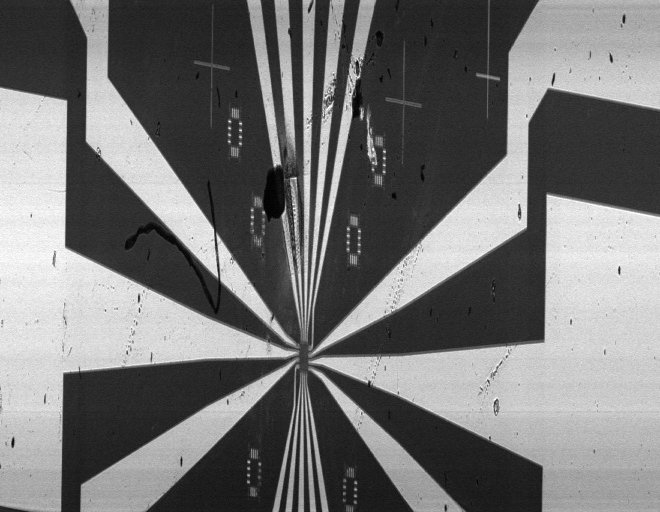
\includegraphics[width=0.5\linewidth]{0831focusForOmFullScanHL2000Scaled.jpg}
    \caption{HL-2000}
\end{figure}
\begin{figure}
    \centering
    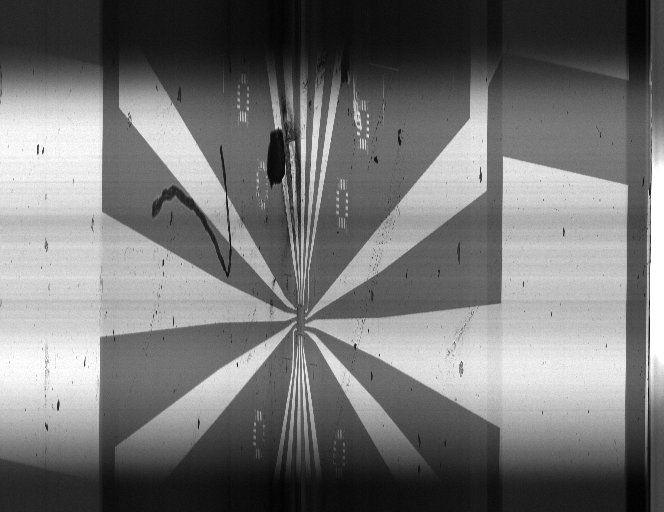
\includegraphics[width=0.5\linewidth]{0909Energetic.jpg}
    \caption{Energetic}
\end{figure}
為了改善照明的範圍,我們首先將原本使用的12.5cm tube lens換成現在所使用的15cm tube lens,希望能更集中使用成像中間較亮的部分,不過改善的效果有限,且系統上也沒有空間再裝設焦聚更長的透鏡。
為了要進一步改善照明的均勻度,我決定嘗試調整LDLS光源系統內,光線進入光纖的Coupler,以及光線離開光纖,進入影像系統的Collimator。經過多次嘗試後,最終得出三種組態,可以藉此瞭解前述兩個組件對於照明的影響。
\subsubsection{最高亮度、匯聚於背焦面} \label{section: illuOriginal}
簡言之,平移調整光線進入光纖的Coupler,會決定LDLS的照明光譜中進入光纖的波段。該Coupler原先的狀態,是調整至照明亮度最高,也可視為是最寬的頻寬進入光纖的狀態。
而光線離開光纖,進入照明系統的Collimator,即是一個可前後調整的透鏡,則會決定照明光源在影像系統內的何處匯聚。原先是調整至會剛好使照明光源正好匯聚在顯微物鏡背焦面的位置,使打在樣品上的光線為平行光。
在這個設定下,掃描所得的影像如圖\ref{figure: brightest_on},可以看到影像上下明顯較暗,表示照明範圍還不夠大。從圖\ref{figure: om_brightest_on}的彩色OM影像可以看到,照明光源有類似色相差的情形出現,
照明光源的影像不完整,且顏色也有分布偏移的情形。不過整體的照明尚算均勻,沒有明顯的干擾。
\begin{figure}[t]
    \centering
    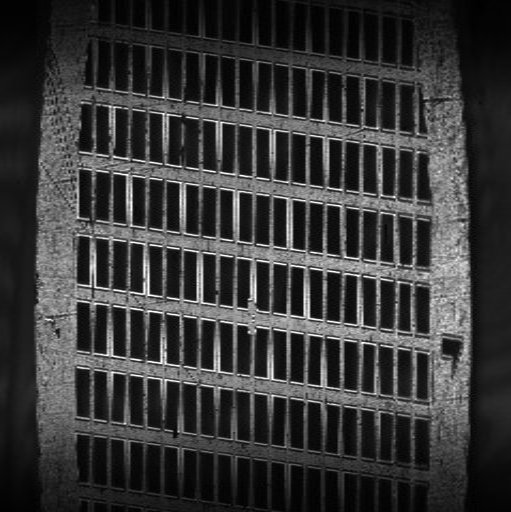
\includegraphics[width=0.5\linewidth]{on_brightest.jpg}
    \caption{Coupled at brightest, collimated on BFP.}
    \label{figure: brightest_on}
\end{figure}
\begin{figure}[t]
    \centering
    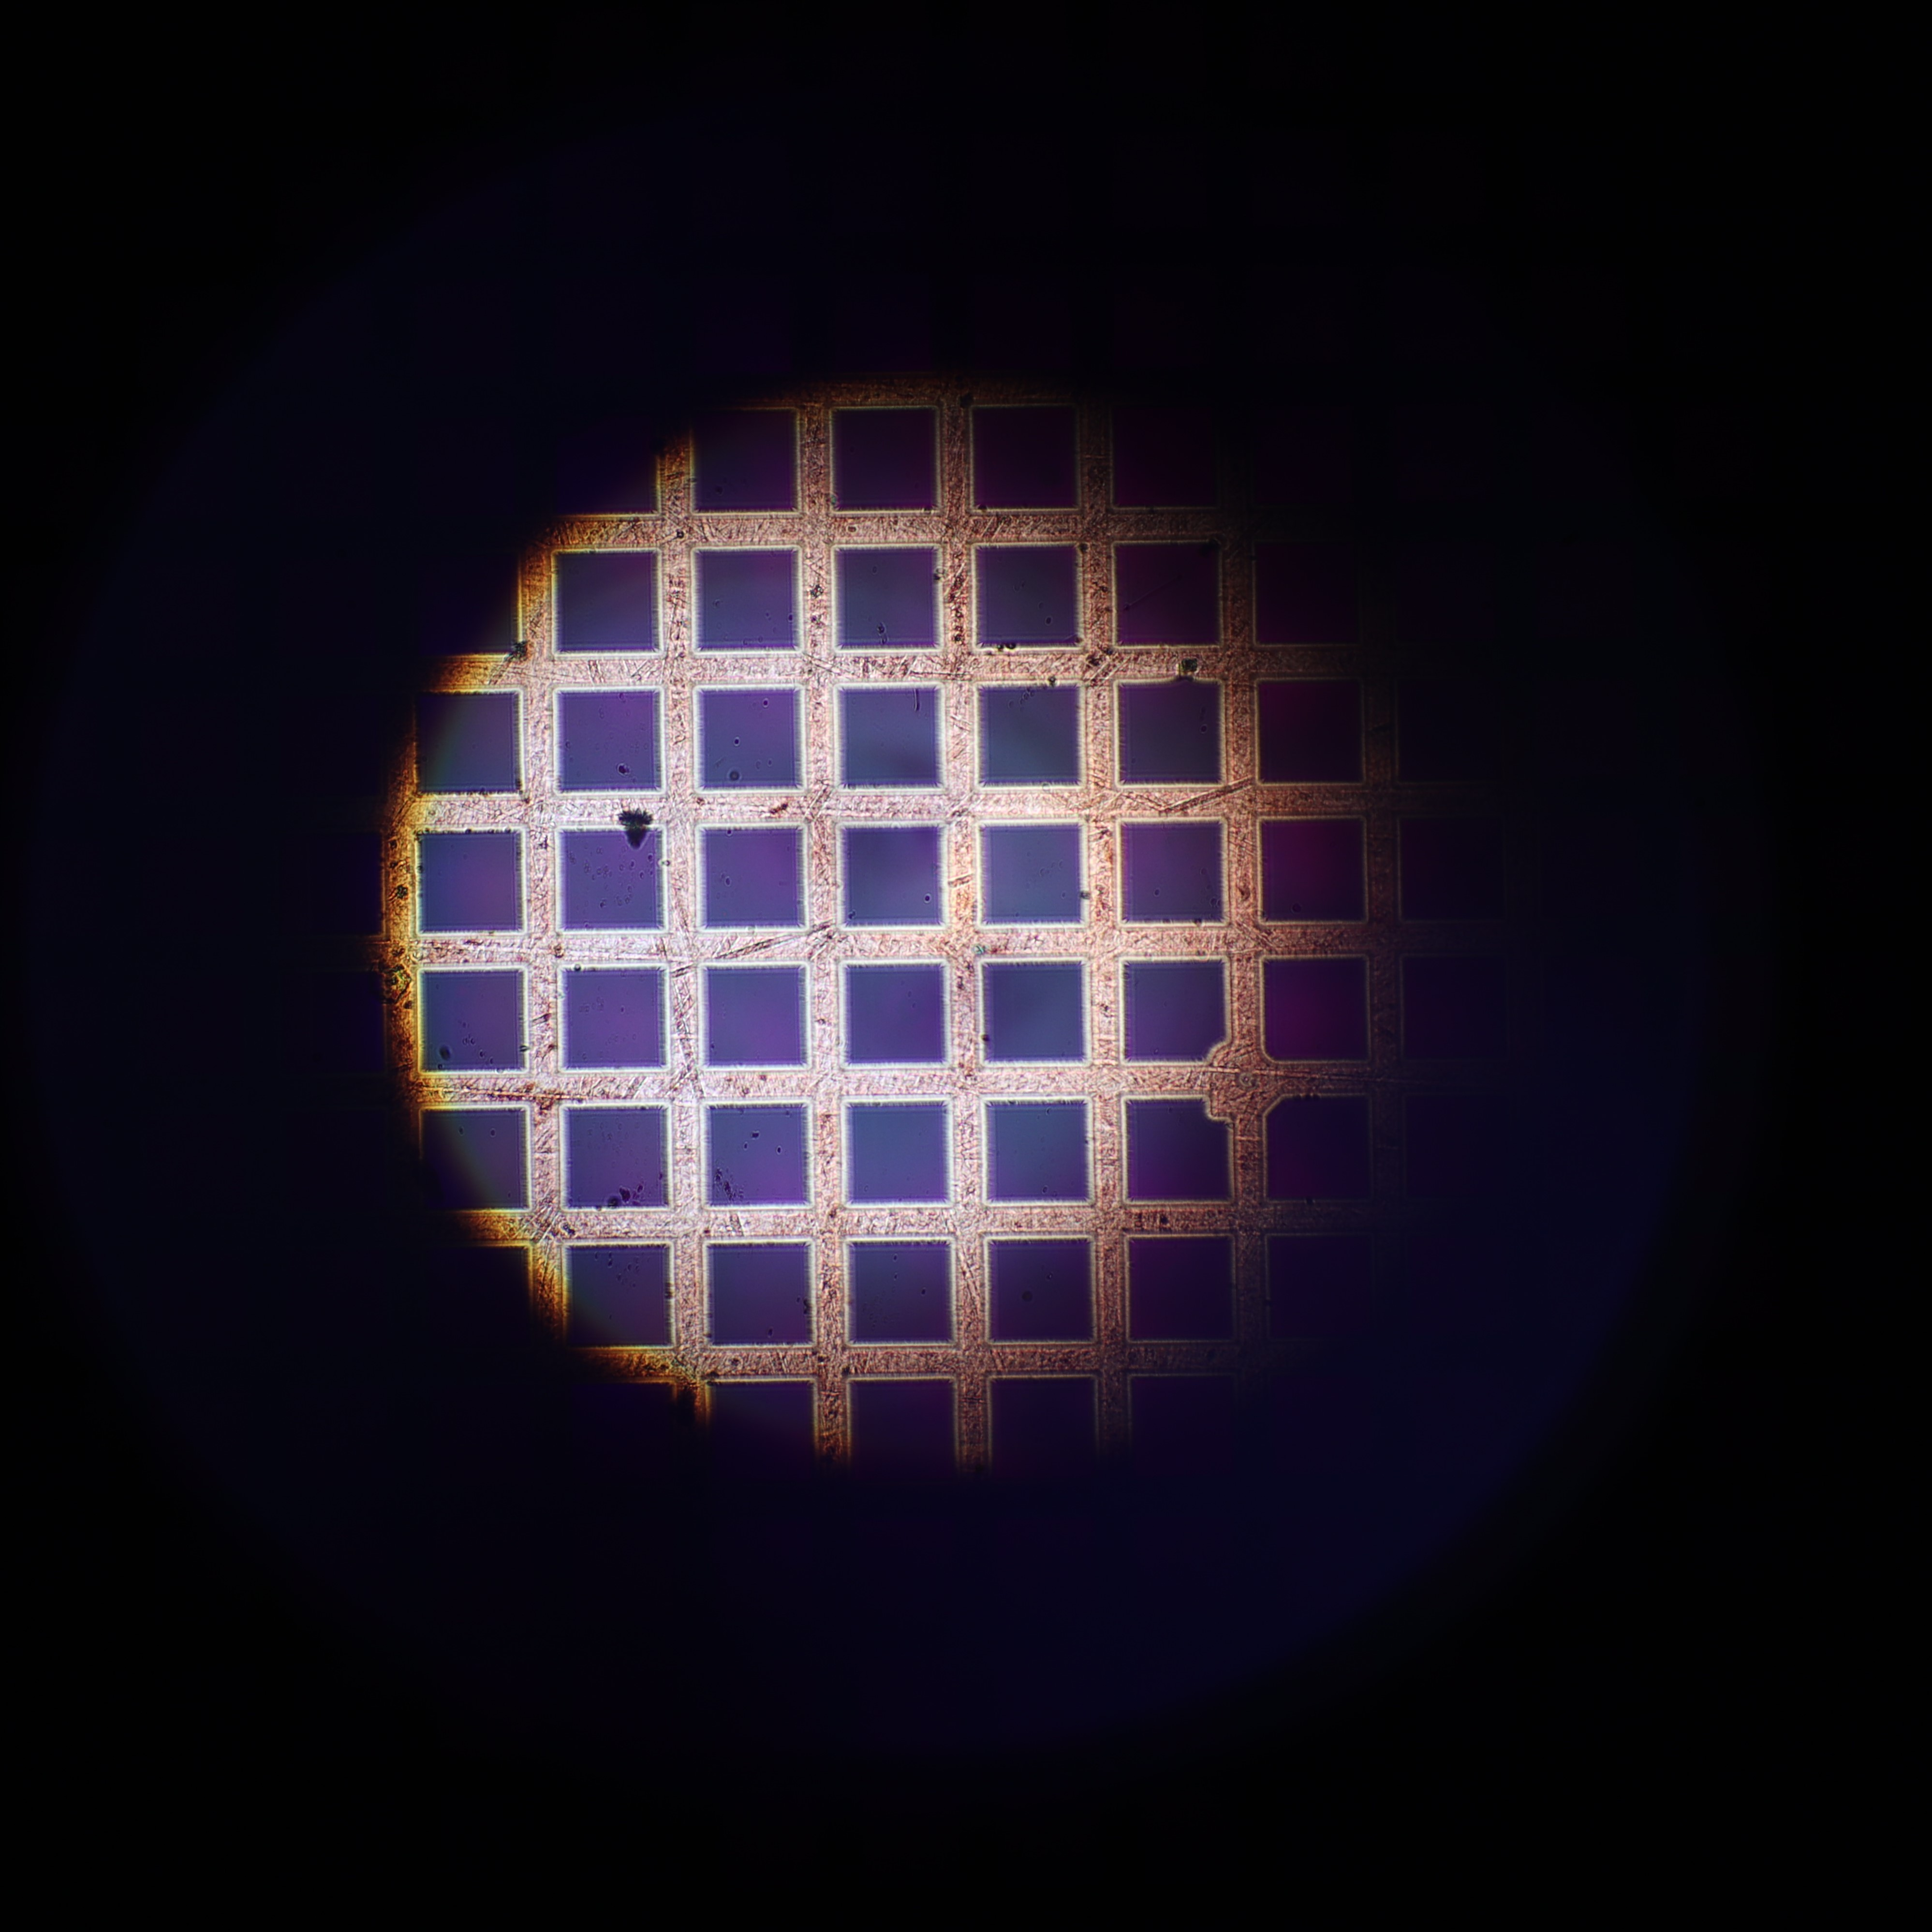
\includegraphics[width=0.5\linewidth]{om_on_brightest.JPG}
    \caption{OM: Coupled at brightest, collimated on BFP.}
    \label{figure: om_brightest_on}
\end{figure}
\subsubsection{最高亮度、不匯聚於背焦面}
從前述的設定開始做調整,若將Collimator稍微調動,使光源不要匯聚在顯微物鏡的背焦面上,可以把照明的範圍再做擴大,並完整的照滿整個物鏡視野,如圖\ref{figure: brightest_off}、\ref{figure: om_brightest_off}所示,影像不再有上下明顯的暗帶。由於光線並未匯聚於物鏡的背焦面,打在樣品上的光線並非平行光,
因此容易產生干擾的照明圖樣。以該螢光便樣品為例,由於螢光片半透明且具有厚度,不平行的光線穿過螢光片後,經反射後會產生不均勻的照明圖樣。
\begin{figure}
    \centering
    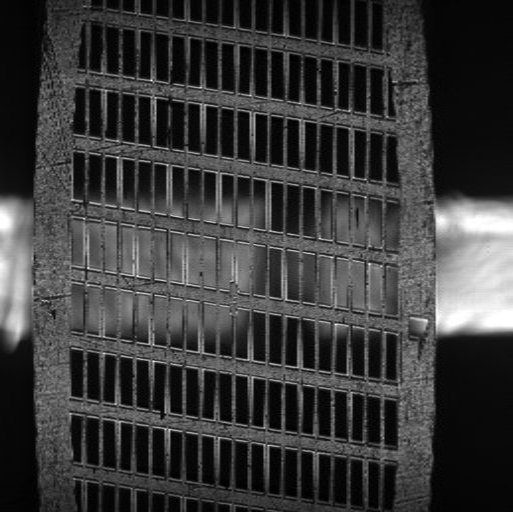
\includegraphics[width=0.5\linewidth]{off_brightest.jpg}
    \caption{Coupled at brighest, collimated off BFP.}
    \label{figure: brightest_off}
\end{figure}
\begin{figure}
    \centering
    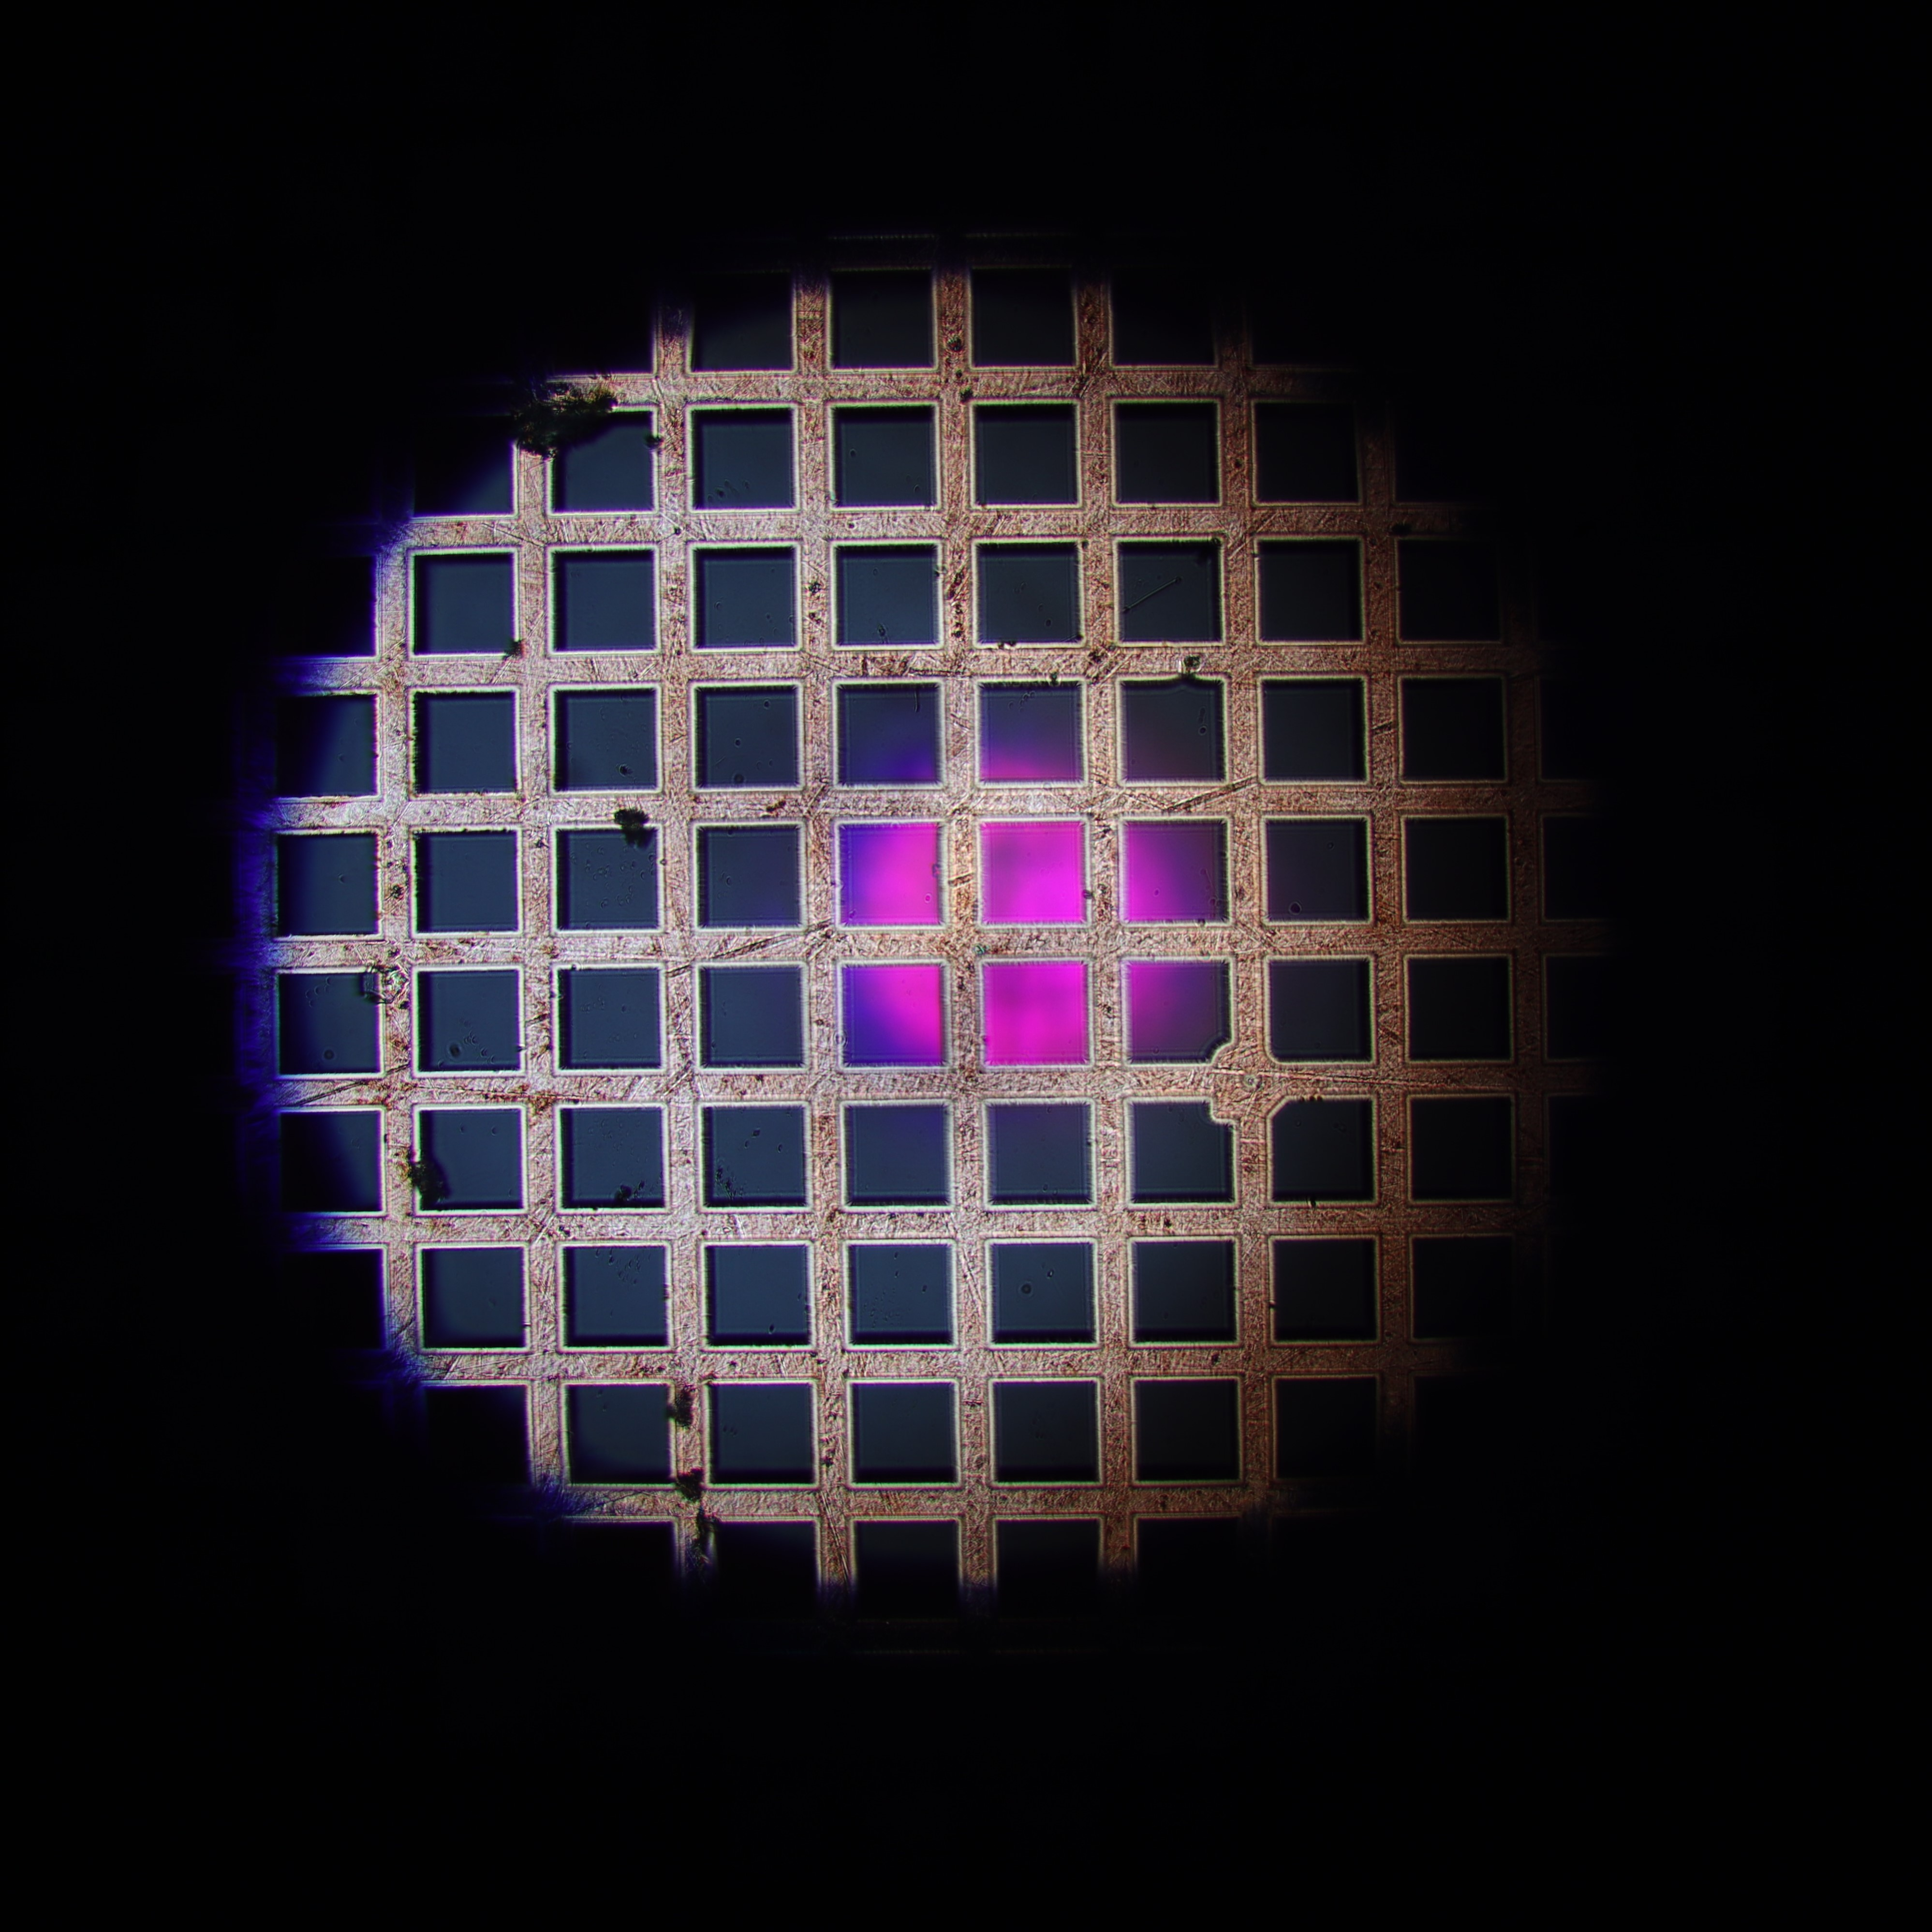
\includegraphics[width=0.5\linewidth]{om_off_brighest.JPG}
    \caption{OM: Coupled at brighest, collimated off BFP.}
    \label{figure: om_brightest_off}
\end{figure}
\subsubsection{較低亮度、匯聚於背焦面} \label{illuDark}
為了避免上一個設定方式明顯的干擾紋路,我重新調整Coliimator,將光源匯聚至物鏡背焦面,並改為調整光纖的Coupler,以解決原初的設定中照明範圍不足的問題。在圖\ref{figure: evenest_on}、\ref{figure: om_evenest_on}中可以看見,
經過調整後,照明關線的頻寬大幅減少,原先在\ref{section: illuOriginal}節中色相差的問題,幾乎完全消失,因此也確實可以完整的照明整個視野範圍,但由於實際進入光纖的光線已經減少許多,因此影像的整體亮度已有明顯的下滑。
\begin{figure}
    \centering
    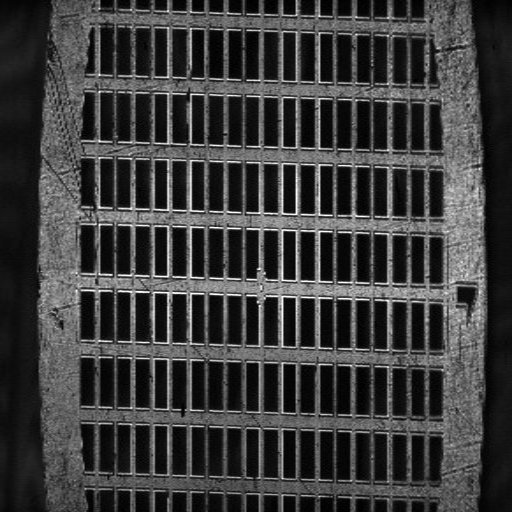
\includegraphics[width=0.5\linewidth]{on_evenest.jpg}
    \caption{Coupled at evenest, collimated off BFP.}
    \label{figure: evenest_on}
\end{figure}
\begin{figure}
    \centering
    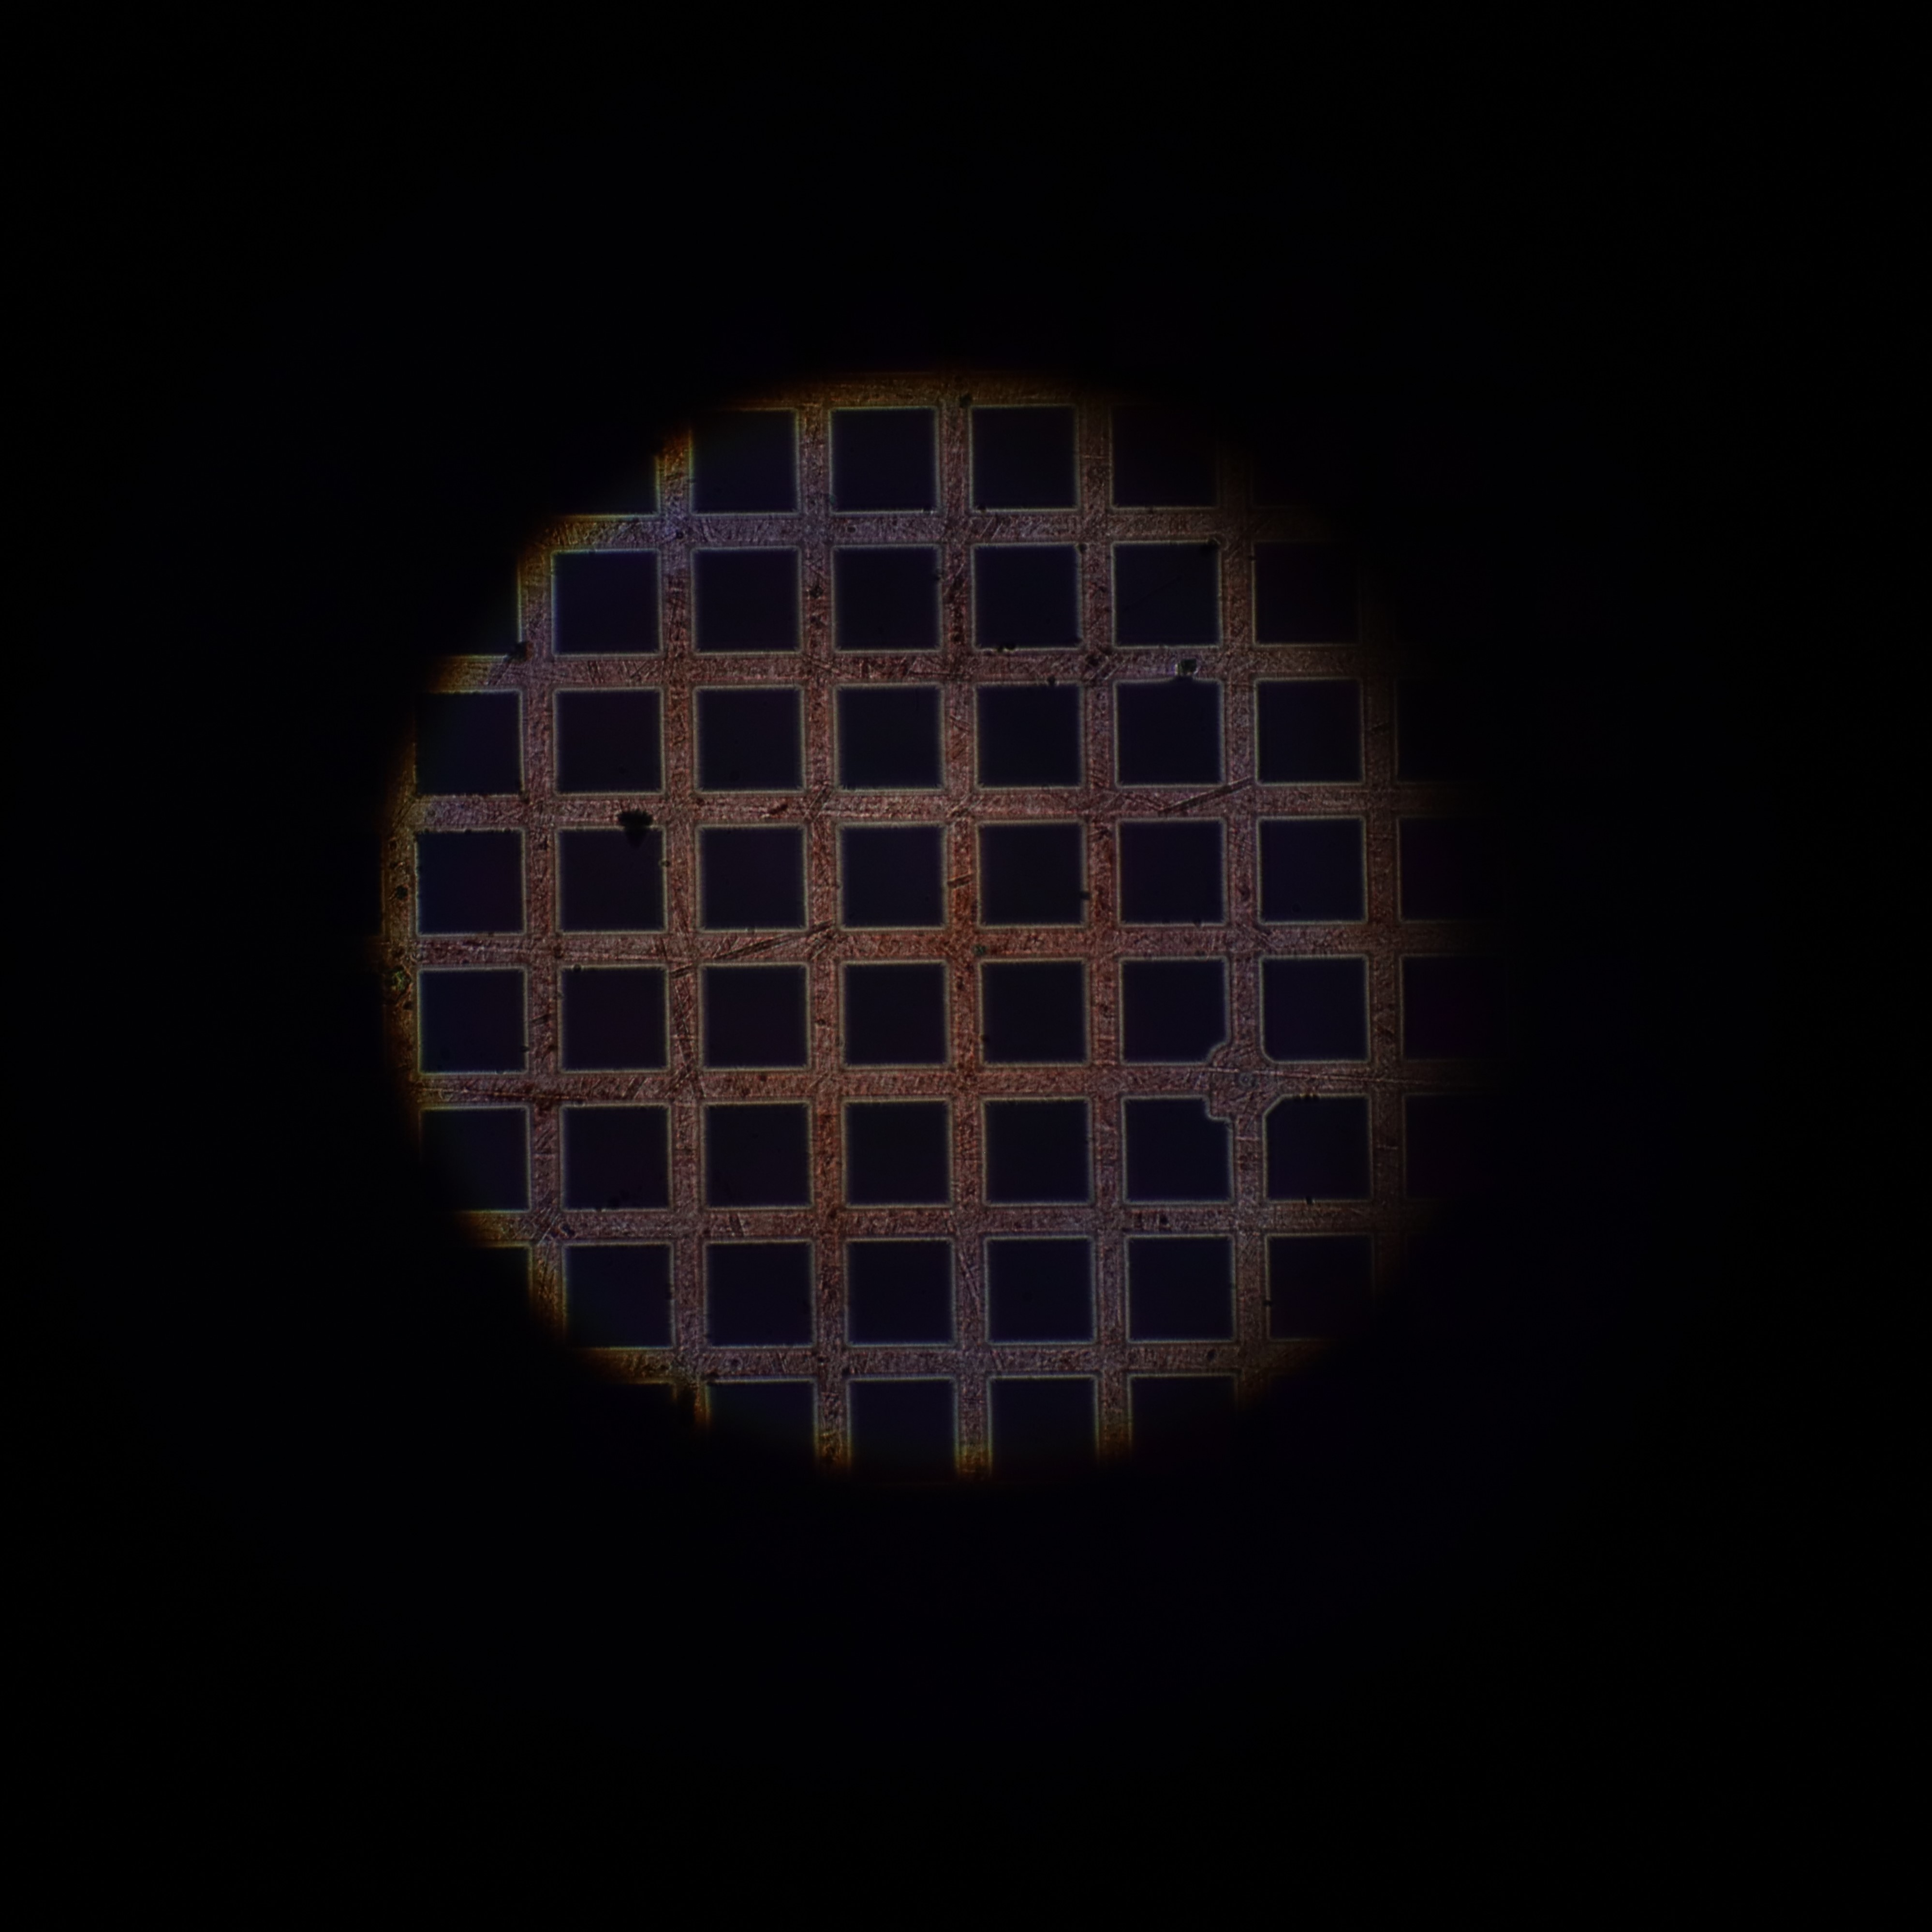
\includegraphics[width=0.5\linewidth]{om_on_evenest.JPG}
    \caption{OM: Coupled at evenest, collimated off BFP.}
    \label{figure: om_evenest_on}
\end{figure}

\noindent 綜上所述,照明的設定可以說是在光源光譜的完整度(頻寬)與照明範圍中做取捨,我們最後決定採取\ref{section: illuOriginal}節中的設定方式,
雖然照明最後所得的影像會在上下有明顯的暗帶,但情形不算特別嚴重,且可以透過軟體進行後期處裡。若為了排除下上較暗的問題,而採取\ref{illuDark}的設定方式,形同於浪費了LDLS光源系統多數的光譜頻段,
相形之下比上下的邊緣暗帶是更為嚴重問題,且也與我們因為需要更高頻寬的白光而使用LDLS的初衷背道而馳。

\subsection{.init檔}
軟體的.init檔案,目標是將一些重要的參數,如系統的影像大小、xyz三軸的校正等,儲存在一個可以更改的文字檔案中,當系統的硬體有更動時,只要調整該.init檔案內的參數值,軟體就可以做出相應的改變,
例如依據不同的影像尺寸進行記憶體的控管等。換句話說,透過init檔案儲存系統參數,就可以讓同一套軟體適用於不同的硬體上,只要檔案內的參數經過相應的調整即可。

本系統的init檔共分為五個區段,分別儲存系統視野、iXon、電動載台、光譜校正與OM相關的參數。軟體在啟動時會將這些參數一次讀取,並儲存到相應的run-time變數中,以方便隨時取用。
我們使用的檔案語法是LabVIEW內建的Configuration file VIs所產生的標準init檔語法,其易於閱讀的特性,讓使用者可以直接透過一般的文字編輯器進行修改。其中某些參數,也會在軟體操作過程中由軟體自行做合適的修正。

關於.init檔案的詳細使用說明,與每個參數所代表的意義和用處,請參閱本系統的.init檔說明文件(.init file documentaion of HSI system)。
\subsection{軟體結構調整}
隨著程式的軟體功能漸趨完備,操作上越來越複雜,各個功能所需的程式碼也都會佔去龐大的空間,使的程式碼的原檔變得過於冗長,變得非常難以閱讀與偵錯。且許多會重複使用、或是功能相近的程式碼也浪費了不少空間。
另外,許多資料或變數必須在程式的不同區塊間傳遞,常常需要拉很長的資料線路(LabVIEW data wire),容易造成資料流變得混亂。為了改善這些問題,並使後續更進階的軟體功能開發更加便捷,我們決定將程式進行大規模的改造,將程式碼全部模組化,
主程式只控制UI與執行模式,其餘功能皆以函式呼叫(LabVIEW subVI)來達成。另外,也更廣泛的以各種LabVIEW變數(LabVIEW local variable、global variable、functional global variable, FGV)來儲存並傳遞資料,使程式的
資料流變的清楚明確。

將程式完全模組化後,主程式的檔案尺寸縮減至一半,整體的程式碼也變得更加整齊、一目瞭然。在前端使用者介面完全不變的情形下,這些sunVI之間的API需要經過不少設計與調整,
才能確保基本的運作都能以正確的參數完成。我們也使用了許多control reference的傳遞,來使subVI能夠直接控制主程式上的使用者介面,這樣的操作方式減少了許多不必要的資料流,在整個模組化的過程中相當重要。
我們也同時順便確立了程式的執行流程,在原始碼更易讀的情形下,更容易看出程式目前的所在階段,對於UI要因應不同階段做出改變,也很有幫助。

在資料流的精進部分,主要透過以下三種方式來達成:
\begin{enumerate}
    \item 若是主程式內的UI相關資訊,例如使用者的滑鼠點擊位置,就以本地變數(local variable)來儲存,以方便主程式內不同的event catcher或不同模式的程式取用資料。
    \item 若是.init檔或是影像擷取設定相關的資料就以專案全域變數(project global variable)的方式儲存,如此一來每一個subVI都可以自行對同一個變數進行讀取,能夠簡化API的設計。
    \item 最主要的影像資料data cube,則以一個functional global variable儲存,主要的原因是三維影像資料的數據較多,若以傳統的全域變數方式儲存,每次讀取時資料都會被複製一次,造成記憶體的浪費。
          另外,FGV是本身可程式化的全域變數,除了可以對存取衝突的狀況進行處裡外,也方便做一些基礎的資料處理。
\end{enumerate}

\subsection{使用者介面與功能}
在軟體的前端介面上,我們希望讓使用者一目瞭然,能夠以最快的方式在螢幕上找到他所需要的控制項。因此將所有的控制按鈕分為數個類別,並從視覺上以背景圖塊(LabVIEW decorations)做出區別。
另外,為了避免介面整體太過雜亂,在控制項的造型上都選用LabVIEW中內建與Windows系統風格一致的system控制項系列。因此整體的畫面簡潔,且不會有過多且不必要的視覺元素干擾使用者對整體介面的理解,
僅輔以部分其他風格的UI物件(silver decorations)幫助使用者理解各類別控制項的分區,達到操作上直觀與美觀的目的。

除此之外,操作介面除了靜態上的設計外,也有許多會需要因應使用者輸入來進行回應的動態變化。首先是希望使用者所有的輸入都能得到介面上的反應,讓使用者知道操作是否成功。另外,也盡量使用一些視覺元素,例如表達系統冷卻情形的顏色、載台移動中的燈號、矩陣旋轉的進度條等,
來提醒使用者目前系統的狀態。這些動態的設計能避免讓使用者對於系統的操作狀態感到困惑。

接著,雖然介面上布局排版不會在操作過程中有重大改變,但許多文字、圖表標題、尺規,會隨著顯示的內容不同,做出相應的變化。而在當下不應該被使用的控制項,也會在視覺上明顯的被淡化,
從圖\ref{figure: acquire mode}與圖\ref{figure: scanning}的比較即可看到,進行掃描時所有的影像設定皆不應被更動,因此在介面上相關的控制項皆被淡化關閉。
\begin{figure}
    \centering
    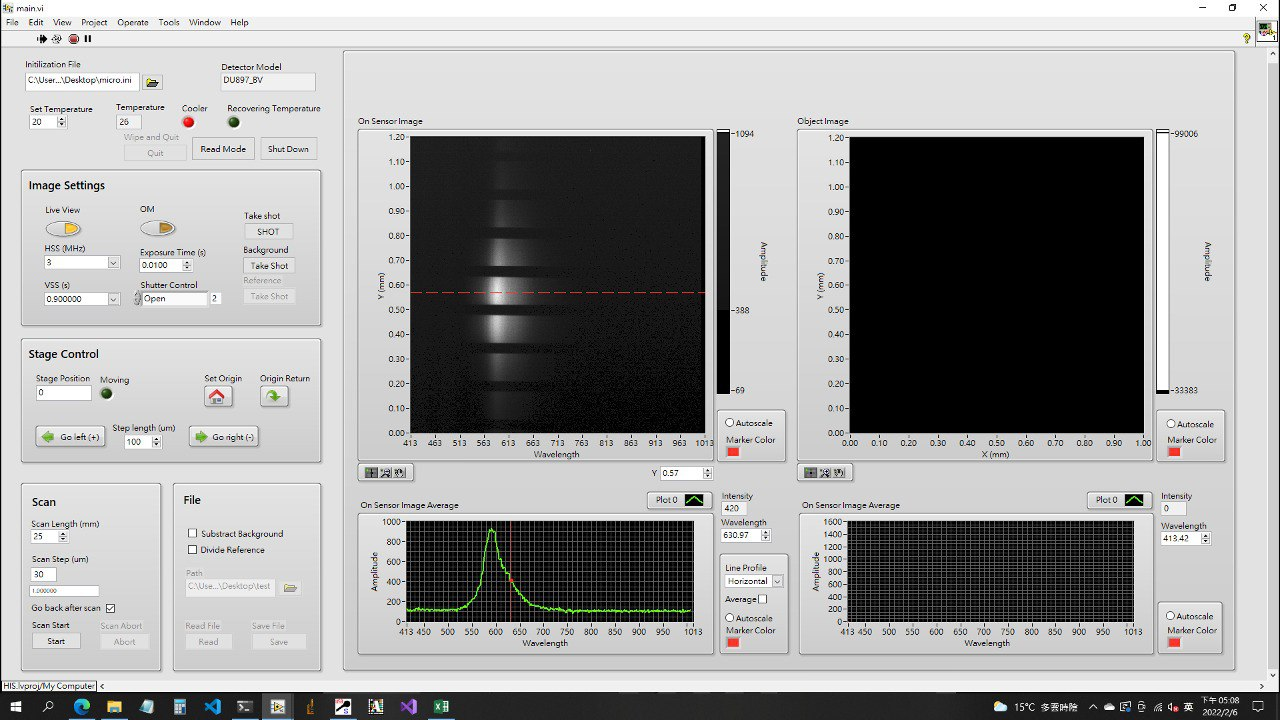
\includegraphics[width=\linewidth]{acquire.jpeg}
    \caption{在影像模式下的軟體介面。}
    \label{figure: acquire mode}
\end{figure}
\begin{figure}
    \centering
    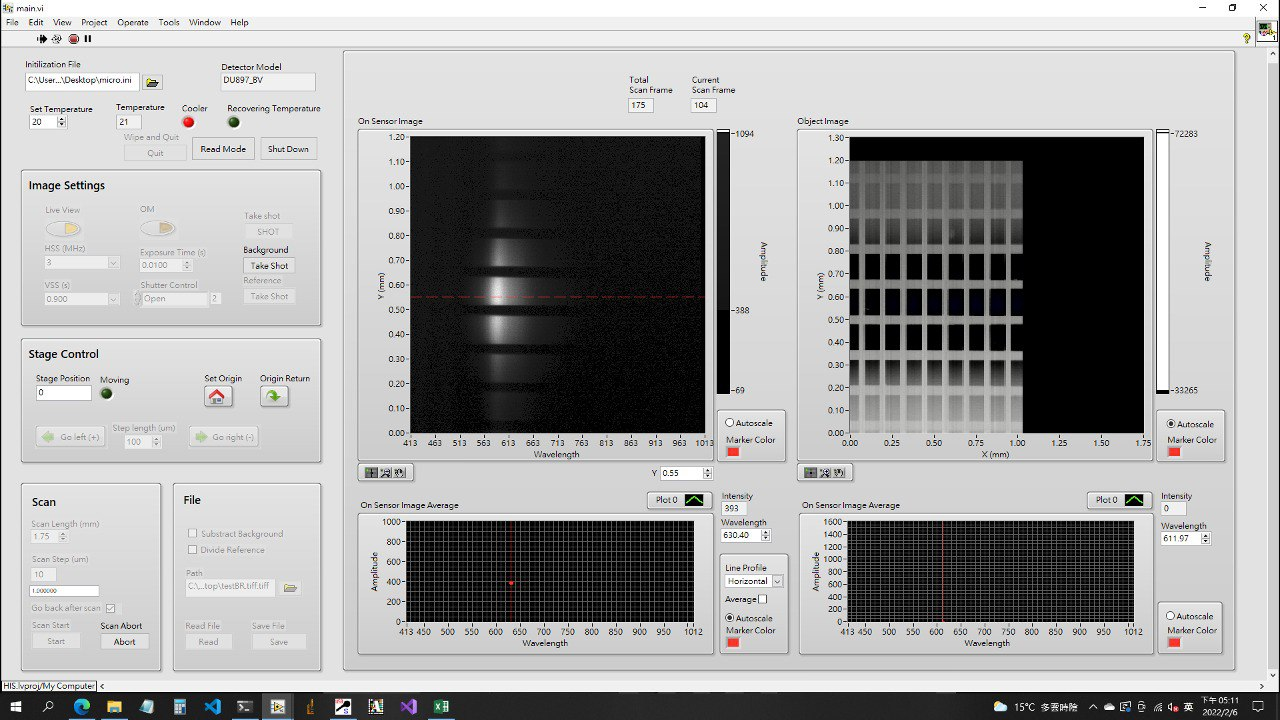
\includegraphics[width=\linewidth]{scanning.jpeg}
    \caption{掃描時的軟體介面。}
    \label{figure: scanning}
\end{figure}
\subsubsection{ROI框取}
本階段中重要的軟體功能開發之一,就是圖\ref{figure: roi}中的ROI框取功能。當使用者打開OM影像畫面後,可以透過下方的拉桿調整掃描起始與結束的位置,接著只要按下ROI Scan,系統就會自動完成範圍內的掃瞄。
該功能的開發過程中,最重要的是OM影像上所框取出的範圍,要如何轉換為實際的長度。為了完成這樣的校正,我們另外設計了一個校正用的程式,其可以讀取Canon 相機的影像,並在影像上讓使用者
畫上定位點,以計算樣品實際長度與螢幕顯示座標的比例關係。

除此之外,這個功能的開發,也牽扯到許多OM顯示的設計。由於我們並沒有使用到Canon M200影像感測器的全幅畫面,因此OM影像需先經過裁切,這些裁切的設定也都儲存在.init檔中,可以參考.init檔的OM章節。
同時還要在OM影像上顯示線分光儀當下所觀測的位置(圖\ref{figure: roi}中白色垂直虛線),以及線分光儀的Y軸視野範圍(圖\ref{figure: roi}中兩條白色水明虛線),這些都需要以校正程式與具有已知特徵的樣品來協助判斷,
\begin{figure}
    \centering
    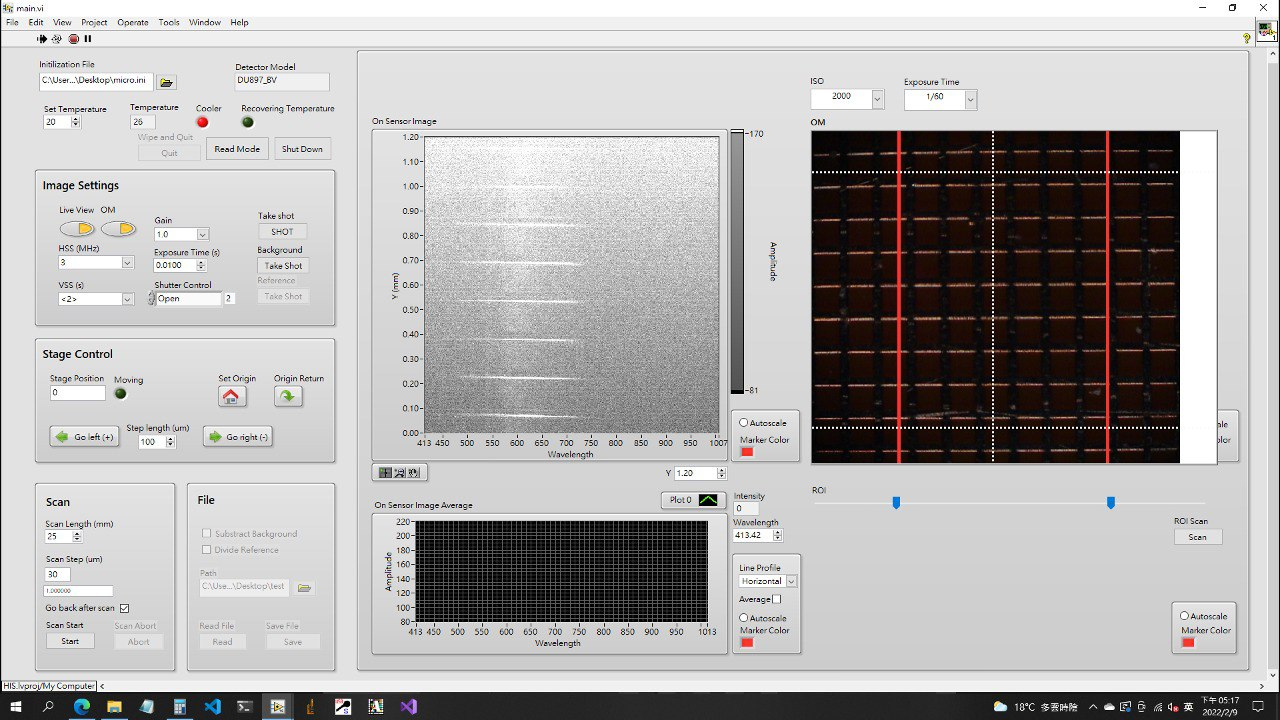
\includegraphics[width=\linewidth]{roi.jpeg}
    \caption{ROI框取功能。}
    \label{figure: roi}
\end{figure}

\subsubsection{背景/參考光譜}
由於本系統以平行光進行照射的特性,非常適合作反射光譜的量測。然而,量測反射光表示我們必須對光源在光譜或空間中的不均勻進行校正,換句話說,我們希望量測的是樣品在各波長下的反射率,而非光譜本身。同時,在多數的光譜量測中,我們也都必須對影像感測器的背景雜訊進行校正,
因而著手開發背景光譜(背景雜訊)與光源參考光譜的擷取與校正功能。實際進行校正時,是將背景光譜(雜訊)油源資料中減去,再除以參考光譜。在操作的介面上,由於背景光譜幾乎可以適用於所有類型的光譜量測,而參考光譜只需要用於反射光譜的量測,因此我將其設計為兩個按鈕,可以分別進行擷取。然而需要注意的是,根據反射率的計算式
\begin{equation}\label{equation: reflection}
    reflection \quad rate=\frac{measurement-background}{reference-background}
\end{equation}
若沒有擷取背景光譜,則參考光譜本身是無法用於校準的,因為參考光譜也必須減去背景雜訊後才能用於校準。因此介面的設計上,在沒有擷取背景光譜前,擷取參考光譜的按鈕將會是淡化且關閉的。

使用者按下背景光譜按鈕後,系統會關閉iXon的快門,以當前所設定的影像參數拍攝一張張片,並顯示於右側螢幕,再將快門恢復至原本的狀態。系統會記錄下目前已經有拍攝背景光譜影像,並將背景光譜影像儲存在另一個FGV中。
相似的,當使用者按下參考光譜的按鈕後,系統會開啟iXon的快門並以當前所設定的影像參數拍攝一張張片,該影像會被減去背景光譜\footnote{相減後數值小於0的矩陣元素會一律被設為0。},接著儲存到FGV中。

在高光譜影像掃描完成後,將影像資料data cube存進FGV中時,系統就會在FGV內進行相應的校準運算。由於軟體系統有以變數記下使用者是否有拍攝背景/參考光譜影像,因此掃描結束後,進行光譜瀏覽時,
系統即會顯示讓使用者選擇要瀏覽原始反射光譜影像或是校正後的反射率影像的選項。
\begin{figure}[ht]
    \centering
    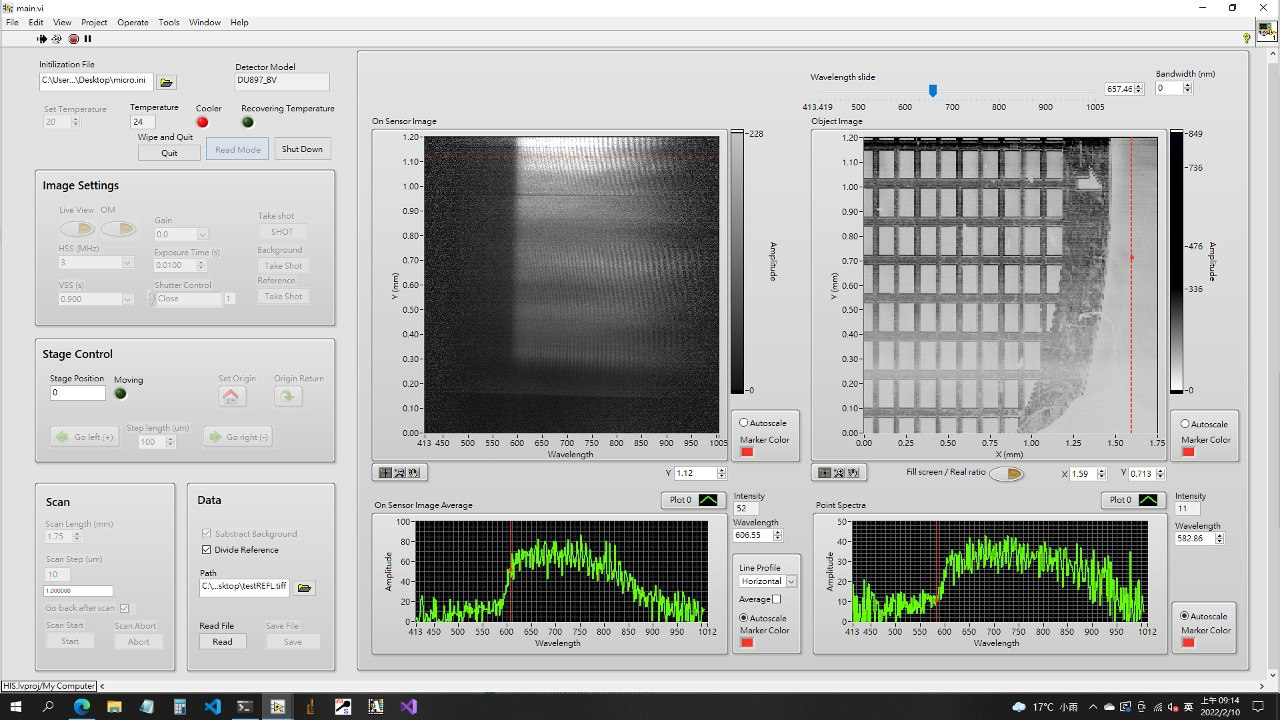
\includegraphics[width=\linewidth]{reflection.jpeg}
    \caption{檢視反射率影像時的軟體介面。}
    \label{figure: reflection}
\end{figure}

\subsection{第三階段: 功能優化}
由於第三階段的背焦面影像系統實際上只是在第二階段的系統上再加入被焦面成像的模組,因此本階段的開發主要先集中在系統各項功能的優化,並在軟體方面針對高光譜掃描影像的資料瀏覽與分析功能進行擴充,
以其整體系統整合的基礎功能完善且穩定,最後再針對被焦面影像系統的硬體與光路進行探討。

\subsection{掃描速度優化}
掃描速度的優勢是本系統採用線掃描技術進行開發的重要原因之一,本章節說明我們對系統掃描速度所進行的量測與優化過程。
\subsubsection{掃描迴圈}
為了要瞭解決定掃描速度的各個因素,首先要先說明整個掃描的行程是如何進行的。所謂掃描,其實就是在樣品的數個不同位置上以相同的參數拍攝線掃描影像,
在使用者設定好掃描範圍與掃描步進(也就是每條掃描線之間的距離),電腦軟體會執行以下的迴圈,控制iXon與電動載台進行掃描:\textbf{首先},將電動載台移動到欲拍攝線掃描影像的位置,
在每個迴圈中,這個移動的距離是固定的,也就是掃描步進。\textbf{接著},在確認電動載台已經移動到正確位置後,下指令使iXon開始擷取影像,確認iXon已經完成影像擷取後,iXon會將資料傳回電腦,
程式並會進入下一次迴圈,重複執行以上動作的次數,是由程式以使用者設定的掃描距離除以掃描步進進行計算。\textbf{迴圈次數執行完成後},電腦會將每條掃描線上所取得的線掃描影像接合成三維矩陣,
為了確保該三維矩陣的「正面」是如肉眼所見的樣品影像,該矩陣還須經過旋轉,此矩陣旋轉的過程也需要時間。

以下對於掃描時間的討論,皆是以一掃描範圍長3.5mm,掃描步進$10\mu m$(也就是總共拍攝350張線掃描影像並接合),曝光時間10ms的高光譜影像掃描為例。為了瞭解其他各項影像參數(HSS, VSS)對於掃描速度的影響,
我調整iXon的HSS, VSS進行拍攝,並量測不同組合下所有迴圈執行完成所需的時間、迴圈執行後矩陣建立與轉向所需的時間,並以LabVIEW的precision timer(High Resolution Relative Seconds.vi)量測影像擷取完成後傳輸到電腦所需的時間。
在以下的測試中,整個掃描迴圈中有三個等待時間,分別是等待電動載台移動至定點的時間,另一是等待iXon影像擷取完成的時間,以及等待iXon將資料傳輸到電腦所需的時間。這三個等待時間的設定方式如下所述:
\begin{enumerate}
    \item 等待電動載臺: 電腦將電動載台移動的指令傳輸給電動載台控制器後,會等待\begin{equation} \label{eq: stageWait}
              \text{掃描步進}\times 200 \div 750 \quad milliseconds
          \end{equation},再進行迴圈內的下一個動作。
    \item 等待iXon擷取影像資料: 電腦在下指令給iXon進行影像擷取後,以一個while loop每1.5倍的曝光時間就詢問一次iXon的狀況,直到iXon回報擷取已完成後,才會進入迴圈內的下一個動作。
    \item 等待iXon傳輸影像資料: 電腦會等到「讀取iXon影像資料」的程式全部執行完成後,才會繼續迴圈內的下一個動作。
\end{enumerate}
再以上的設定下,所進行的測試結果如表\ref{tab: measuring}所示,表中的Pull sum代表350次迴圈中\textbf{等待iXon傳輸影像資料}所需時間的和,
$t_1$代表350次迴圈執行所需的總共時間,$t_2-t_1$則是代表掃描結束後矩陣接合與轉換所需的時間。該表格的測試提供了以下資訊,首先,若HSS頻率設定為1/3,掃描所需時間幾乎也會正好三倍,
相對的,VSS對掃描的速度影響較小。HSS與VSS對於iXon運作的影響,可以參考iXon說明書的附錄。\cite{ixonManual}
接著,\textbf{等待iXon傳輸影像資料}所需的時間極短,每張照片約1-2 milliseconds。最後,矩陣接合與轉換的時間雖然只與電腦的效能有關係,但所需的時間可能會占總掃描時間的將近1/3。
\begin{table}[]
    \centering
    \begin{tabular}{lll||llll}
        HSS   & VSS & Expo & Pull sum & Scan $t_1$ & $t_2$   & $t_2-t_1$ \\ \hline \hline
        3     & 0.9 & 0.01 & 554      & 44.1       & 01:28   & 43.9      \\ \hline
        3     & 1.7 & 0.01 & 502      & 45.25      & 01:10.1 & 25.55     \\ \hline
        3     & 0.5 & 0.01 & 581      & 43.76      & 01:09.7 & 25.94     \\ \hline
        1     & 0.9 & 0.01 & 497      & 01:48.9    & 02:20   & 71.1      \\ \hline
        1     & 1.7 & 0.01 & 633      & 01:50.0    & 02:16.2 & 26.2      \\ \hline
        1     & 0.5 & 0.01 & 588      & 01:48.7    & 02:13.9 & 25.2      \\
        (MHz) & (s) & (s)  & (ms)     & (mm:ss)    & (mm:ss) & (s)
    \end{tabular}
    \label{tab: measuring}
    \caption{影像設定對掃描時間的影響。}
\end{table}
\subsubsection{速度提升}
為了要使掃描的速度進一步加快,我們決定從前述的三個等待時間開始進行優化。首先,在前述的測試中已經顯示出,第三項\textbf{等待iXon傳輸影像資料}所需的等待時間極短,並不是決定掃描速度的關鍵因素。
因此以下將集中討論\textbf{等待電動載臺}、\textbf{等待iXon擷取影像資料}兩個等待時間的調整。
\subsubsection{電動載臺等待時間}
原先用來計算電動載台等待時間的算式\ref{eq: stageWait},在進行掃描時被發現可能會有等待不足就下指令給iXon進行拍攝的問題,因此改以一個while loop,在下指令給電動載台控制器後,不斷詢問電動載台目前的狀況,
直到控制器回報電動載台已經停下後,程式才跳出while loop並繼續下一個動作。然而,這樣的等待方式會造成掃描速度在各項設定下大致都變成表\ref{tab: measuring}的三倍,雖然最為保險,但其速度較難令人接受。
最後,我們將電動載台的Drive speed (F)、acceleration/deceleration speed (R)、Startup speed (L)皆設為400,並且計時載台移動固定距離的時間,發現電動載臺確實是以400 pulse per seconds(pps)的速度前進,
即可以此數值準確計算每次載台移動所需的等待時間,實務上,我還加上了10ms做為緩衝。
這樣的設定方式再開發與使用過程中皆沒有遇到等待不足的問題,且掃描時間也大致回復到表\ref{tab: measuring}中的速度。
\subsubsection{iXon擷取影像資料的等待時間}
如前所述,這段等待時間是以while loop不斷詢問iXon的方式決定,經過LabVIEW的precision timer量測後,發現以這樣的方式操作,在350張影像的掃描中,以表\ref{tab: measuring}第一列的參數設定,
平均每張影像需要0.13213 seconds的時間iXon才會回報擷取完成。為了要減少這段等待時間,我們翻閱Andor SDK的說明書,希望能找到更快確認iXon影像擷取完成的方法,再經過各項嘗試後,
我們發現用來控制iXon的程式庫Andor SDK中的GetAcquisitionTiming函式,所傳回的最低影像擷取等待時間,也高達0.117 seconds。而我們最終所採用的方式,是以Andor SDK的Wait Acqusition
函式來等待影像資料擷取,並且設定iXon只讀取CCD上我們會使用到的區域(參見圖\ref{figure: image size}),最終以LabVIEW的precision timer量測,等待時間減少至0.10662 seconds。

\subsubsection{矩陣接合與旋轉}
原先可能需耗費40秒進行的矩陣運算時間,在改以LabVIEW 的loop parrallelism操作後,能夠減少至約7秒的時間就完成。\footnote{不過該耗時仍與電腦的效能高度相關,實測在一樣的設定下,有可能僅需3秒即完成。}
在經過以上的各式調整後,同樣進行350張線掃描,掃瞄範圍3.5mm,以0.01秒的曝光時間、0.9 HSS、3MHz VSS,掃描時間$t_1$正好為一分鐘,另約需4秒進行矩陣轉換,總計1:05即可完成掃描,並開始進行觀測。

\subsection{影像檔案讀取與進階存檔}
\subsubsection{檔案讀取}
本系統軟體截至目前為止皆以掃描功能為核心進行開發,只有在掃描結束後能對掃描的資料進行瀏覽,存檔並關閉後只能使用其他軟體來瀏覽掃描資料。為了讓使用者能有便捷的界面對過去掃描的資料進行瀏覽,我決定以
原有的瀏覽介面,直接加上讀取檔案的功能。在開發上,讀取檔案的程式碼並不複雜。由節\ref{section: saveTiff}所述可知,Tiff檔案由影像資料標籤,與影像資訊本身組合而成。讀取Tiff檔案的方式相當直觀,
首先讀取影像資料標籤,並透過影像資料標籤得知影像在檔案中的位置與大小,再讀取影像本身。不過由於我們所採用的為經過擴充之後的Tiff檔案,除了有公版的Tiff標籤外,尚有其他實驗室自行開發的軟體會需要的標籤,
這些標籤分別儲存在兩個影像資料索引中(Image File Directory):公版IFD與實驗室的ULS IFD\footnote{IFD基本上就是將一群用途相似的影像資料標籤放在檔案中的相鄰位置,組成一個影像資料標籤的群組。},
整體讀檔的操作順序大致如下所述。
\begin{enumerate}
    \item 檔案起始處,跳過位元端序宣告\footnote{讀取檔案時理應先確認檔案寫入的端序設定,但由於本系統寫檔時一律以little-endian方式,因此讀檔時也一律採取little-endien設定,故不再讀取檔案起始處的端序宣告。}等數個位元組後(請參閱原始碼),即是公版IFD,從此處開始讀取基本的影像資料標籤。
    \item 因為每個影像資料標籤的大小皆為固定的12位元組,從此處開始每12個位元組即為一個影像資料標籤,依序讀取即可。
    \item 每個影像資料標籤皆依序包含:2個位元組儲存其ID(一個U16數字)、2個位元組儲存其檔案類型、4個位元組儲存其數量,剩下4個位元組儲存標籤資料本身。依此方式,即可讀出影像資料的ID,從前述.xlsx檔案即可對照出其意義,接著讀資料檔案型態後,即可以相應的方式將其最後幾個位元組的資料unflatten出來。
    \item 公版影像資料標籤中,有一個標籤是實驗室IFD的位置,從這個位置資訊即可以相同方式讀出所有必須的影像資料標籤。
    \item 公版影像資料標籤中,另有一個標籤是影像資料的位置(image strip offset),透過該位置資訊即可知道影像資料的位置,並存其他影像資料標籤計算出其大小,直接到該位置將正確大小的資料unflatten為正確大小的三維I32矩陣,所得的矩陣就跟剛掃描完時的矩陣擁有相同的性質,可以被原本的軟體直接讀取。
\end{enumerate}

有時使用者開啟軟體,僅是需要讀取檔案並瀏覽光譜,此時可以點按進入Readout Mode,系統即會跳過軟體的影像設定與掃描程序,直接進入瀏覽模式。
另外,系統軟體開啟時,會自動啟動iXon的Andor SDK與Canon EDSDK,軟體會透過這兩個外部程式庫的執行錯誤來判定軟體系統是否有成功與硬體系統連接,並跳出視窗提醒使用者,同時也會避免對沒有連接的硬體系統下達指令,以避免更多錯誤產生。
若軟體偵測到系統的主要影像感測器iXon沒有連接上,即會自動進入讀取模式。
\begin{figure}[ht]
    \centering
    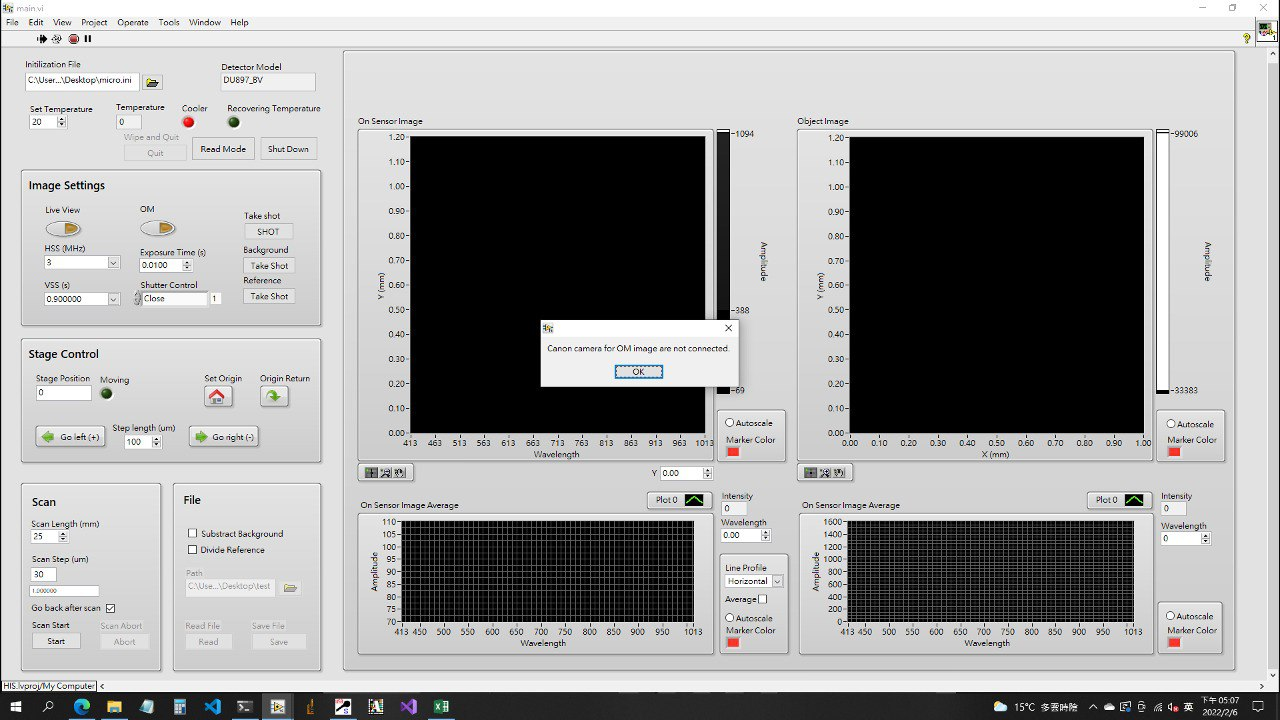
\includegraphics[width=\linewidth]{detectHW.jpeg}
    \caption{軟體會自行偵測硬體系統是否存在。}
    \label{figure: detect hardware}
\end{figure}
\subsubsection{TIFF存檔之擴充}
為了要使軟體在讀檔時能夠適當地調整UI,例如顯示實際的掃描尺寸,並且在掃描影像檔案內儲存影像分析與比較時必要的資訊,我將原本的實驗室IFD內的影像資料標籤進行了擴充,
表\ref{tab: new tag}列出這次所新增的所有標籤,這些標籤都在實驗室IFD區段,讀取方式與原本的標籤亦都相同。
要在存檔時新增標籤,可以如節\ref{section: saveTiff}所述一般以實驗室原有的Tiff存檔程式庫進行操作即可。
\begin{table}[ht]
    \begin{tabular}{lllll}
        ID & Type    & No. & Content               & Description             \\
        70 & 4(U32)  & 1   & HSI: Step Length      & in um                   \\
        71 & 11(SGL) & 1   & HSI: Real Y Dimension & in mm                   \\
        72 & 11(SGL) & 1   & HSI: Real X Dimention & in mm                   \\
        73 & 11(SGL) & 1   & HSI: VSS of iXon      & in sec                  \\
        74 & 4(U32)  & 1   & HSI: HSS of iXon      & in MHz                  \\
        75 & 1(U8)   & 1   & HSI: bkg exist?       & 1 for true, 0 for false \\
        76 & 1(U8)   & 1   & HSI: ref exist?       & 1 for true, 0 for false \\
        77 & 11(SGL) & 1   & HSI: Gain             &
    \end{tabular}
    \caption{新增的影像資料標籤。}
    \label{tab: new tag}
\end{table}

\subsubsection{背景/參考光譜之儲存}
至此,Tiff檔案已經存有多數必要的高光譜影像資訊,但使用者若進行反射率的觀測後,存檔時只會存下原始的觀測資料,背景/參考光譜影像
由於iXon每次擷取影像時的影像尺寸皆為固定,背景/參考光譜影像的尺寸與其所需的位元組數量,也可以由其他影像資料標籤,如影像長寬與data cube層數等標籤得知,因此在存檔
讀檔時軟體僅須由檔案最後,往回已推得的位元組開始讀取

\subsection{光譜量測與瀏覽實例}
本階段的軟體新功能開發,以高光譜影像資料的瀏覽與分析為主,我們加入了以下數個功能,來方便使用者對於系統掃描出的影像進行分析:
\begin{itemize}
    \item 在樣品影像上以滑鼠點選,或輸入數值,可以精確取讀取樣品的某位置的光譜。
    \item 在線光譜影像上以滑鼠點選,或輸入數值,可以讀取該影像垂直或水平的line profile。我們發現這樣的功能在衡量光源在空間中的均勻程度時相當有用。
    \item 在光譜顯示幕上,以滑鼠點選或輸入數值,可以在特定的波長處讀取光譜在該處的強度,在live view時這個功能也可以使用,因此也很適合用來確認是否準焦。
    \item 以上的瀏覽功能,在使用者進行點選或輸入時,相應的顯示幕上都會出現圖標標示出目前觀測的位置。
\end{itemize}
以下說明本系統以不同照明方式進行掃描時,在影像瀏覽介面所能進行的各項觀測操作,我們以同樣的橘色螢光片+銅網樣品,分別進行雷射光源照明的螢光光譜觀測,
以及高頻寬白光照明的反射光譜觀測,藉此印證系統的觀測能力與瀏覽功能。該螢光片樣品的結構,是在約$3.5mm^2$平方的橘色螢光片上,放上一個微小的銅網,銅網的正方形網格尺寸約為$127\mu m$。
\subsubsection{螢光光譜}
\begin{figure}
    \centering
    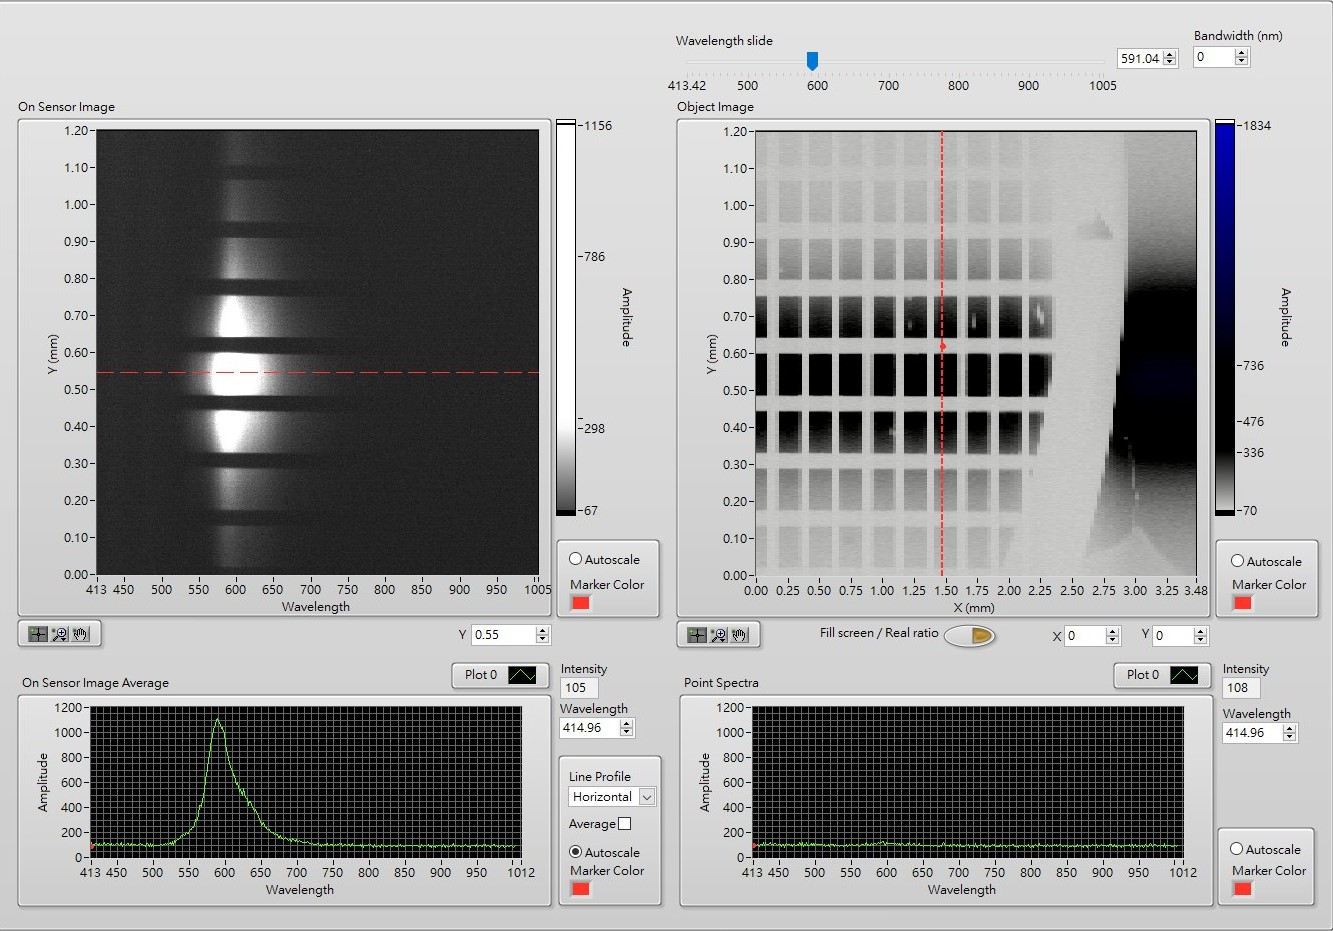
\includegraphics[width = 0.9\linewidth]{flourence.jpeg}
    \caption{雷射螢光光譜的觀測}
    \label{fig: flourence}
\end{figure}
所謂螢光觀測,是以405nm雷射平行光照明樣品,激發橘色螢光片僅在600nm左右才有的螢光,並在系統的成像鏡前將反射的405nm雷射光濾除,因此最終觀測到的影像,在網格下的螢光片
露出處,應觀測到集中於600nm左右的光譜,而在銅網格本身上,則因為銅網所反射的405nm雷射皆已被濾除,理應不會觀測到明顯的光譜特徵。

在圖\ref{fig: flourence}中,右側螢幕上所點擊到的位置,如螢幕上垂直紅色虛線上的紅點所示,該處為上層的銅網網格本身,右下方的光譜顯示幕上呈現的是紅點處的光譜,確實不會看見集中於600nm的光譜。
至於該螢幕上的紅色虛線處,與其上的紅點相同,都是隨著滑鼠點擊的位置移動,紅點是點擊位置,虛線則是紅點所在的掃描線,而該掃描線上的線掃描影像,則呈現在左側螢幕上。左側螢幕上,
亦有一條紅色虛線,也是隨著滑鼠在左側螢幕的點擊位置移動,虛線上的每一個像素,就是對應到左下方光譜螢幕的橫軸座標,而左下方光譜螢幕的縱軸,就是每個像素的強度,換句話說,該光譜螢幕即是
呈現出左側大螢幕上y=0.55處的光譜,也就是右側紅色虛線上y=0.55處的光譜。該處所在之處是露出的下層螢光片,因此左下光譜螢幕所呈現出的是一個集中在600nm處的光譜。

在左側的大螢幕上,也可以看見,所有亮帶都集中在600nm附近,與螢光片受雷射激發後的螢光波長一致。

由於本系統所儲存的影像資料符合正規的TIFF格式,訪間所有能夠讀取多層TIFF格式的影像瀏覽器,接能夠讀取本系統所擷取的影像。我們以免費、開源且普遍的ImageJ軟體,開啟一張同樣以雷射照明觀測本螢光片+銅網樣品的影像,
輕易的就可以對該影像進行各項處哩,包括沿波長軸的影像平均、影像比例的校正,並將多層的影像轉存為更易於在不同軟體、裝置或書面進行呈現的單張JPEG檔。
如圖\ref{fig: flourenceAvg}、\ref{fig: flourence628}、\ref{fig: flourence526}
所示,展現出本系統掃描檔案的使用彈性與廣泛的相容性。

\begin{figure}
    \centering
    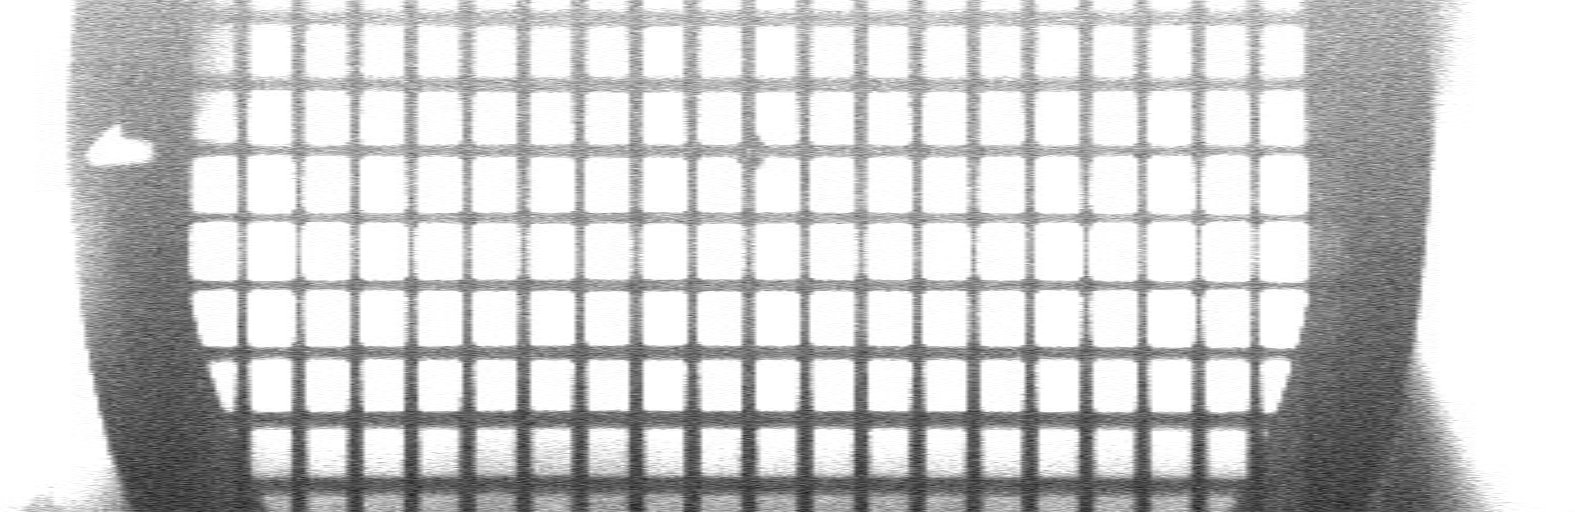
\includegraphics[width = 0.9\linewidth]{1211_10um_15msLaser-1.jpg}
    \caption{平均過後的螢光高光譜影像,以 405nm 雷射激發。本照片的比例經過調整,以符合樣品實物。實際大小約
    為 1.2×3.5mm,由 350 張單線光譜影像所接合而成}
    \label{fig: flourenceAvg}
\end{figure}

\begin{figure}
    \centering
    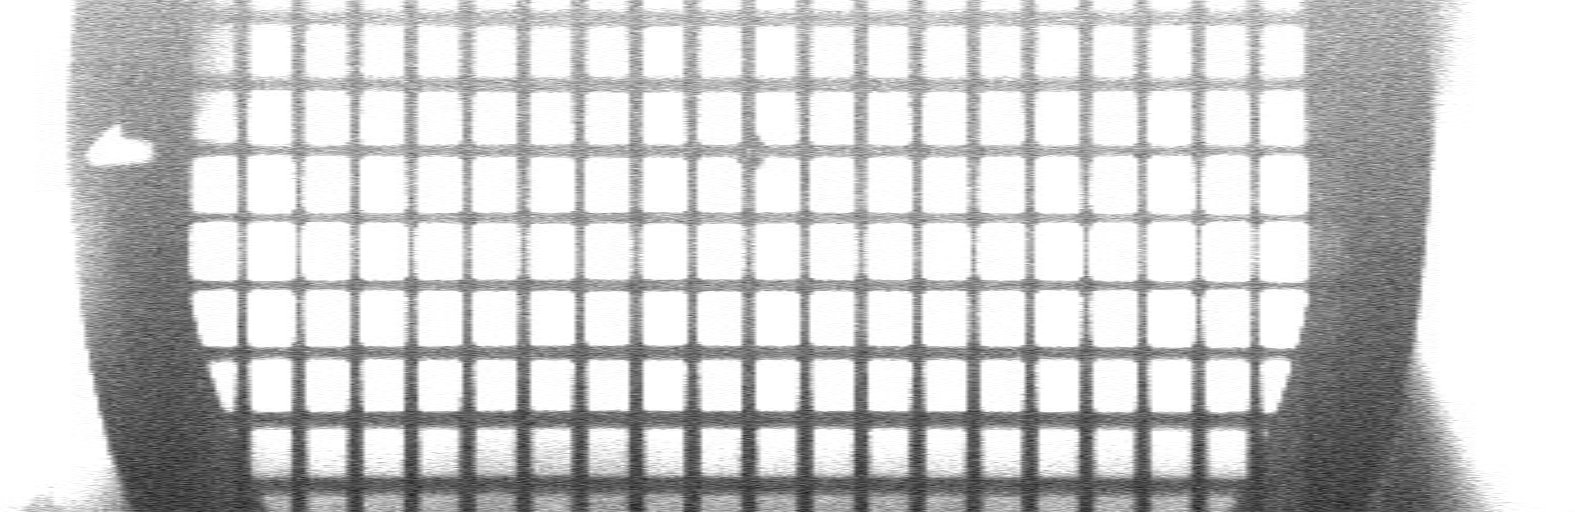
\includegraphics[width = 0.9\linewidth]{1211_10um_15msLaser-1.jpg}
    \caption{螢 光 的 高 光 譜 影 像, 僅 擷 取 約 在
    628nm 下的樣品影像。}
    \label{fig: flourence628}
\end{figure}

\begin{figure}
    \centering
    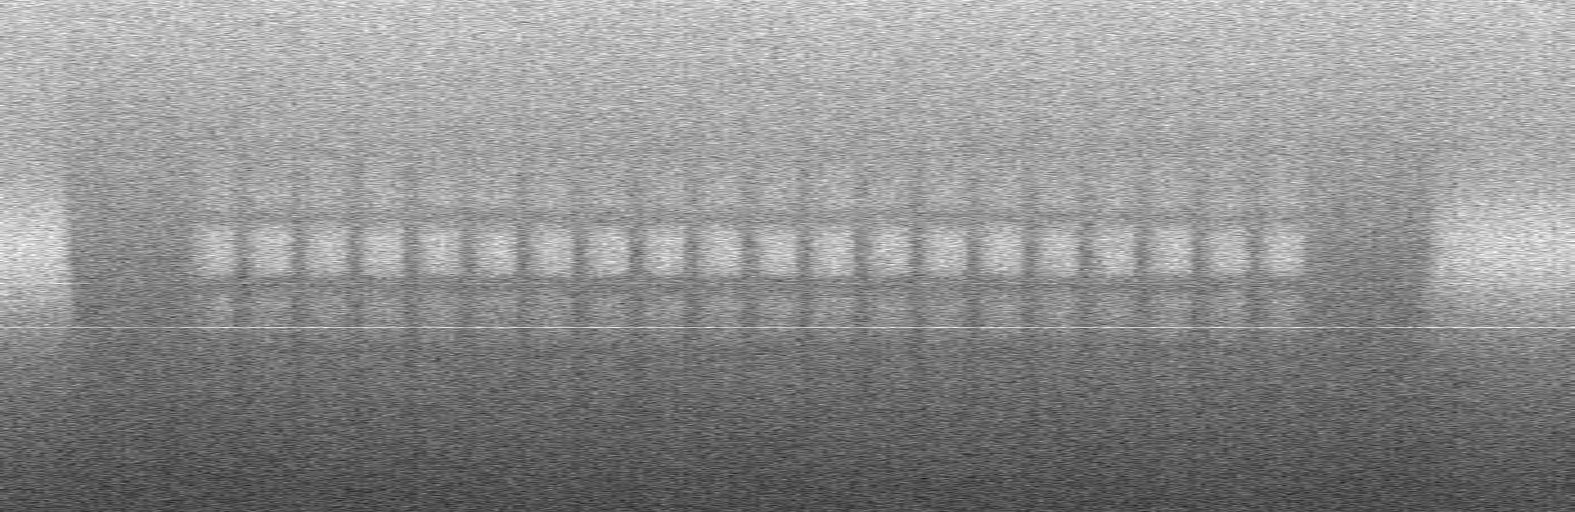
\includegraphics[width = 0.9\linewidth]{1211_10um_15msLaser.tiff137-1.jpg}
    \caption{螢光的高光譜影像,僅擷取約在 526nm 下
    的樣品影像,已經幾乎不可見。}
    \label{fig: flourence526}
\end{figure}

\subsubsection{反射光譜}
\begin{figure}
    \centering
    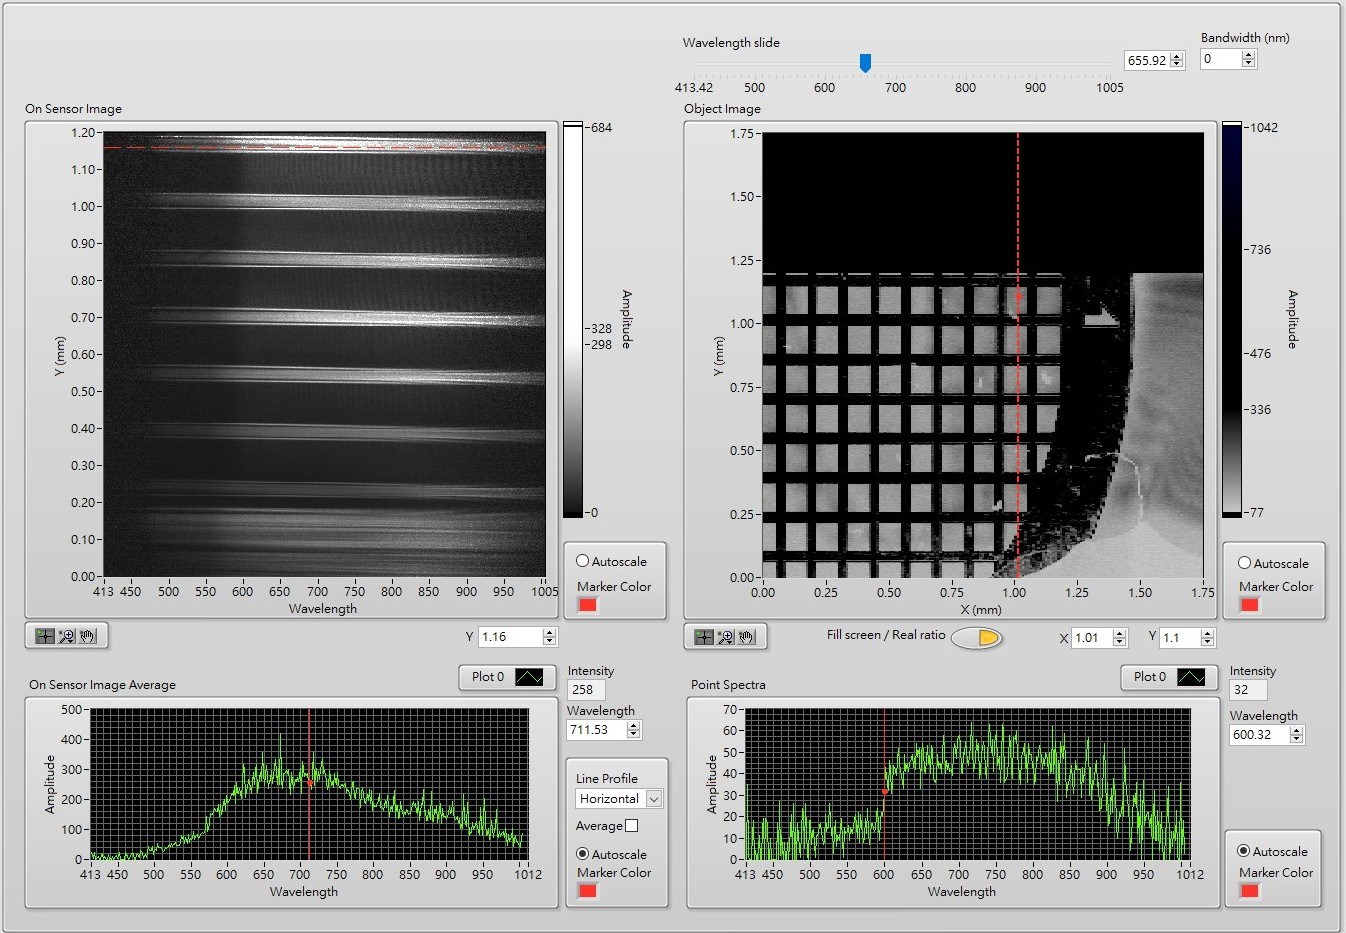
\includegraphics[width = 0.9\linewidth]{reflection (2).jpeg}
    \caption{反射光譜的觀測}
    \label{fig: reflec}
\end{figure}
同樣的螢光片+銅網樣品,在高頻寬的白光照射下,銅網網格處應會完整反射光源的光譜,而螢光片露出處則會較集中反射在600nm處。不過由於白光照明的強度極強,原始的反射光譜較難判別出其差異,
但本系統具有背景光譜與參考光譜的校準功能,能夠計算出樣品在每個位置與波長的反射率,更精確呈現出樣品的反射特徵。

圖\ref{figure: reflection}中,右下方的光譜螢幕呈現出右側大螢幕上紅點位置的反射率,由於觀測位置(紅點)在螢光片露出處,可以看見其反射率在600nm處有明顯的cutoff,橘色螢光片在橘色波長處有較強的反射率,顯然是合理的觀測結果。
而左側大螢幕上的紅色虛線則在y=1.16處,是銅網本身所在之處,因此左下方的螢幕呈現出銅網的反射光譜,就不會呈現出明顯的特徵。值得說明的是,本處右側螢幕上有開啟real ratio顯示模式,因此螢幕上的樣品影像已被調整為正確的實物比例,
與圖\ref{fig: flourence}中影像強制填滿正方形螢幕有所不同。

若反射光譜未經過背景光譜與參考光譜的校準,由於照明光源相當亮,其在整個可觀測的光譜範圍,都會有明顯的訊號。圖\ref{fig: reflec628}、\ref{fig: reflec526}同樣是以ImageJ調整並擷取的圖片,清楚呈現出觀測的原始影像(未經反射/背景光譜校準),在不同波長(無論大於或小於600nm)
都有相當強的訊號,與螢光光譜僅集中在600nm處,或是反射光譜經背景/參考光譜校準後,在600nm有cutoff的特徵,都相當不同。

透過圖\ref{figure: reflection}右側大螢幕的影像與圖\ref{fig: reflec628}、\ref{fig: reflec526}的比較,也可以發現經過參考光譜的校正後,不但反射率光譜不再存有照明光源的光譜特徵,
照明在空間上的上下不均勻也改善許多。本系統的最終目標是用於背焦面影像的觀測,而背焦面影像的取得勢必得透過反射照明的方式,其亦是一種反射光譜的觀測,因此此處所呈現的反射光譜瀏覽能力對於背焦面影像的觀測相當重要。

\begin{figure}
    \centering
    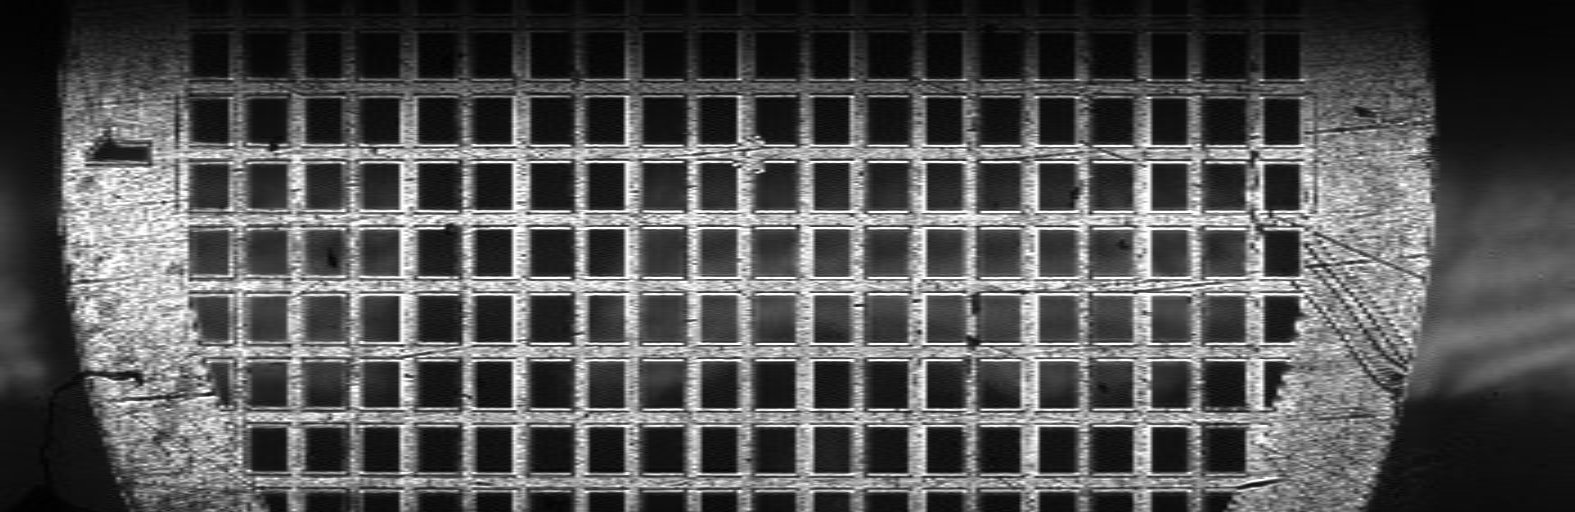
\includegraphics[width = 0.9\linewidth]{1211_10um_10ms-1.jpg}
    \caption{白 光 的 高 光 譜 影 像, 僅 擷 取 約 在
    628nm 下的樣品影像。}
    \label{fig: reflec628}
\end{figure}

\begin{figure}
    \centering
    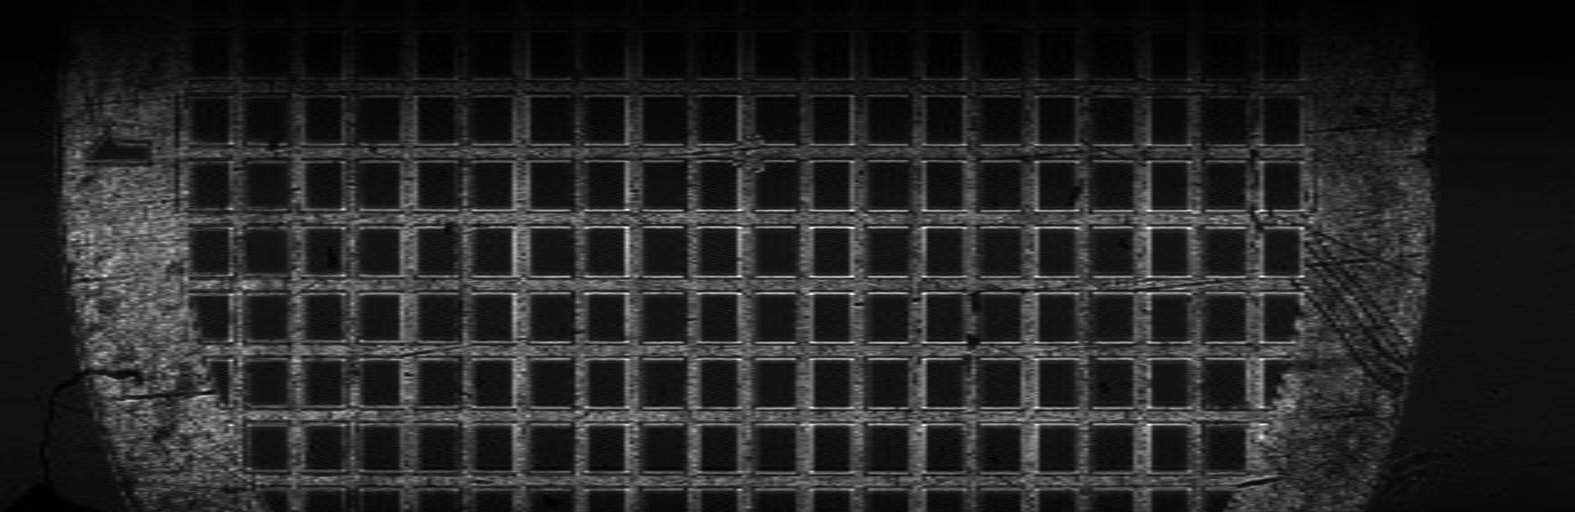
\includegraphics[width = 0.9\linewidth]{1211_10um_10ms137-1.jpg}
    \caption{白 光 的 高 光 譜 影 像, 僅 擷 取 約 在
    526nm 下的樣品影像,仍然相當清楚。}
    \label{fig: reflec526}
\end{figure}

\subsubsection{OBF Revisited}
\subsection{背焦面影像的探討}
\begin{figure}
    \centering
    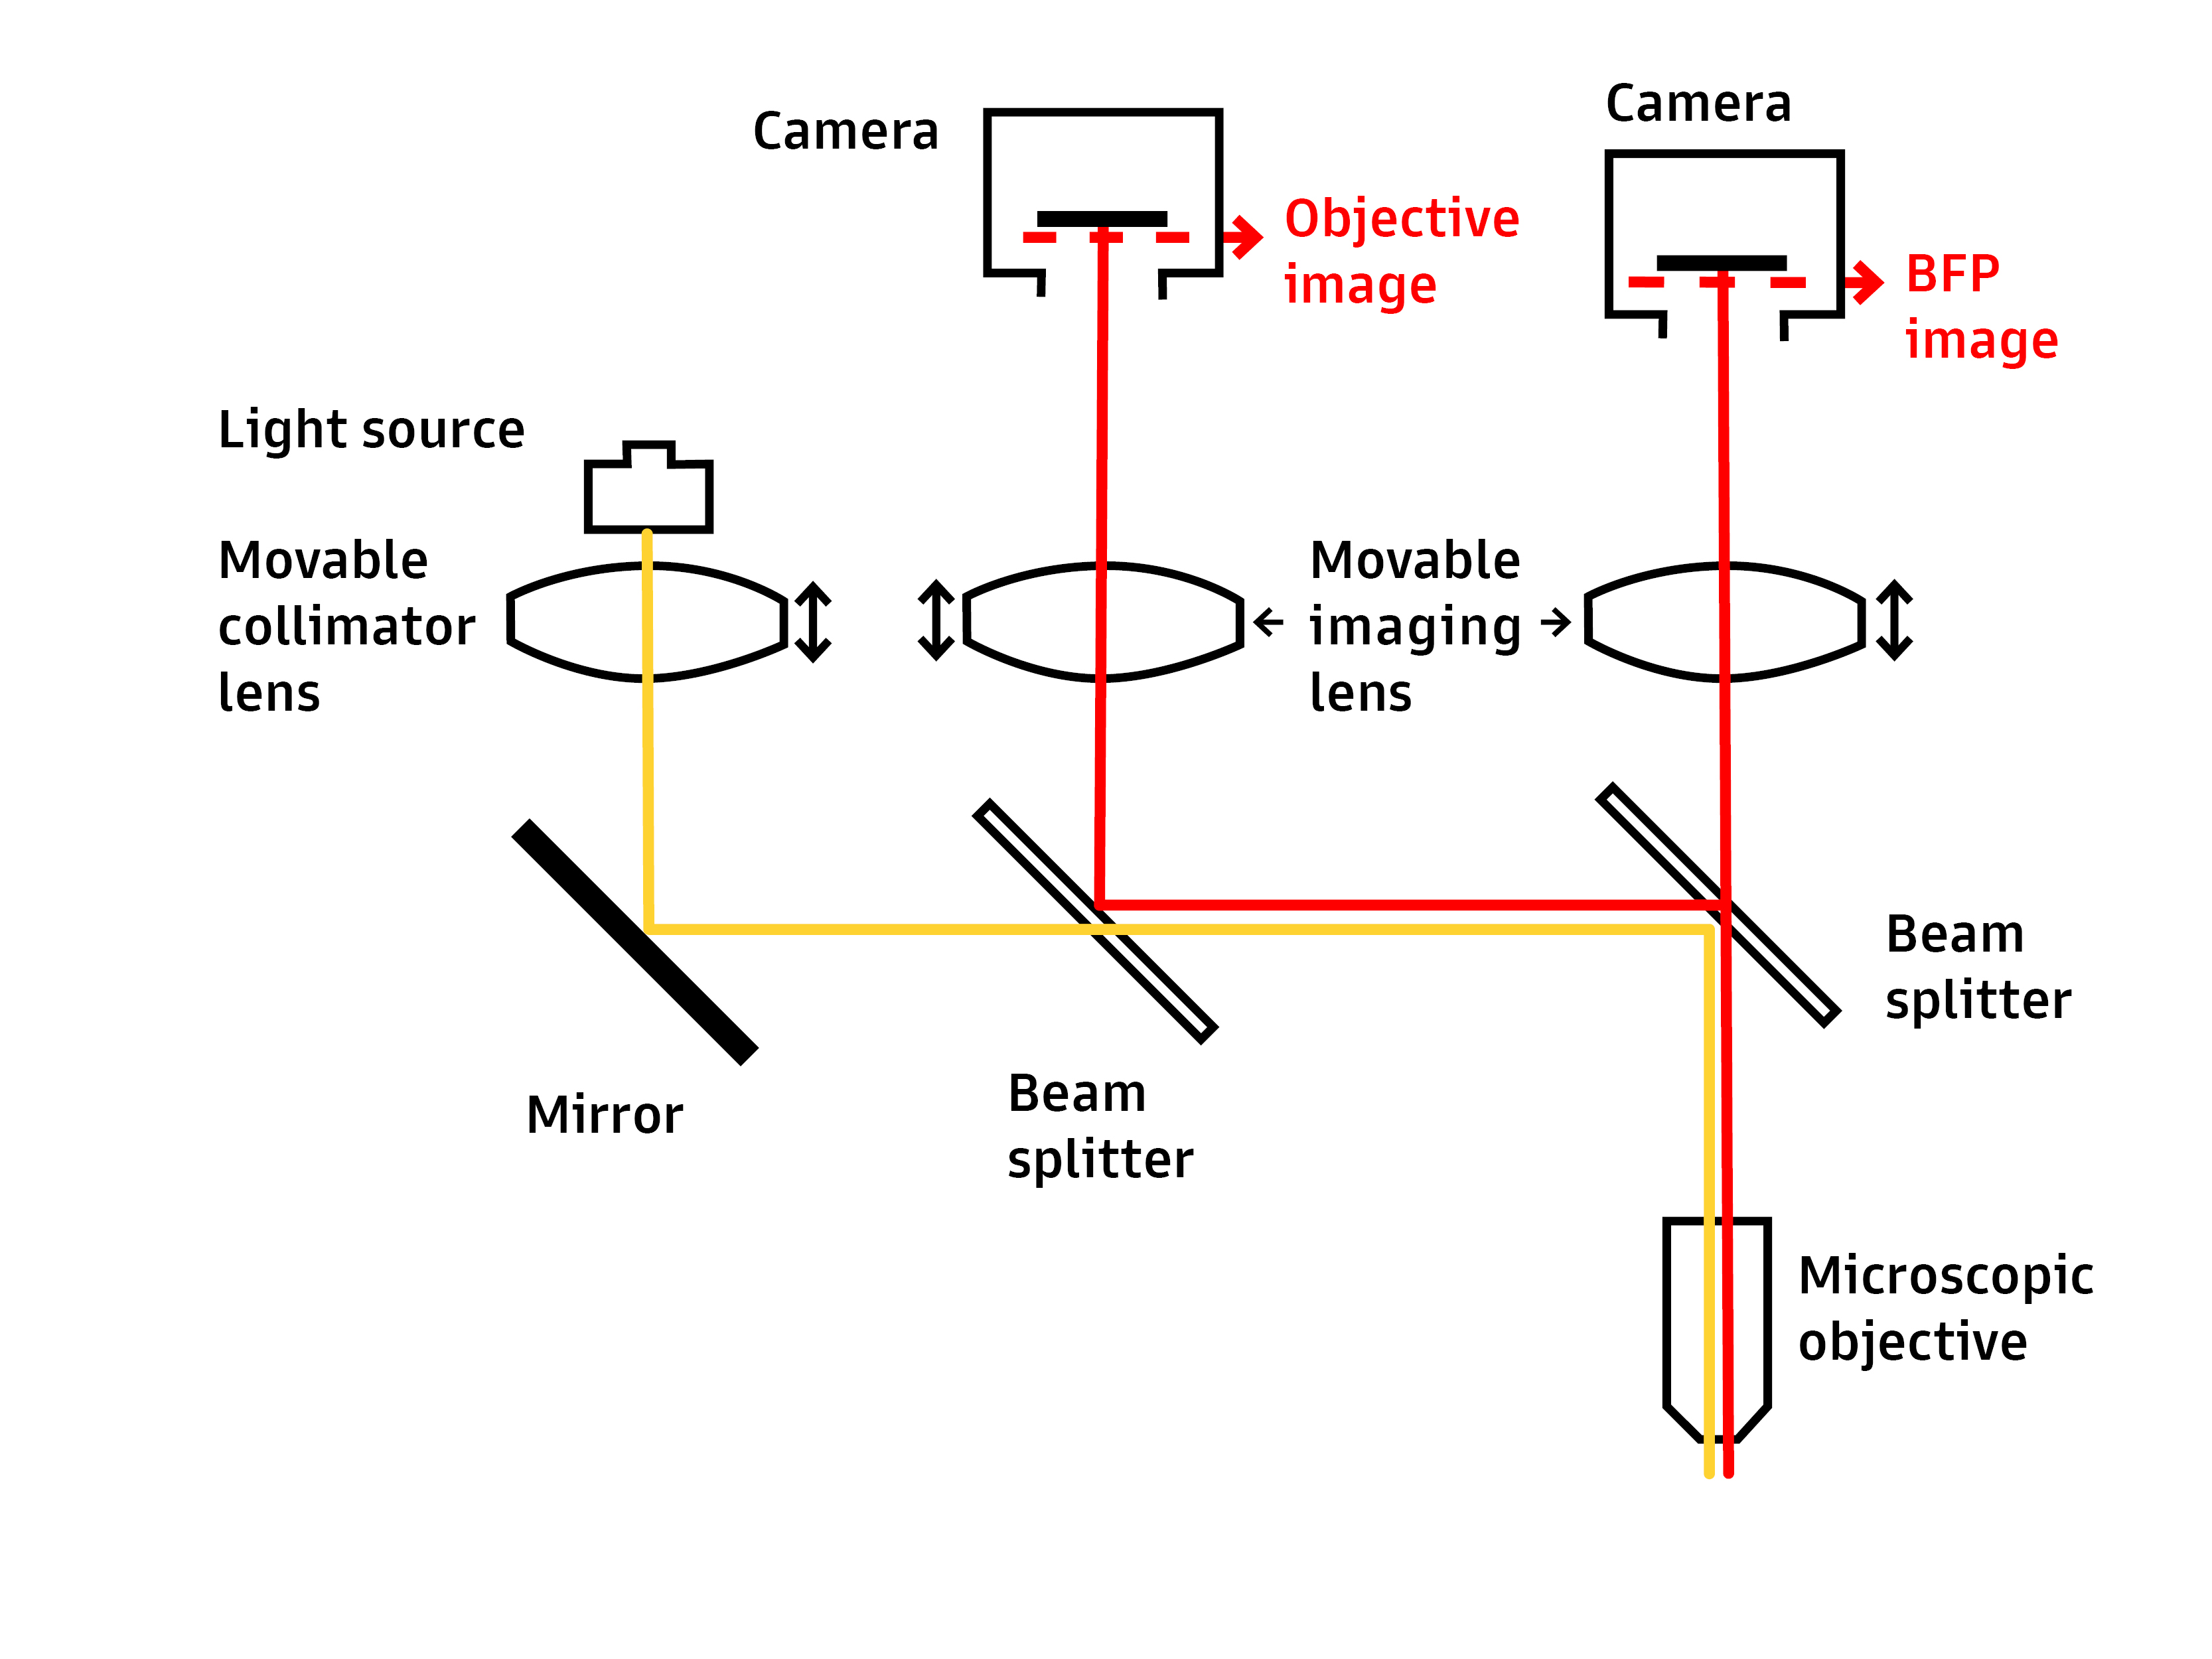
\includegraphics[width = 0.9\linewidth]{lightPath3.jpg}
    \caption{背焦面影像系統光路圖}
    \label{fig: bfp path}
\end{figure}
本系統奠基在平行光照明、掃描迅速,且具有完整反射光譜觀測功能等特性上,非常適宜結合背焦面影像的觀測技術,作為新穎材料表面特性的量測工具。
至此,本系統已具備高光譜掃描所必需的硬體架構與軟體功能,原則上僅需將原系統線光譜儀入射狹縫上的顯微影像,改換為樣品的背焦面影像,即具備背焦面影像的高光譜量測能力。
不過這樣的光學系統置換,實際上仍要面對許多問題,本研究中用於背焦面影像的光學系統,如圖\ref{fig: bfp path}所示,其與原先在節\ref{momentum}中設想者,有以下不同之處:
首先,由於原本的雙光源雙成像顯微影像系統,已將光學載板的空間大致用盡,我們希望能在不影響原系統的情形下先對背焦面影像的成像進行研究,因此未將原系統進行升級,
而是另組一部具有基礎觀測能力的顯微影像系統來使用。另外,原先設想背焦面影像系統能在背焦面影像與實域影像的觀測之間進行切換,但在系統開發的過程中,
我們發現在系統上以另一部相機同時觀測實域影像,以方便使用者對找尋欲觀測的樣品特徵,比背焦面/實域影像的切換功能較為實用,因此背焦面影像的觀測系統,
採用了與顯微影像觀測系統類似的雙成像架構,在圖\ref{fig: bfp path}中可以看到,兩部相機搭配不同焦距的成像鏡與成像位置,
經過數次調整後,可以同時分別觀察實域影像與背焦面影像。

為了方便對成像鏡與成像位置進行調整,我們以一部小巧的彩色CCD相機取代龐雜的線光譜儀+iXon影像系統,透過彩色CCD在可見光範圍附近的基礎光譜解析能力,
先對背焦面影像進行初步的研究。圖\ref{fig: 300 bfp}呈現出300 grating在LED白光照明、40倍顯微物鏡下,於本系統所觀測到的背焦面影像,同時在系統上的另一部相機,
則可以觀測到如圖\ref{fig: 300 real}的grating實域影像。關於grating的背焦面影像,則能以圖\ref{fig: 500 bfp}來相互瞭解比較。
grating在白光照射下,會將同樣波長的光線以同樣的角度反射;而背焦面影像的主要性質,則是會將物鏡前同樣角度的入射光線,成像於同樣的位置(見節\ref{bfpimage}),
因此,在grating的背焦面影像上,同樣波長的光線應會被成像於背焦面影像影像的同樣位置。圖\ref{fig: 500 bfp}與\ref{fig: 300 bfp}中皆可看見不同顏色(不同波長)的
光線被成像在不同位置,而產生類似彩虹一般的顏色分布。透過兩圖之間的比較,也可以看見,由於不同波長的光線經500 grating反射後散開的角度會比300 grating來的更開,
因此圖\ref{fig: 500 bfp}上不同顏色的位置分布區隔更明顯。另外,500 grating的各階干涉之間的距離也理應會比300 grating來的更遙遠,也可以透過兩圖的比較來驗證,
圖\ref{fig: 300 bfp}中300 grating的各階干涉非常接近,導致有明顯的重疊。

\begin{figure}[h]
    \centering
    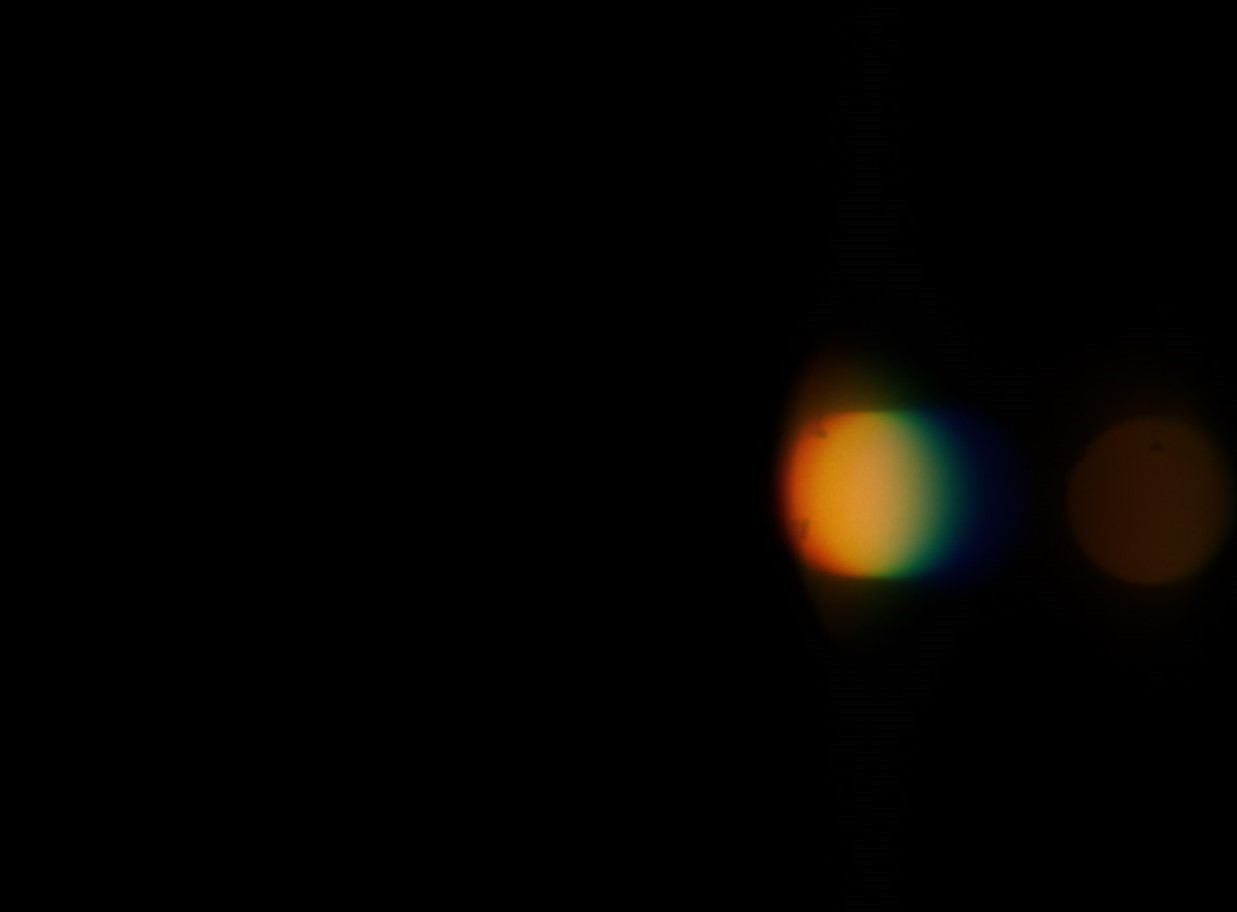
\includegraphics[width = 0.8\linewidth]{300bfp.jpeg}
    \caption{BFP of 300 grating}
    \label{fig: 300 bfp}
\end{figure}

\begin{figure}[h]
    \centering
    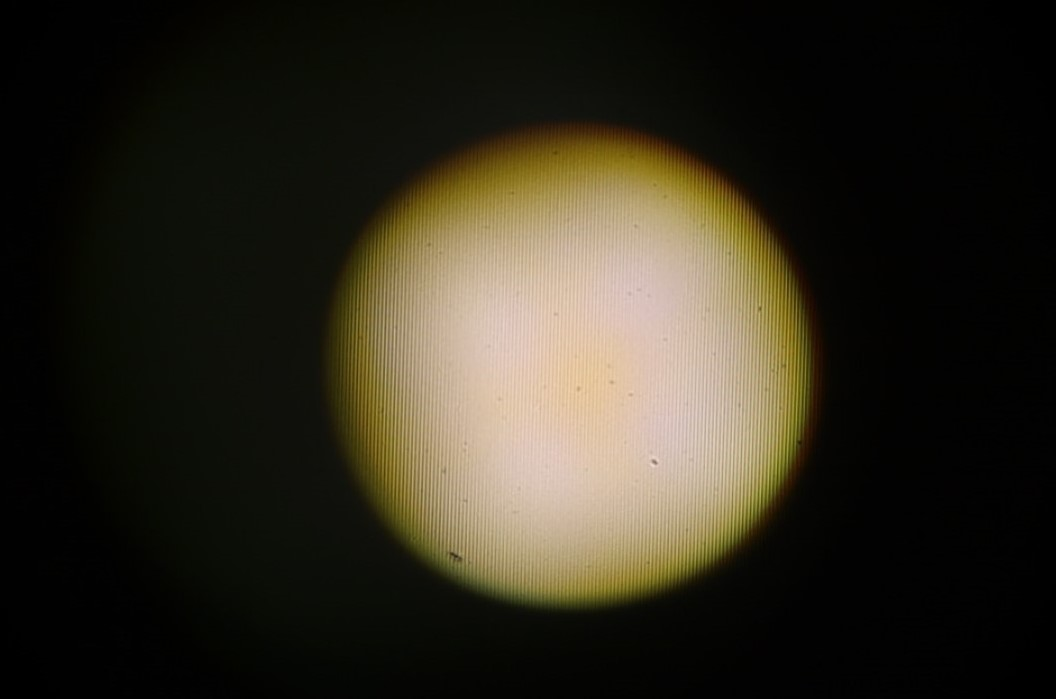
\includegraphics[width = 0.8\linewidth]{300real.jpeg}
    \caption{Real space image of 300 grating}
    \label{fig: 300 real}
\end{figure}

\begin{figure}[h]
    \centering
    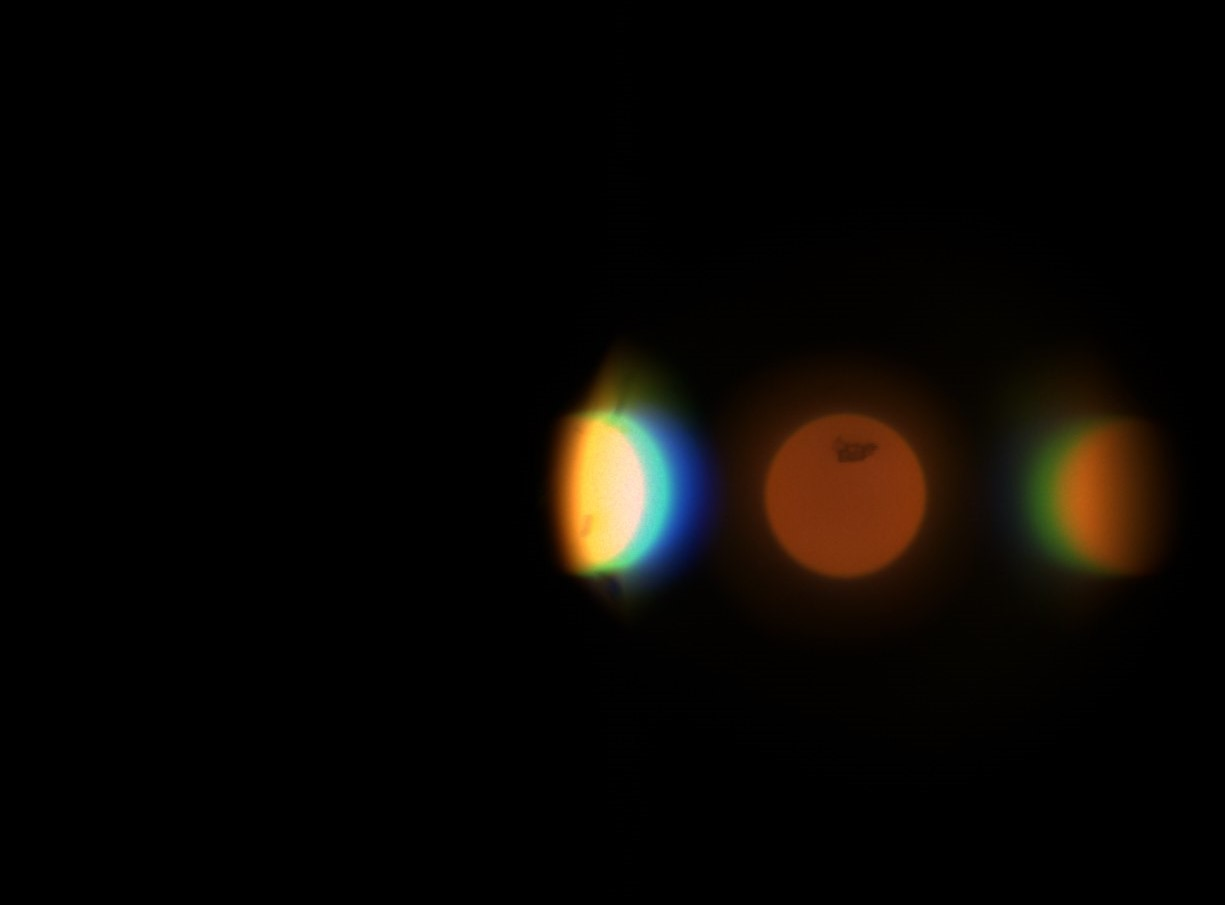
\includegraphics[width = 0.8\linewidth]{500bfp.jpeg}
    \caption{BFP of 500 grating}
    \label{fig: 500 bfp}
\end{figure}

透過上述的初步研究,已印證該光學系統具有基礎的背焦面影像觀測能力,若能將彩色CCD換回線光譜儀+iXon的影像系統,即能實線背焦面影像的高光譜影像量測,
不過由於影像系統的轉移勢必牽涉大量參數的重新校正,且背焦面影像的線掃描尚有其他問題須待解決,礙於研究時間的限制,背焦面高光譜影像系統的整合須待由後續的研究者繼續開發,
下章則會簡述該技術尚需克服的挑戰。

\section{未來展望}
在本研究中我們已經成功地建立起一部以線掃描技術為基礎,具有顯微高光譜影像觀測能力的量測系統。系統可以適用雷射螢光的光譜量測,同時,由於採用平行光照明的關係,也非常適合反射光譜的量測,
並能針對影像感測器的背景(雜訊)光譜,或是光源的參考光譜進行校準,以反射率來呈現樣品的反射光譜。此外,我們也對背焦面影像系統進行了初步的開發,並印證其觀測背焦面影像的能力。
再結合本系統軟體上豐富的光譜瀏覽功能,以及儲存為TIFF檔後與其他影像處理軟體的高度相容性,我們認為本系統已具備相當完整的高光譜影像觀測功能性。且由於系統參數皆以便攜且易於修改的.init檔方式
儲存,要將線掃描影像系統再與背焦面影像系統進行結合,應具有相當高的可行性,不過由於研究時間的限制,該部分的系統整合需留待後續研究者繼續開發,

以本研究的開發經驗來看,我們認為,背焦面影像系統與線掃描顯微系統的整合,尚有以下的挑戰需克服,是未來研究者值得探討的方向:
\begin{enumerate}
    \item 當我們對樣品進行線掃描時,是透過移動樣品來改變掃描線的位置,所以所有的影像系統皆是固定不動的。但當我們要對樣品的背焦面影像進行掃描時,便無法以這樣的方式掃描,因為
    無論如何移動樣品,背焦面影像的成像位置都是固定的。要如何在線掃描儀的入射狹縫處「移動背焦面影像」,將是一個關鍵的課題。若同樣要維持線掃描儀與影像感測器不動的設定,
    則可能要移動包括顯微物鏡與成像鏡在內的整個背焦面影像系統。
    \item 在顯微實域影像觀測時,就算在線掃描影像下,也能大致透過入射狹縫上單軸的空間特徵,確認成像是否清楚並準確對焦。然而,當入射狹縫上的影像為背焦面影像時,
    由於背焦面影像已不再有樣品的空間特徵,我們很難以背焦面影像的來確認對焦狀態。這也是我們在最後的背焦面影像系統中採用平行雙成像架構的原因之一,觀測時可以先以時域影像調整對焦,
    並同時觀測背焦面影像是否清楚。但要如何確認時域影像清楚時,背焦面影像也是準焦的? 這牽涉到兩個光路之間的匹配與校正,亦是值得深究的方向。
\end{enumerate}

除此之外,我們已經完整建立起的顯微線掃描高光譜影像系統,能夠快速地建立大範圍的顯微高光譜影像,單軸的線掃描方式使速度提升,操作也更簡單。採用平行光照明的架構,使系統除了螢光以外,
也很適合做反射光譜的量測。再加上完整的光譜瀏覽功能,對於新穎材料的表面量測、產品的微結構驗證等,都可以提供極有效率的觀測功能。不過針對本系統目前的狀態,我們仍然認為掃描速度有提升
的空間。線掃描技術的初衷是提升掃描的速度,然而線光譜儀需搭配二維影像感測器使用,與傳統光譜儀搭配的一維影像感測器相比,其讀取速度確實較慢。我們所使用的iXon感測器,
最後也導致系統的掃描速度不如預期。若換用不同的二維影像感測器進行觀測,是否能在近一步提升其掃描速度,也相當值得深究。

\printbibliography
\end{document}